\documentclass{article}

\usepackage[utf8]{inputenc} % allow utf-8 input
\usepackage[T1]{fontenc}    % use 8-bit T1 fonts
\usepackage{hyperref}       % hyperlinks
\usepackage{url}            % simple URL typesetting
\usepackage{booktabs}       % professional-quality tables
\usepackage{amsfonts}       % blackboard math symbols
\usepackage{nicefrac}       % compact symbols for 1/2, etc.
\usepackage{microtype}      % microtypography
\usepackage{siunitx}
\usepackage{lipsum}
\usepackage{fancyhdr}       % header
\usepackage{graphicx}       % graphics
\usepackage{float}          % For more control over figure 
\graphicspath{{media/}}     % organize your images and other figures under media/ folder
\usepackage{amsmath}
\usepackage{amssymb}
\usepackage{amsfonts}
\usepackage{listings}
\usepackage{titlesec}
\usepackage{needspace}
\usepackage{glossaries}
\usepackage{enumitem}
 % imports packages 
\usepackage{color}
\usepackage{listings}

\definecolor{GrayCodeBlock}{RGB}{241,241,241}
\definecolor{BlackText}{RGB}{110,107,94}
\definecolor{RedTypename}{RGB}{182,86,17}
\definecolor{GreenString}{RGB}{96,172,57}
\definecolor{PurpleKeyword}{RGB}{184,84,212}
\definecolor{GrayComment}{RGB}{170,170,170}
\definecolor{GoldDocumentation}{RGB}{180,165,45}

\lstdefinelanguage{Rust}
{
    columns=fullflexible,
    keepspaces=true,
    frame=single,
    framesep=0pt,
    framerule=0pt,
    framexleftmargin=4pt,
    framexrightmargin=4pt,
    framextopmargin=5pt,
    framexbottommargin=3pt,
    xleftmargin=4pt,
    xrightmargin=4pt,
    backgroundcolor=\color{GrayCodeBlock},
    basicstyle=\ttfamily\color{BlackText},
    keywords={
        true,false,
        unsafe,async,await,move,
        use,pub,crate,super,self,mod,
        struct,enum,fn,const,static,let,mut,ref,type,impl,dyn,trait,where,as,
        break,continue,if,else,while,for,loop,match,return,yield,in
    },
    keywordstyle=\color{PurpleKeyword},
    ndkeywords={
        bool,u8,u16,u32,u64,u128,i8,i16,i32,i64,i128,char,str,
        Self,Option,Some,None,Result,Ok,Err,String,Box,Vec,Rc,Arc,Cell,RefCell,HashMap,BTreeMap,
        macro_rules
    },
    ndkeywordstyle=\color{RedTypename},
    comment=[l][\color{GrayComment}\slshape]{//},
    morecomment=[s][\color{GrayComment}\slshape]{/*}{*/},
    morecomment=[l][\color{GoldDocumentation}\slshape]{///},
    morecomment=[s][\color{GoldDocumentation}\slshape]{/*!}{*/},
    morecomment=[l][\color{GoldDocumentation}\slshape]{//!},
    morecomment=[s][\color{RedTypename}]{\#![}{]},
    morecomment=[s][\color{RedTypename}]{\#[}{]},
    stringstyle=\color{GreenString},
    string=[b]"
}

 % imports code formatting 

%Header
\pagestyle{fancy}
\thispagestyle{empty}
\rhead{ \textit{ }} 

% Update your Headers here
\fancyhead[LO]{DeepCausality: A Hypergeometric Framework for Context-Aware Causal Reasoning in Rust}
  
%% Title
\title{DeepCausality: A Hypergeometric Framework for Context-Aware Causal Reasoning in Rust}

%% Author
\author{
  Marvin Hansen \\
  \texttt{marvin.hansen@gmail.com} \\
  Draft: \today
}


\begin{document}
\maketitle

%% Abstract
\begin{abstract}

The rapid advancement of artificial intelligence, particularly Large Language Models (LLMs), has unlocked powerful capabilities in pattern recognition and information synthesis. However, these systems often exhibit fundamental limitations in genuine explainability, struggle with dynamic real-time contextual relevance, and operate primarily on correlational understanding rather than explicit causal mechanisms, leading to issues like "hallucinations" and unreliability with out-of-distribution data or tasks requiring deep, verifiable understanding. This paper introduces DeepCausality, an open-source computational causality framework implemented in Rust, designed to address these limitations by enabling the construction and reasoning over explicit, context-aware causal models.


DeepCausality offers a robust system where causal models are deeply embedded within rich, multidimensional, and dynamic contexts. Unique to the framework is its hypergraph-based representation of both causality (via CausaloidGraphs of recursively composable, operational Causaloids – testable causal functions) and context (via hypergraphs of Contextoids representing data, time, space, and spacetime, supporting both Euclidean and non-Euclidean relational information). This structural approach facilitates transparent composability, the creation of static and dynamic causal models, deterministic evaluation with pathways for probabilistic extension, and complex interactions with multiple shared or distinct contexts. A key feature is the Causal State Machine (CSM), enabling the direct linkage of causal inferences to deterministic actions for building dynamic control and supervision systems.


The paper details DeepCausality’s architecture, its theoretical foundations rooted in operational causality and a layered reasoning model, and its Rust implementation which leverages the language's type system for safety, performance, and expressiveness. We discuss current limitations, compare DeepCausality with established causal paradigms, and argue for its significance as a foundational causal engine. Furthermore, we outline a future vision for Grounded Intelligent Agency, proposing a synergistic fusion of DeepCausality with LLMs, where LLMs act as perception and hypothesis generation layers and DeepCausality provides the rigorous analytical and verification core for mechanistic understanding and explainable action. DeepCausality is available online is and hosted at the Linux Foundation.

\begin{center}
    \url{https://deepcausality.com}
\end{center}

\end{abstract}


%% keywords
\keywords{Computational Causality \and Context-Aware Reasoning \and Causaloid \and Quantum Gravity \and  Causal Models \and Explainable AI \and Hypergeometric Models \and Causal State Machines \and Grounded Intelligent Agency}

\newpage

%% Table of Contents 
\tableofcontents

%% Content

%% Section 1: Intro (Problem)
\section{Introduction}
\label{sec:introduction}

The rapid ascendancy of Artificial Intelligence (AI), spearheaded by transformative technologies like Large Language Models (LLMs), has unveiled unprecedented capabilities in processing information and mimicking human-like responses. Yet, this progress casts a stark light on persistent, fundamental limitations: many contemporary AI systems, despite their sophistication, often operate as "black boxes," struggle to genuinely comprehend or adapt to dynamic real-world contexts, and are predominantly rooted in correlational pattern-matching rather than explicit causal mechanisms. 
This foundational gap frequently leads to unreliability, "hallucinations," and a lack of verifiable understanding, critically undermining trust and hindering their application in domains demanding high stakes, robustness, and true explainability. The development of AI that can not only predict but also \textit{explain} and \textit{reliably act} based on a deep understanding of cause and effect remains a paramount scientific and engineering endeavor.

This paper introduces DeepCausality, a paradigm shift towards computational causality, engineered from first principles in Rust. DeepCausality is an open-source framework, hosted at the Linux Foundation and accessible at \url{https://deepcausality.com}, designed to enable the construction, execution, and rigorous management of explicit, context-aware, and explainable causal models. It moves beyond mere statistical associations to model the generative mechanisms underlying observed phenomena, providing a pathway for AI systems to reason about cause and effect within intricate, multi-dimensional, and dynamically evolving environments. 
The framework's unique "hypergeometric" nature refers to its core reliance on hypergraph structures for representing both the rich tapestry of context and the complex web of causal relationships, offering a new level of expressiveness and analytical depth.

DeepCausality’s core contributions are architected to address the identified limitations of current AI and provide a robust foundation for causally-grounded intelligence:
\begin{itemize}
    \item \textbf{A Novel Hypergraph-based Context Engine:} At its heart, DeepCausality features a sophisticated engine for managing context. This moves beyond simple conditioning variables to enable the creation of intricate context hypergraphs populated by \textit{Contextoids} – specialized nodes representing rich, multi-dimensional information encompassing Data, Time, Space, and SpaceTime. This inherently supports dynamically adjustable contexts, the simultaneous integration of information from multiple distinct context hypergraphs (potentially with differing Euclidean or non-Euclidean geometries), and grounds causal reasoning in a highly nuanced and comprehensive understanding of the operational environment.
    \item \textbf{Structurally Composable Causal Modeling:} DeepCausality introduces \textit{Causaloids} – encapsulated, testable causal functions – as the fundamental building blocks of causal models. These are organized within \textit{CausaloidGraphs}, which are themselves hypergraphs explicitly representing intricate causal relationships. Crucially, this architecture employs recursive isomorphic causal data structures: nodes within a CausaloidGraph can themselves be entire sub-graphs or collections of other causes. This enables the intuitive, modular construction of deeply complex, layered causal systems where macro-level phenomena can be decomposed into interacting micro-level mechanisms, ensuring transparent composability.
    \item \textbf{The Causal State Machine (CSM) for Actionable Intelligence:} Bridging the gap between causal understanding and effective intervention, the CSM is architected to manage interactions between causal models and their contexts. Based on the collective causal inference derived—the identification of specific active causes or system states—the CSM deterministically initiates predefined actions, facilitating the creation of complex, dynamic control and supervision systems that respond with causally-reasoned precision.
    \item \textbf{Implementation in Rust for Performance and Reliability:} Recognizing the demanding requirements of a sophisticated causal reasoning engine operating on potentially vast and dynamic data, DeepCausality is implemented in Rust. This choice leverages Rust’s high-performance characteristics, memory safety guarantees, and expressive type system to build an efficient, robust, and reliable foundational causal engine.
    
\end{itemize}

The theoretical underpinnings of DeepCausality draw inspiration from operational views of causality and a philosophical re-evaluation of effect propagation, guiding its design towards flexibility and adaptability in modeling emergent causal structures. This paper details the complete architecture of DeepCausality, its conceptual foundations, and its Rust implementation. We analyze its current limitations, compare it with established causal paradigms, and articulate its significance as a foundational technology. Looking ahead, we elaborate on the future direction of architecting Grounded Intelligent Agency by envisioning a synergistic fusion of DeepCausality’s rigorous causal reasoning with the perceptual and generative capabilities of LLMs, aiming to create AI systems that are not only broadly aware but also deeply and verifiably understand the causal fabric of the world they operate in. We begin with the motivation for this work, followed by a review of related background, before delving into the core of the DeepCausality framework.

\newpage
%% Section 2: Motivation 
\section{Motivation}
\label{sec:motivation}

Recent advancements in artificial intelligence, particularly in deep learning (DL) and large language models (LLMs), have demonstrated remarkable proficiency in processing vast amounts of data, recognizing intricate patterns, and generating human-like text and responses \cite{lecun2015deep, schmidhuber2015deep, goodfellow2016Deep}. These systems can summarize information, answer complex questions, and even generate creative content, leading to their rapid adoption across numerous fields. However, alongside these successes, a closer examination reveals inherent limitations stemming from their primarily correlation-based foundations.

\subsection{Limitations of corelation based methods}
\label{subsec:limits}   

The impressive achievements of deep learning models are undeniable, having revolutionized fields from natural language processing to computer vision \cite{lecun2015deep, schmidhuber2015deep,goodfellow2016Deep, Scholkopf2021Toward}. However, these successes are largely predicated on their strength as statistical techniques capable of sophisticated pattern learning or ``curve fitting'' over vast datasets \cite{pearl2018theoretical, Scholkopf2021Toward}. This foundation gives rise to several inherent limitations, hindering their ability to achieve genuine understanding and robust, trustworthy reasoning, particularly in complex, dynamic, and high-stakes environments \cite{pearl2018theoretical, Scholkopf2021Toward, Kaddour2022Causal}. These limitations include significant challenges in generalizing beyond the training data space and handling distribution shifts \cite{Scholkopf2021Toward}, vulnerability to subtle input perturbations \cite{Scholkopf2021Toward}, a lack of transparency and interpretability which is critical in high-stakes applications \cite{Scholkopf2021Toward}, and a fundamental inability to inherently reason about interventions or causality \cite{pearl2018theoretical, Scholkopf2021Toward, Kaddour2022Causal}.

\textbf{Correlation does not imply Causation}: Deep learning models excel at identifying and exploiting statistical correlations within data \cite{Scholkopf2021Toward, Kaddour2022Causal, Bareinboim2012causal, Guo2018Survey}. However, as famously articulated by Judea Pearl \cite{Pearl2009Causality}, these achievements are largely based on sophisticated "curve fitting" or pattern interpolation over vast datasets\cite{Pearl2009Causality, Bareinboim2020On, Scholkopf2021Toward}. They do not inherently distinguish between correlation and causation \cite{Pearl2009Causality, Bareinboim2012causal, Scholkopf2021Toward, Kaddour2022Causal, wolff2018solutions, Peters2017Elements, Guo2018Survey, Guyon2010Causality}. Machine learning applied to observational data \cite{Peters2017Elements}, where predictive variables are not under the learner's control \cite{Bareinboim2012causal}, can typically only learn correlations \cite{Bareinboim2012causal, Peters2017Elements}. Consequently, a model might learn that factor A is highly correlated with outcome B \cite{Bareinboim2012causal}, but it cannot, without explicit causal information or intervention capabilities \cite{Pearl2009Causality, Bareinboim2012causal, Scholkopf2021Toward, Kaddour2022Causal, Peters2017Elements, Lattimore2016Causal, Lee2018Structural}, determine if A causes B, B causes A, or if a hidden common cause C influences both \cite{Bareinboim2012causal, Peters2017Elements}. This limitation is critical for decision-making \cite{Bareinboim2012causal, Kaddour2022Causal, Wang2020Causal, Lu2020Regret, Aglietti2020Causal}, as acting upon a spurious correlation \cite{Bareinboim2012causal, Peters2017Elements, Lu2020Regret} can lead to ineffective or even detrimental interventions \cite{Bareinboim2012causal, Lu2020Regret}.

\textbf{The Independent and Identically Distributed (IID) Data Assumption:} Many foundational machine learning algorithms, and by extension some deep learning approaches, assume that data points are drawn independently from the same underlying distribution \cite{jordan2015machine}. 
This assumption is frequently violated in real-world scenarios \cite{Scholkopf2021Toward, Kohavi2009Controlled}. Financial market data exhibits temporal dependencies and regime shifts \cite{ Pena2016Multivariate}; social network data is characterized by complex interdependencies \cite{baykal2022bandit, Wang2020Causal}; industrial sensor data may be autocorrelated \cite{binkowski2017autoregressive, Li2020Enhanced, Runge2019Detecting}. When the IID assumption breaks down, the performance and reliability of DL models can degrade significantly \cite{Scholkopf2021Toward}, as the patterns learned during training may no longer hold in production \cite{Scholkopf2021Toward}. DARPA itself has noted the limitations of treating "each data set as an independent, uncorrelated input" and the need to model "underlying causal mechanism[s]" \cite{DARPA_ANSR}.

\textbf{The "Black Box" Problem and Lack of Genuine Explainability}: Deep neural networks, especially those with billions or trillions of parameters like modern LLMs, are often described as "black boxes". \cite{Scholkopf2021Toward, Kaddour2022Causal}. While techniques from Explainable AI (XAI) can provide post-hoc rationalizations or highlight influential features, they often do not reveal the true internal computational path or the underlying reasoning process in a verifiable way \cite{Scholkopf2021Toward, Kaddour2022Causal, wolff2018solutions}. Deep learning models learn statistical patterns and associations, but may not capture underlying causal mechanisms \cite{Scholkopf2021Toward}. The opacity makes it difficult to debug models \cite{Moraffah2020Causal}, and is a potential liability when using deep learning for problem domains medical diagnosis, where human users might like to understand how a system made a decision \cite{Moraffah2020Causal}. Such opacity can also lead to issues of bias \cite{Moraffah2020Causal}. Model explanations allow us to argue for model decisions and exhibit the situation when algorithmic decisions might be biased or discriminating, and precise explanations may facilitate model debugging and error analysis \cite{Moraffah2020Causal}. It is important to build trust, particularly in critical applications \cite{Moraffah2020Causal}.

\textbf{Knowledge Cut-off and Real-Time Relevance: }LLMs are trained on data up to a specific point in time. Consequently, they lack knowledge of events, discoveries, or shifts in the world that occur after their training data concluded. While "search grounding" – augmenting LLMs with real-time internet search – provides access to current facts, it does not inherently equip the model with an understanding of evolving dynamics or the ability to integrate new information into a coherent, evolving causal model of a system's state \cite{Scholkopf2021Toward}. The interpretation of new information is still performed through the lens of patterns learned from historical data \cite{Scholkopf2021Toward}.


\textbf{Lack of Innate Conceptualization of Time, Space, and Causality: } While deep learning models can learn patterns related to these concepts from data, they do not possess them as foundational, structured elements of their reasoning framework in the way humans do \cite{Davis2015Commonsense, Marcus2018Deep, Pearl2009Causality, Scholkopf2021Toward}. Rather, true AI requires an innate grasp of fundamental concepts like time, space, and causality \cite{Pearl2009Causality, Scholkopf2021Toward, Kaddour2022Causal, bishop2020artificialintelligencestupidcausal}.

\textbf{Constraints of Euclidean Data Representation:} Many deep techniques rely on embedding data into Euclidean vector spaces. However, as J.M. Bishop highlights, relational structures (e.g., social networks, molecular interactions, conceptual hierarchies) are often better represented using non-Euclidean geometries like graphs or hypergraphs. Forcing such data into Euclidean spaces can lead to a loss of information or the introduction of artificial relationships. \cite{Ouvrard2020Hypergraphs, bishop2020artificialintelligencestupidcausal}. 

These limitations underscore the need for AI paradigms that go beyond statistical pattern matching to incorporate explicit causal understanding, robust contextual awareness, and transparent, verifiable reasoning. DeepCausality proposes as a framework designed to contribute to this endeavor.


\subsection{Consequences of Over-Reliance on Correlational}
\label{subsec:consequences_of_limitations}

The identified limitations of primarily correlation-based AI systems are not merely academic concerns; they precipitate significant and often detrimental consequences, both immediate and higher-order, when these systems are deployed in the real world. An over-reliance on statistical pattern matching without deeper causal understanding can lead to:


    \textbf{Failure in Novel or Dynamic Environments:} Systems trained on specific data distributions (violating the IID assumption in practice) often fail catastrophically when encountering out-of-distribution data or shifts in the underlying generative process \cite{Scholkopf2021Toward}. This brittleness makes them unreliable for applications in evolving settings, such as financial markets or autonomous navigation, where adaptability is paramount. The inability to distinguish causation from spurious correlation means models may latch onto ephemeral patterns that do not generalize.

    \textbf{Lack of Trust and Accountability:} The "black box" nature of many deep learning models, where the reasoning pathway from input to output is inscrutable, severely erodes trust, especially in high-stakes decision-making like medical diagnosis or legal applications \cite{Moraffah2020Causal, Kaddour2022Causal}. Without genuine explainability, it is difficult to debug failures, assign responsibility for erroneous or biased outcomes, or assure users and regulators of the system's safety and fairness.

    \textbf{Ineffective or Harmful Interventions:} If an AI system recommends an action based on a learned correlation that is not truly causal, the resulting intervention may be ineffective at best, or actively harmful at worst \cite{Bareinboim2012causal, Peters2017Elements}. For example, a system might correlate a symptom with a recovery outcome without understanding that both are caused by an underlying treatment, leading to potentially flawed recommendations if it tries to manipulate the symptom directly.

     \textbf{Stagnation in Scientific Discovery and Understanding:} Progress in many scientific fields relies on uncovering underlying causal mechanisms, not just predicting outcomes. AI systems that cannot move beyond correlation to provide insights into these mechanisms offer limited value for advancing fundamental scientific understanding or generating truly novel, mechanistically sound hypotheses.

     \textbf{Ethical Concerns and Perpetuation of Bias:} Models learning from biased historical data without an understanding of the causal factors generating those biases are prone to perpetuating or even amplifying societal inequities \cite{Moraffah2020Causal}. A causal perspective is often necessary to identify and mitigate such biases by understanding their origins.

    \textbf{Limited Adaptability and Continuous Learning:} Systems lacking innate conceptualizations of fundamental constructs like time, space, and causality, or those constrained by fixed knowledge cut-offs, struggle with genuine continuous learning and adaptation. They cannot easily integrate new information into a coherent, evolving model of the world's underlying causal structure.

These consequences, ranging from practical failures in dynamic applications to fundamental limitations in achieving trustworthy and generalizable intelligence, collectively highlight a profound need for AI paradigms that can transcend the mere fitting of surface-level statistical associations. While pattern recognition has propelled AI to remarkable achievements, the increasing deployment of these systems in complex, high-stakes, and human-facing domains demands a move towards architectures built upon a more robust foundation of causal understanding and explicit mechanistic reasoning. Without this shift, AI systems will likely continue to struggle with out-of-distribution generalization, remain opaque in their decision-making processes, risk perpetuating harmful biases, and prove inadequate for tasks requiring true comprehension of how and why events unfold or how interventions will genuinely alter outcomes. Therefore, it is time for the development of new foundational frameworks capable of imbuing intelligent systems with a deeper, more principled, and ultimately more reliable grasp of the causal fabric of the world.

\newpage

\subsection{The Path Forward: Principles for Causally-Grounded Intelligence}
\label{subsec:path_forward_principles}

These pervasive challenges and their significant consequences underscore the necessity for computational frameworks that move beyond purely statistical pattern matching and embrace principles of explicit causal modeling. We argue that a path forward towards more robust, trustworthy, and adaptable AI requires systems capable of adhering to several core philosophical tenets. Each of these tenets aims to directly mitigate one or more of the limitations and adverse effects identified above:

\textbf{Explicitly representing causal mechanisms rather than just learning correlations:} This directly counters the "correlation does not imply causation" problem, aiming to build models that reflect underlying generative processes. This provides a foundation for more reliable predictions, especially in novel situations, and enables more effective interventions by targeting true causes rather than mere symptoms or associated variables.

     \textbf{Deeply integrating rich, multi-dimensional, and dynamic context (including Euclidean and non-Euclidean relations) into the reasoning process:} This addresses the failures arising from the IID assumption and the knowledge cut-off. By making models acutely aware of their operational environment and its evolution—across various data types, temporal scales, and spatial configurations—their adaptability and relevance in dynamic settings are significantly enhanced.

    \textbf{Making foundational assumptions transparent, verifiable, and integral to model validity and transfer:} This tackles the "black box" problem and issues of trust. When assumptions are explicit and, where possible, testable (even if only against contextual consistency), the conditions under which a model's causal claims hold become clearer, facilitating safer deployment and more principled model transportability to new domains.

    \textbf{Employing structured, composable representations for causal knowledge that allow for transparency and scalability:} This further aids explainability and helps manage the complexity of real-world causal systems. Modular, hierarchical models are easier to understand, debug, and extend, countering the opacity of monolithic neural networks.

    \textbf{Leveraging implementation choices that prioritize performance, safety, and reliability for practical application:} This ensures that sophisticated causal reasoning capabilities can be deployed effectively in real-world systems, including those with demanding performance requirements or safety-critical functions.

It is crucial to recognize that the path forward is not necessarily a binary choice between correlation-based deep learning and explicit causal modeling. Rather, the most profound advancements in AI are likely to emerge from the synergy of both paradigms fusion together. Large-scale deep learning models excel at perceptual tasks and extracting complex patterns from vast, unstructured data. Structured causal frameworks can then leverage these extracted features and initial hypotheses, embedding them within a rigorous system of mechanistic reasoning, contextual understanding, and verifiable assumptions. This combination allows for the creation of intelligent systems that are both broadly aware and deeply analytical, capable of learning from data while understanding the causal fabric of the world they operate in. The remainder of this preprint introduces DeepCausality, a novel framework designed around these synergistic principles, aiming to provide a concrete pathway for developing such causally-grounded and ultimately more intelligent systems.
%% Section 3: Related Work (Existing landscape)

\section{Related Work}
\label{sec:relaeted_work}

The study of causality and causal inference aims to distinguish genuine cause-and-effect relationships from mere associations. Traditionally, establishing causality often relied on carefully controlled randomized controlled trials. However, significant theoretical advancements have shown that causal knowledge can be inferred from observational data by examining patterns of conditional independence among variables, given explicit assumptions \cite{pearl2018theoretical}.

A foundational framework for representing causal structures is based on graphical causal models, most notably Directed Acyclic Graphs (DAGs) \cite{verma1986causal, pearl1988probabilistic, Glymour2019Review, koller2009probabilistic}. In these models, variables are typically represented by nodes, and directed edges indicate direct causal influences \cite{pearl1988probabilistic}. The impact of interventions, conceptualized by operators like the \texttt{do}-operator which sets a variable's value independently of its usual causes, can be analyzed within this framework to predict outcomes under hypothetical scenarios \cite{pearl1988probabilistic, Pearl2009Causality}. The theoretical underpinnings of Structural Causal Models (SCMs), which are closely related to graphical models, have been extensively studied \cite{pearl2000causality, Peters2017Elements, bareinboim2020causal, janzing2016algorithmic, Peters2022Causal}. Methods exist for handling complex scenarios, including incorporating latent variables \cite{Mohan2021Graphical, Mohan2017Graphical, richardson2003causal} and understanding the relationship between different causal models \cite{Verma1990Equivalence, pearl2018theoretical}. Policy interventions in specific graphical structures, such as Lauritzen-Wermuth-Freydenburg (LWF) latent-variable chain graphs, have also been investigated \cite{sherman2020general}. This includes work providing a novel identification result for effects of policy interventions in these graphs \cite{sherman2020general}.

\subsection{Foundational Theories of Causal Inference}
\label{subsec:foundational_theories}

The endeavor to formalize and compute causal relationships draws upon several influential theoretical frameworks. Understanding these foundations is crucial for situating contemporary advancements and appreciating the nuances of different approaches to causal reasoning.

The dominant paradigm in modern computational causality is arguably the \textbf{Structural Causal Model (SCM)} framework, extensively developed by Judea Pearl and his colleagues \cite{Pearl2009Causality}. An SCM consists of a set of variables, some of which are designated as exogenous (external, uncaused within the model) and others as endogenous (their values are determined by other variables within the model). The relationships between these variables are represented by a set of structural equations, typically of the form $X_i = f_i(\mathbf{PA}_i, U_i)$, where $\mathbf{PA}_i$ are the direct causal parents of $X_i$ in the associated causal graph, and $U_i$ are exogenous error terms representing unmodeled influences or inherent stochasticity. These structural equations are considered to represent autonomous, invariant causal mechanisms. Graphically, SCMs are typically depicted using \textbf{Directed Acyclic Graphs (DAGs)}, where nodes represent variables and directed edges $X_j \to X_i$ indicate that $X_j$ is a direct cause of $X_i$ (i.e., $X_j \in \mathbf{PA}_i$). This graphical representation provides an intuitive way to encode causal assumptions and to determine statistical independencies via the criterion of \textit{d-separation}.

A cornerstone of Pearl's framework is the \textbf{\textit{do}-calculus}, a set of three axiomatic rules that allows for the inference of the effects of interventions from a combination of observational data and the causal graph structure, even when direct experimentation is not possible \cite{Pearl2009Causality}. An intervention, denoted $do(X_j=x_j')$, represents an external manipulation that sets the variable $X_j$ to a specific value $x_j'$, thereby severing the links from its original parents $\mathbf{PA}_j$ and altering the system's natural dynamics. The ability to calculate post-intervention distributions, $P(Y | do(X=x))$, is central to predicting the consequences of actions and policies. \textbf{Bayesian Networks}, which are DAGs coupled with conditional probability distributions $P(X_i | \mathbf{PA}_i)$, are closely related to SCMs and are often used to represent the observational probability distribution $P(\mathbf{X})$ entailed by an SCM under specific assumptions about the error terms $U_i$. They provide a powerful tool for probabilistic inference under passive observation, but require the \textit{do}-calculus or similar interventional logic to reason about causal effects.

Alongside SCMs, the \textbf{Potential Outcomes Framework}, also known as the Rubin Causal Model (RCM) \cite{holland1986statistics}, offers another rigorous foundation for causal inference, with early conceptualizations by Neyman \cite{splawa1990application} and formally developed for observational studies by Rubin \cite{rubin1974estimating}. It has been particularly influential in statistics, econometrics, and social sciences. This framework defines the causal effect of a treatment (or exposure) on an individual unit by considering the potential outcomes that unit would exhibit under different treatment assignments. For a binary treatment $T \in \{0,1\}$, each unit $i$ is conceptualized as having two potential outcomes: $Y_i(1)$, the outcome if unit $i$ receives the treatment, and $Y_i(0)$, the outcome if unit $i$ receives the control. The individual treatment effect (ITE) is then $Y_i(1) - Y_i(0)$. A fundamental challenge, often termed the "fundamental problem of causal inference," is that only one of these potential outcomes can be observed for any given unit \cite{holland1986statistics}. Causal inference in this framework often relies on assumptions such as the Stable Unit Treatment Value Assumption (SUTVA), which posits no interference between units and well-defined treatment versions, and ignorability (or unconfoundedness), which states that treatment assignment is independent of potential outcomes, conditional on observed covariates \cite{rosenbaum1983central}. This framework excels in clarifying the conditions needed for estimating average treatment effects (ATE) from observational data, often employing methods like matching, stratification, or inverse probability weighting based on propensity scores \cite{rosenbaum1983central}.

While SCMs and the Potential Outcomes framework have different notational and conceptual starting points, they have been shown to be largely consistent and can often address the same set of causal questions, with SCMs providing a more explicit language for encoding causal mechanisms and deriving identifiability conditions through graphical criteria \cite{Pearl2009Causality}. These foundational theories provide the bedrock upon which most modern computational causality techniques, including those involving deep learning, are built or against which they are compared.

\subsection{Counterfactuals: Reasoning About What Might Have Been}
\label{subsec:counterfactuals}

While discovering causal structures and predicting the effects of interventions (``What if we do $X=x$?'') are fundamental tasks in causal inference, the ability to compute \textbf{counterfactual queries} represents a deeper and often more insightful level of causal reasoning \cite{Pearl2009Causality}. Counterfactuals address questions about alternative realities or "what might have been" (``What if $X$ had been $x'$, given that we observed $X=x$ and $Y=y$?''). This form of reasoning is crucial for tasks such as understanding individual responsibility, learning from past mistakes, diagnosing failures, and fine-tuning policies. It requires moving beyond population-level effects of interventions to consider specific individuals or units in specific factual circumstances \cite{Pearl2009Causality, Balke1994Probabilistic}.

Within Pearl's Structural Causal Model (SCM) framework, computing a counterfactual, denoted as $Y_x(u)$ (the value $Y$ would have taken in unit $u$ had $X$ been $x$), involves a three-step algorithmic process \cite{Pearl2009Causality}:
\begin{enumerate}
    \item \textbf{Abduction:} Use the available factual evidence (e.g., observed values of some variables) to update the probability distribution over the exogenous variables $U$. This step accounts for the specific unit or situation under consideration by inferring the background conditions consistent with the observed facts.
    \item \textbf{Action:} Modify the original SCM by replacing the structural equation for the counterfactual antecedent $X$ with $X=x'$ (the hypothetical condition), effectively performing a "mini-surgery" on the model as in the \textit{do}-calculus. The equations for other variables remain unchanged, reflecting the principle that interventions only alter the targeted mechanism directly.
    \item \textbf{Prediction:} Compute the probability of the counterfactual consequent $Y$ using the modified model and the updated distribution of $U$ (from the abduction step). This yields the probability $P(Y_{x'} = y' | \text{evidence})$.
\end{enumerate}

This process allows for a principled way to reason about hypothetical scenarios that differ from what was actually observed, effectively comparing parallel possible worlds \cite{Pearl2009Causality, Morgan2015Counterfactuals}. Foundational work also explored the bounding and identification of specific types of counterfactual queries related to probabilities of causation \cite{tian2000probabilities}. Formal systems like Pearl's \textit{do}-calculus provide tools for determining if causal effects under intervention are identifiable from observational data \cite{tian2002identification}, and algorithms exist to automate this process \cite{shpitser2012efficient}, which are often prerequisite steps before full counterfactual queries can be comprehensively addressed.

The extension of these concepts to practical applications and more complex settings remains an active area of research. For instance, model-agnostic approaches aim to enable counterfactual reasoning without full specification of the SCM, particularly in dynamic environments where systems evolve over time. Furthermore, the domain of causal bandits, which focuses on online decision-making and learning under uncertainty, increasingly incorporates causal background knowledge and aspects of counterfactual reasoning to optimize sequences of actions and learn policies more efficiently than purely correlational reinforcement learning approaches \cite{Lattimore2016Causal, Lee2018Structural, Zhang2022Causal, Bilodeau2022Adaptively}. The capacity for counterfactual reasoning thus forms a critical component of advanced intelligent systems that can not only predict and act, but also reflect, learn, and adapt based on a deep understanding of cause and effect in alternative scenarios.

More recent work explores model-agnostic approaches to counterfactual reasoning, particularly in dynamic environments \cite{Berrevoets2021ModelAgnostic}, and investigates optimizing treatment effects in such settings \cite{Berrevoets2022Treatment}. Causal bandits also incorporate causal background knowledge into online decision-making problems \cite{Lattimore2016Causal, Lee2018Structural, Zhang2022Causal, Bilodeau2022Adaptively}.

\newpage

\subsection{Causal Discovery}

A central and challenging task in the field is causal discovery, which focuses on learning the causal structure, represented by the graph, from observed data alone. A comprehensive survey categorizes existing methods for causal discovery on both independent and identically distributed (I.I.D.) data and time series data, including approaches for both types of data. According to this survey, categories include Constraint-based, Score-based, FCM-based, Hybrid-based, Continuous-Optimization-based, or Prior-Knowledge-based. Constraint-based methods infer relationships by testing for conditional independencies in the data \cite{Glymour2019Review, Spirtes2000Causation, Eberhardt2017Introduction}. Score-based methods search over potential graph structures and evaluate them based on how well they fit the data, often including a penalty for complexity \cite{Chickering2002Optimal}. The KGS method \cite{hasan2022kcrl}, for example, leverages prior causal information such as the presence or absence of a causal edge to guide a greedy score-based causal discovery process towards a more restricted and accurate search space. It demonstrates how incorporating different types of edge constraints can enhance both accuracy and runtime for graph discovery and candidate scoring, concluding that any type of edge information is useful. This method relates to the KCRL framework \cite{hasan2022kcrl}. Continuous optimization techniques formulate causal discovery as an optimization problem, potentially involving differentiable approaches that can handle constraints like acyclicity. The NOTEARS framework is one such example \cite{Zheng2018Dags}, and studies have analyzed its performance and proposed post-processing algorithms to enhance its precision and efficiency. A study provides an in-depth analysis of the NOTEARS framework for causal structure learning, proposing a local search post-processing algorithm that significantly increased the precision of NOTEARS and other algorithms \cite{hasan2024surveycausaldiscoverymethods}. This work also deduced Karush-Kuhn-Tucker (KKT) optimality conditions for an equivalent reformulation of the NOTEARS problem \cite{hasan2024surveycausaldiscoverymethods}. Comparisons showed that a method called Abs-KKTS performed better than NOTEARS in terms of accuracy and computational efficiency on various graph types \cite{hasan2024surveycausaldiscoverymethods}. GraN-DAG is another approach that uses neural networks to handle non-linear causal relationships and utilizes a novel mechanism that uses interventional data to infer causal structures \cite{gao2021dag}.


\subsection{Causal Inference for Time Series}
\label{subsec:causal_timeseries}

Causal inference for time series data introduces a unique set of challenges and opportunities compared to static, cross-sectional settings. The inherent temporal ordering of observations provides strong, intuitive information about potential causal directionality---causes generally precede their effects---but also necessitates methods that can handle auto-correlation, non-stationarity, feedback loops, and varying time lags in causal influences.

A foundational concept in this domain is \textbf{Granger Causality}, originally developed by Clive Granger for economic time series \cite{Granger1969Investigating, granger1980testing}. A time series $X_t$ is said to Granger-cause another time series $Y_t$ if past values of $X_t$ contain information that helps predict future values of $Y_t$ beyond the information already contained in past values of $Y_t$ itself. This is typically tested using vector autoregression (VAR) models and statistical tests on the coefficients of lagged variables \cite{geweke1982measurement, padav2021granger}. While widely applied, standard Granger causality is primarily about predictive improvement and may not always align with true mechanistic causation, especially in the presence of unobserved confounders, instantaneous effects, or non-linear relationships. Extensions and refinements have been developed to address some of these limitations, including non-linear Granger causality tests and methods incorporating multivariate information criteria.

To explicitly model evolving causal relationships and dependencies over time, \textbf{dynamic graphical models} have been developed. The Dynamic Uncertain Causality Graph (DUCG) \cite{Zhang2012Dynamic} is one such framework, specifically designed to represent and reason about causal relationships that themselves change as a system evolves. DUCGs find applications in complex dynamic systems, such as fault diagnosis in nuclear power plants where understanding the temporal progression of component failures is critical \cite{Deng2018Cubic, Hu2017Accident}. These models often aim to unify diagnostic reasoning (what caused an observed state?) with treatment or control strategies (what intervention will lead to a desired future state?) \cite{Deng2020Towards}.

More recently, deep learning techniques have been increasingly applied to causal discovery and inference in time series. For example, the Time-series Causal Discovery Framework (TCDF) utilizes attention-based convolutional neural networks to learn causal relationships, explicitly trying to identify relevant time lags and dependencies \cite{Nauta2019Causal}. Research in this direction often focuses on challenges such as optimizing hyperparameters for these complex models, ensuring robustness to varying noise levels and non-stationarities in the data, improving the interpretability of attention mechanisms to understand which past events are deemed causally salient, and developing robust causal validation methods beyond simple predictive accuracy.

\newpage

Beyond these, other important research avenues in time series causality include:
\begin{itemize}
    \item \textbf{Handling Unobserved Confounders:} Just as in static settings, unobserved common causes can induce spurious relationships between time series. Methods that attempt to detect or adjust for such confounding, perhaps using instrumental variable approaches adapted for time series or by searching for specific types of conditional independencies, are crucial.
    \item \textbf{State-Space Models and Causal Inference:} Integrating causal concepts with state-space models (e.g., Kalman filters and their non-linear extensions) allows for reasoning about causality between latent (unobserved) states as well as observed variables.
    \item \textbf{Interventional Time Series Analysis:} Developing methods to estimate the effect of specific interventions applied at certain points in time on the future trajectory of one or more time series. This is vital for policy evaluation and system control.
    \item \textbf{Causal Discovery from Irregularly Sampled or High-Dimensional Time Series:} Many real-world time series (e.g., medical patient data, sensor networks) are not regularly sampled or involve a very large number of variables, posing challenges for traditional methods.
    \item \textbf{Information-Theoretic Approaches:} Methods like Transfer Entropy [Schreiber, 2000, \textit{Measuring information transfer}] provide a non-parametric way to quantify directed information flow between time series, offering an alternative perspective to Granger causality, especially for detecting non-linear interactions.
\end{itemize}
The temporal dimension thus adds significant complexity but also provides a powerful constraint (time ordering) that can be leveraged for causal reasoning, making this a vibrant and critical area of ongoing research.

\subsection{The Role of Context and Temporality in Causal Inference}
\label{subsec:context_temporality_causality}

While foundational causal frameworks like SCMs implicitly allow for conditioning variables, the explicit, structured, and dynamic modeling of \textit{context} as a multi-faceted entity is a growing area of focus, crucial for applying causal inference to complex, real-world systems. The Jiao et al. survey \cite{jiao2024causal} highlights numerous deep learning applications where contextual understanding is paramount, from visual commonsense reasoning to multimodal interactions, and notes the challenges posed by contextual shifts and confounders.

Berrevoets et al. \cite{berrevoets2022navigatingcausaldeeplearning, berrevoets2024causaldeeplearning} propose a conceptual ``map of causal deep learning'' (CDL) that explicitly incorporates dimensions for structural knowledge, parametric assumptions, and significantly, a \textbf{temporal dimension}. They argue that time is not merely another variable but introduces unique considerations in causal settings, such as the fundamental principle that causes precede effects, and the potential for feedback loops or evolving relationships in dynamic systems. Their framework aims to help researchers and practitioners categorize CDL methods based on how they handle these dimensions, including whether they operate on static data or explicitly model temporal dynamics. For instance, they differentiate models based on whether they assume ``no structure,'' ``plausible causal structures'' (often derived from statistical independencies), or a ``full causal structure'' as input, and similarly categorize parametric assumptions from non-parametric to fully known factors. The temporal axis distinguishes between static models and those designed for time-series data where variables are observed repeatedly. While this work by Berrevoets et al. primarily offers a \textit{taxonomy and conceptual guide} for the emerging field of CDL rather than a specific implemented reasoning engine, it underscores the increasing recognition of structured context, and especially temporality, as a first-class concern in bridging deep learning with robust causal inference.

This emphasis on temporal context aligns with established work in time series causality, such as Granger causality \cite{Granger1969Investigating} and dynamic graphical models like DUCGs \cite{Zhang2012Dynamic}, which inherently focus on how relationships evolve over time. However, modern approaches, including those at the intersection of deep learning and causality, seek richer representations of temporal context beyond simple lagged variables. For example, methods like TCDF \cite{Nauta2019Causal} attempt to learn relevant temporal dependencies and attention patterns. The challenge remains to develop frameworks that can uniformly reason over diverse types of contextual information---static attributes, explicit temporal sequences, spatial relationships (both Euclidean and non-Euclidean), and even abstract conceptual states---and integrate this rich contextual understanding directly into the causal reasoning process. The ability to model multiple, potentially interacting contexts, and to allow these contexts to be dynamically updated, is key to building causal AI systems that can adapt to real-world complexities.

\newpage

\subsection{Causal Inference and Discovery on Graph and Hypergraph Structures}
\label{subsec:causal_graphs_hypergraphs}

The representation of causal relationships via graphical models, predominantly Directed Acyclic Graphs (DAGs) as foundational to Structural Causal Models (SCMs) \cite{Pearl2009Causality}, is a cornerstone of computational causality. Much research has focused on discovering these graph structures from observational or interventional data (causal discovery) and subsequently estimating causal effects based on the identified graph (causal inference). While traditional methods often assume simpler pairwise relationships, the inherent complexity of many real-world systems necessitates considering more intricate relational structures.

Recent work has begun to explicitly tackle causal inference in settings involving multi-way interactions best represented by hypergraphs. Ma et al. \cite{ma2022learning} directly address the problem of estimating Individual Treatment Effects (ITE) on hypergraphs, specifically accounting for high-order interference where group interactions (modeled by hyperedges) influence individual outcomes. Their proposed HyperSCI framework leverages hypergraph neural networks to model these spillover effects and uses representation learning to control for confounders, demonstrating the utility of explicitly considering hypergraph topology for ITE estimation from observational data. This represents a significant step beyond assuming only pairwise interference, which is common in ordinary graph-based causal inference. While the work by Ma et al. focuses on statistical ITE estimation on a \textit{given} hypergraph, it highlights the increasing recognition of hypergraph structures as vital for certain causal problems.

The broader field of graph mining and network science also provides a rich backdrop, with techniques for link prediction and understanding influence spread, though these often operate at a correlational level rather than a strictly causal one. The challenge remains to bridge network science concepts with formal causal reasoning in these complex relational systems.

\subsection{(Geometric) Deep Learning for Causal Inference and Representation}
\label{subsec:geometric_dl_causality}

The intersection of deep learning with causal inference is a rapidly expanding research area, aiming to leverage the expressive power of neural networks to address challenges in causal representation learning, discovery, and effect estimation \cite{deng2022deep, jiao2024causal}. Many approaches focus on adapting deep learning architectures to better estimate treatment effects from observational data, often by learning balanced representations of covariates to mitigate confounding bias or by modeling complex response surfaces.

Ramachandra \cite{ramachandra2018deep} proposes the use of deep autoencoders for generalized neighbor matching to estimate ITE, focusing on dimensionality reduction while preserving local neighborhood structure, and also suggests using Deep Neural Networks (DNNs) for improved propensity score estimation (PropensityNet). These methods exemplify the application of standard deep learning architectures to enhance specific statistical tasks within the potential outcomes framework, typically under assumptions such as the Stable Unit Treatment Value Assumption (SUTVA), which precludes interference.

More fundamentally, researchers are exploring how geometric deep learning principles can inform the design of causal models capable of handling complex data structures and respecting informational constraints. Acciaio et al. \cite{acciaio2024designing} introduce a ``universal causal geometric DL framework,'' featuring the Geometric Hypertransformer (GHT). Their work is concerned with the universal approximation of causal maps between discrete-time path spaces, which may be non-Euclidean metric spaces such as Wasserstein spaces, while strictly respecting the forward flow of information inherent in causal processes. The GHT employs hypernetworks to adapt its parameters over time and aims to provide theoretical guarantees for approximating H\"{o}lder continuous functions between these complex spaces. Although highly theoretical and with a focus on applications in stochastic analysis and mathematical finance, this line of work signifies a deep engagement with geometric structures, non-Euclidean spaces, and transformer-like attention mechanisms within a causal learning context. Their ``geometric attention mechanism'' operating on Quantizable and Approximately Simplicial (QAS) spaces represents a sophisticated approach to handling non-Euclidean output geometries.

The comprehensive survey by Jiao et al. \cite{jiao2024causal} also details various methods where deep learning is applied to causal discovery (e.g., leveraging neural networks for GraN-DAG or extensions of NOTEARS) or to augment specific causal inference tasks within existing deep learning modalities (e.g., developing causal attention mechanisms in computer vision, or applying causal methods to Graph Neural Networks). This body of work collectively seeks to imbue deep learning models with a degree of causal awareness or to use their representational power to overcome limitations in traditional causal inference techniques. The ongoing challenge in this domain is to move beyond enhancing specific sub-tasks towards building more integrated and principled frameworks for comprehensive causal reasoning using deep learning.

\subsection{The Quantum Gravity Causaloid Framework}

A significant effort towards establishing a framework for probabilistic theories with dynamic causal structure was presented by Hardy \cite{hardy2005probability}. Hardy proposes a framework aimed at unifying quantum theory (QT) and general relativity (GR) as a step towards quantum gravity (QG). The core of this unification lies in a generalized theory of causality, capable of describing both the probabilistic nature and fixed causal structure of QT, as well as the deterministic nature and dynamic causal structure of GR, within a single formalism. The core of this new framework of unified causality is the "causaloid," a mathematical object designed to encapsulate all information about the causal relationships within a physical system.
The framework begins from an operational standpoint, focusing on "recorded data" which consists of "actions" and "observations" associated with "elementary regions" of spacetime.
The causaloid itself is a theory-specific mathematical entity, primarily represented by a collection of "lambda matrices" ($\Lambda$). These matrices quantify how the complexity of describing a composite region (specifically, the number of fiducial measurements needed to determine its state) is reduced due to causal connections between its component elementary regions.
Associated with any region $R$ and an experimental procedure $F_R$ resulting in outcome $X_R$ are "r-vectors," denoted $r(X_R, F_R)(R)$, which are analogous to operators in QT \cite{hardy2005probability}..

A key innovation is the "causaloid product", which is governed by the causaloid (via the lambda matrices). This product combines r-vectors of sub-regions to form the r-vector for a composite region, e.g., $r(R_1 \cup R_2) = r(R_1) \hat{\;} r(R_2)$. This product aims to unify the different ways systems are composed in QT, such as tensor products for spacelike separated systems and sequential (matrix) products for timelike evolutions. Probabilities for joint outcomes, conditioned on experimental settings, are then derived from these r-vectors. A crucial feature of the causaloid formalism is that it does not impose a fixed causal structure or a background time a priori. Instead, the causal relations are implicitly defined by the causaloid itself. Hardy demonstrated how both classical probability theory and quantum theory can be cast within this framework, with the differences between theories being encoded entirely in the specification of their respective causaloids. The ultimate aim is to provide a structure wherein the dynamic causal aspects of GR can be consistently combined with the probabilistic nature of QT. Hardy also introduces "causaloid diagrams" as a visual tool to represent and compute the causaloid based on local lambda matrices for nodes (elementary regions) and links (pairwise connections), particularly under simplifying assumptions met by QT and classical probability \cite{hardy2005probability}.. 


\subsection{Deep Learning}

Deep learning has achieved remarkable success in various tasks, including representation learning and prediction \cite{Scholkopf2021Toward}. Related areas include neural architecture search \cite{Baker2017aDesigning, Bender2018Understanding} and techniques for handling complex relationships in data, such as those explored using hypergraphs \cite{Ouvrard2020Hypergraphs, Berge1973Graphs}. Hypergraphs, introduced by Berge in 1973 \cite{Berge1973Graphs}, can model multi-way relationships and have found applications in areas like visualization \cite{Alsallakh2016State, Jacomy2014ForceAtlas2}, partitioning \cite{Catalyurek1999Hypergraph, Devine2006Parallel, Yang2017Hypergraph}, and recommender systems \cite{Zheng2018Novel, Zhou2007Learning, Wu2018Nonnegative, Jin2015Low, Zhu2015ContentBased, Zhu2016Heterogeneous}. Link prediction, particularly in multiplex networks, is another active area where deep learning is applied \cite{Potluru2020Deeplex, Zhang2018Link}.

More recently, researchers have explored the intersection of causal inference and deep learning, with the aim of leveraging the strengths of both fields \cite{Scholkopf2021Toward}. A notable direction involves incorporating prior causal knowledge into deep generative models, enabling the generation of data that respects a given causal graph. While combining causal discovery with generative modeling is a goal, these methods are often constrained by the fundamental limitations of causal discovery \cite{Glymour2019Review} [2]. Specific efforts include incorporating causal graphical prior knowledge into predictive modeling \cite{Teshima2021Incorporating} and matching learned causal effects with domain priors in neural networks \cite{Kancheti2022Matching}. Applications in finance have also utilized informed machine learning frameworks based on a priori causal graphs for prediction tasks. The area of causal reinforcement learning and causal bandits also represents significant related work in combining causality with learning agents that interact with environments \cite{Lattimore2016Causal, Lee2018Structural, Zhang2022Causal, Bilodeau2022Adaptively, Lu2020Regret, Tennenholtz2021Bandits}.

\newpage


\subsection{Computational Causality Libraries}

A vibrant ecosystem of Python libraries has emerged over time, providing tools for various aspects of causal inference, discovery, and analysis. These libraries typically build upon foundational causal theories and aim to make causal methods accessible to data scientists, researchers, and engineers. This report summarizes several key libraries shaping the Python landscape for computational causality.

\subsubsection{DoWhy (Microsoft)}

Developed by Microsoft Research, DoWhy\footnote{https://github.com/py-why/dowhy} \cite{sharma2020dowhy} is perhaps one of the most well-known libraries aiming to provide an end-to-end workflow for causal inference. Its philosophy centers on explicitly separating the causal modeling assumptions from the statistical estimation steps, adhering to a four-stage process: 1) Modeling the causal assumptions (often using graphical models), 2) Identifying the target causal estimand based on the model, 3) Estimating the causal effect using appropriate statistical methods (like propensity scores, regression, instrumental variables), and 4) Refuting the obtained estimate through robustness checks. DoWhy aims to unify concepts from both Pearl's Structural Causal Models (SCMs) and the Potential Outcomes framework. It integrates with other libraries like EconML and CausalML for specific estimation tasks and is designed to be a general-purpose tool for applied causal analysis in data science projects.


\subsubsection{EconML (Microsoft)}

EconML\footnote{https://github.com/py-why/EconML} \cite{oprescu2019econml} focuses specifically on estimating heterogeneous treatment effects (HTE) – understanding how the effect of an intervention or treatment varies across different individuals or subgroups. It heavily leverages machine learning techniques to model complex conditional outcome expectations and propensity scores while incorporating causal identification strategies to ensure the validity of the effect estimates. Key methodologies implemented include Double Machine Learning (DML), Orthogonal Random Forests, Deep Instrumental Variables (DeepIV), and various "meta-learners" (S-learner, T-learner, X-learner) that adapt standard ML models for causal effect estimation. EconML is particularly powerful for applications in economics, personalized medicine, and targeted marketing where understanding individualized causal responses is critical.

\subsubsection{CausalML (Uber)}


Developed initially at Uber, CausalML\footnote{https://github.com/uber/causalml} \cite{zhao2023causal} is another library primarily focused on treatment effect estimation and, notably, uplift modeling. Uplift modeling specifically aims to estimate the incremental impact of an intervention on an individual's behavior – identifying who would be positively influenced by an action (e.g., receiving a promotion) compared to doing nothing. CausalML provides implementations of various uplift algorithms, including tree-based methods (causal trees/forests) and meta-learners similar to those in EconML. It's geared towards practical industry applications, especially in customer relationship management (CRM) and marketing, where optimizing interventions based on predicted individual uplift is a key objective

\subsubsection{CausalNex (McKinsey)}

CausalNex\footnote{https://github.com/mckinsey/causalnex} takes a different approach, focusing more strongly on causal discovery and the use of Bayesian Networks for causal reasoning. It provides tools to learn causal graph structures from data, potentially incorporating domain knowledge to constrain the search space. It implements structure learning algorithms (like NOTEARS) and allows users to fit Bayesian Networks to the data based on the learned (or provided) graph structure. Once the network is built, users can perform queries (e.g., conditional probability queries, interventions via the do-calculus if the graph assumptions hold) to understand relationships and simulate scenarios within the modeled system. CausalNex is particularly useful for exploring and visualizing complex systems where understanding the network of causal influences is a primary goal.

\newpage

%% Section 4: DeepCausality (Main contribution)
\section{Effect Propagation: A Philosophical Foundation for Post-Quantum Causality}
\label{sec:causality_philosophy}

The concept of causality, fundamental to our understanding of the world, has evolved from ancient philosophical inquiries identifying multiple necessary factors for a cause to be true. This classical view required a spatiotemporal background, as argued by Seneca, though this notion faced philosophical debate from relationalists like Leibniz and later critiques from Bertrand Russell regarding its status in physics. 
The advent of quantum gravity, however, suggesting spacetime may be emergent from a deeper reality and causal structures can be indefinite, poses a profound challenge to traditional causality which relies on a defined background spacetime. 


In response, the author proposes the "Effect Propagation Process" as a philosophical framework for post-quantum causality. In this framework, causality is viewed not as discrete links between events in a fixed spacetime, but as the fundamental continuous transfer of influence from within a deeper quantum structure. 
The "Effect Propagation Process" framework attempts to 
provide a unified perspective for post-quantum causality that remains compatible with classical causality and aligns with leading theories in quantum gravity. 

\subsection{History of Causality}

In Timaeus (c 360 BC), one of the first known attempts to understand why things come into being, Plato explores the cause (aitia) and “contributing causes” (sunaitiai). Plato stipulates that multiple indispensable factors, the model, the maker (Demiurge), the material, and the space (receptacle), explain how the physical world with all the things in it are made\cite{SEP_Timaeus}.

Aristotle (c 350 BC) formalized the notion of causality in his Metaphysics\cite{SEP_Metaphysics}  which serves as the foundation of the classical framework of the "Four Causes”\cite{SEP_AristotleCausality}. These are:

\begin{enumerate}
    \item The material cause or that which is given in reply to the question “What is it made out of?” 
    \item The formal cause or that which is given in reply to the question “"What is it?”. What is singled out in the answer is the essence or the what-it-is-to-be something.
    \item The efficient cause or that which is given in reply to the question: “Where does change (or motion) come from?”. What is singled out in the answer is the whence of change (or motion).
    \item The final cause, the end purpose, that is which is given in reply to the question: “What is its good?”. What is singled out in the answer is that for the sake of which something is done or takes place.

\end{enumerate}

Aristotle moved beyond simplistic notions of causality to identify multiple, distinct factors necessary for explaining how things come into being and change. 

Seneca (c 56 AD) argues in letter 65\cite{Seneca_Letters} that cause and effect operate within a stage (space) and follow an order (time). Remove the stage or the order, and the conventional understanding of 'making something' or 'causing something' breaks down. His argument highlights time and place as indispensable conditions for 'making something', identifying the need for a spatiotemporal context as a prerequisite for classical causality. This focus on space and time as necessary conditions served as a precursor to later physical concepts treating spacetime as a background for causal processes.

The idea of space and time as an independent background did not go unchallenged in philosophy, even before the advent of modern physics. Gottfried Wilhelm Leibniz (1646-1716), in his famous debate with Isaac Newton's representative, rejected the concept of absolute space and absolute time as independent, fundamental containers. Instead, Leibniz proposed\cite{SEP_LeibnizPhysics} a relational view, arguing that space is merely the order of coexisting things (simultaneity), and time is merely the order of successive things. 

For Leibniz, space and time were not substances or backgrounds that existed on their own, but systems of relations between the objects and events that constitute reality. He arrived at this conclusion through rigorous philosophical reasoning, arguing from fundamental metaphysical principles, such as the Principle of Sufficient Reason, that the concept of absolute space and time was logically untenable. This relational perspective offered a significant historical philosophical alternative to the pre-eminent Newtonian worldview of his time.

\newpage

\subsection{The impact of General Relativity on Causality}
\label{subsec:general_relativity_impact}

Einstein’s theory of General Relativity\cite{Einstein_1915Papers} maintained the requirement for a spatiotemporal context as a prerequisite for causality, echoing Seneca's insight. However, GR fundamentally transformed this prerequisite from the static, absolute background of earlier physics into a dynamic spacetime manifold, warped and influenced by matter and energy. Unlike a passive stage, the spacetime of GR is an active participant in the causal processes unfolding within it.

Bertrand Russell (1872 - 1970) wrote in his 1912 essay "On the Notion of Cause"\cite{Russell_Cause1912}:

\begin{quote}
"The law of causality, I believe, like much that passes muster among philosophers, is a relic of a bygone age, surviving, like the monarchy, only because it is erroneously supposed to do no harm." 
\end{quote}


For Russell, the traditional idea of causality, a necessary, temporal asymmetrical link between distinct events, did not match the sophisticated, law-based descriptions used in successful physic. Russell's argument roots in his observation that Physics describe how the state of a system evolves. The focus is on the state of a system (e.g., position, velocity, field strength across space) and how that entire state changes continuously, rather than isolating specific, discrete events as "causes" and "effects." 

Many fundamental physical laws are symmetrical in time or involve reciprocal relationships. If state S1 at time t1 is related to state S2 at time t2 by a law, it's equally true that state S2 at time t2 is related to state S1 at time t1 by the same law. The relationship isn't a one-way street from a necessary "cause" to a dependent "effect." Knowing the state at any time allows you (ideally, in a deterministic system) to calculate the state at any other time, past or future. Therefore, which one is the "cause" and which is the "effect" becomes arbitrary and Russel demonstrated remarkable foresight with this assessment. 

\subsection{The impact of Quantum Gravity on Causality}
\label{subsec:quantum_gravity_impact}

The emergence of Quantum Gravity with its Dynamic Causal Structure\cite{hardy2005probability} directly challenges the traditional separation of cause and effect, removes the space and time frame of reference, and introduces indefinite causal structures\cite{mrini2024indefinitecausalstructurecausal} with Time-Symmetry. Therefore, the fundamental conceptualization of cause, effect, time, and space has been fundamentally challenged. 

Seneca defines the necessary conditions for causality as space and time that provides location and ordering. In general relativity, the necessary conditions have been converged into a single spacetime manifold that serves as a frame of reference to determine location and ordering. However, Quantum Gravity requires a fundamental set of rules from which spatiotemporal relationships and causal order can emerge. 
Space and time are not necessary external conditions, but potential emergent properties of the necessary internal structure of reality itself. The problem isn’t anymore whether spacetime is static or dynamic, but that that spacetime itself may emerges from the quantum level and thus positions itself as a higher order effect of a generative process.

\begin{quote}
    Instead of asking "Where and When does this cause operate?", quantum gravity asks "What is the underlying process from which the notions of 'where' and 'when', and thus causal order, emerge?” 
\end{quote}

Russell saw physics moving towards laws governing states, a view echoed in quantum gravity's search for fundamental rules or principles governing the structure from which spacetime and causal order emerge. At this stage, the understanding of causality evolved from a structure that required the existence of space and time as pre-given conditions towards emergent causality. This emergent causality does not rely on a pre-existing spacetime, but is grounded in a more fundamental level of reality—a set of underlying rules or principles (i.e. conceptualized as a 'generating function') that determine the fundamental potential for existence, relation, and the eventual manifestation of spatiotemporal properties.

If this fundamental level (or its 'output' in terms of emergent properties) didn't include states that resemble classical spacetime, then the conditions Seneca deemed necessary for "making things" (definite causal links) wouldn't appear.

From the quantum perspective, 'space and time' that Seneca identified as necessary are not fundamental inputs to causality, but are outputs or emerging properties from a deeper quantum process grounded in this fundamental level.

The conceptualization of this fundamental level as a "generating function" captures the idea of a deeper source from which the necessary condition of classical causality's spatiotemporal structure arises. It's a shift from asking "What causes X given spacetime?" to "What process generates spacetime (and thus enables X to be caused)?".

\subsection{Causality as Effect Propagation Process}
\label{subsec:effect_propagation_process}

Logically, the understanding of causality, particularly when considering the insights from modern physics that challenge classical notions of fixed spacetime and linear temporal order (as discussed in Section \ref{subsec:quantum_gravity_impact}), evolves further towards an \textbf{effect propagation process}. Framing causality in this manner moves beyond discrete, temporally-ordered cause-effect pairs towards a more fundamental view of how influence, change, or correlation is transmitted or manifested through the underlying structure of a system. This perspective profoundly informs the architecture of DeepCausality. "Effect propagation process" means:

\begin{itemize}
    \item \textbf{Focus on the Transfer of Influence:}
    The emphasis shifts from identifying isolated ``causes'' that produce distinct ``effects'' to understanding the \textit{process} by which a change, information, energy, or even a statistical correlation at one point or within one component of a system influences or leads to changes in another. This is less about a discrete ``cause A produces effect B'' event, which is often linked by an assumed external space and time, and more about a continuous or discrete transfer of state or activation \textit{through the defined structure of the modeled reality itself}.
    \textit{DeepCausality Realization:} This directly motivates the design of the \texttt{CausaloidGraph}. Reasoning within a \texttt{CausaloidGraph} is precisely the simulation of this transfer of influence. The activation of one `Causaloid` can trigger the evaluation, and potential activation, of connected `Causaloids` through the defined (hyper)edges. These edges represent the pathways of influence, and the `Causaloid` functions themselves embody the specific logic of how that influence is processed and transformed. The state of the graph at any point reflects the current propagation of effects based on input observations and context.

    \item \textbf{Detachment from Fixed Spacetime (Embracing Relational and Abstract Structures):}
    In conceptual frameworks inspired by quantum gravity, where spacetime geometry (and thus smooth paths) can be in a superposition or even non-existent at a fundamental level, ``propagation'' isn't necessarily movement along a geodesic in a fixed manifold. Instead, it signifies the propagation of influence through the connected elements defined by the system's intrinsic structure thus allowing for causal reasoning in non-Euclidean ``spaces.''
    
    \textit{DeepCausality Realization:} This principle is a cornerstone of DeepCausality’s \texttt{Context Engine}. The framework's explicit support for user-defined \texttt{Contextoid} types and its trait-based approach to spatial and temporal data (e.g., the \texttt{Spatial<V>} trait) allow the ``stage'' for causality to be defined by the problem’s intrinsic structure rather than being confined to a default Euclidean geometry. Influence can propagate through a social network, a conceptual hierarchy, or a correlation matrix, all modeled as context hypergraphs. A `Causaloid` function can query these non-Euclidean contexts, making causal inferences based on relational properties that have no direct physical analogue, thus detaching causal reasoning from a singular spacetime.

    \item \textbf{Alignment with Emergence (Classical Causality as a Limiting Case):}
    When the fundamental structure of a system \textit{does} give rise to something akin to classical spacetime (e.g., in physical systems modeled with Euclidean coordinates and a linear time progression), this underlying, more general ``effect propagation'' process would manifest as what we typically observe as propagation through that spacetime (e.g., elements traveling from one spatiotemporal point to another). Classical cause-and-effect, with its clear temporal asymmetry, becomes the macroscopic or classical limit of this deeper, symmetric and relational, propagation process.
    \textit{DeepCausality Realization:} DeepCausality accommodates this by design. Users can define `Contextoids` representing standard Euclidean `Space`, `Time`, and `SpaceTime`. `Causaloids` can then operate within this classical framework, evaluating conditions based on physical laws and temporal sequences. However, because the framework's core logic is built upon the more general principle of effect propagation through its hypergraph structures, it seamlessly handles both these classical scenarios and the non-classical, abstract scenarios without requiring a different underlying reasoning engine. The classical view is simply one specific type of structure and context that the general engine can operate upon.

    \item \textbf{Handling Indefinite or Dynamic Causal Structures:}
    In advanced physical theories or highly complex adaptive systems, the causal structure itself might be indefinite (e.g., a quantum superposition of different causal orders) or dynamically evolving. In such scenarios, ``effect propagation'' can be understood as the influence propagating through a superposition of possible pathways or through a structure whose relational links change over time. The ``effect'' isn't tied to a single, definite causal link but is a result of the propagation through all possible (weighted) connections or an evolving topology.
    \textit{DeepCausality Realization:} While full quantum indefiniteness is a long-term vision (see Section \ref{subsec:qedc}), DeepCausality takes steps towards handling dynamic structures. The \texttt{Adjustable} protocol for `Contextoids` allows the values within a context to change, thereby altering the conditions for `Causaloid` activation. More profoundly, the envisioned capability for dynamic \texttt{CausaloidGraph} adaptation (discussed in Section \ref{sec:advanced_modeling}) where the graph structure itself can be modified at runtime (e.g., adding/removing `Causaloids` or their connections based on contextual triggers or learning) directly embodies this idea of influence propagating through an evolving topology. The `Causal State Machine` (CSM) can orchestrate such changes, allowing the system's understanding of causal pathways to adapt.
\end{itemize}

Russel correctly pointed out that the asymmetric relation between a cause and its effect depends on the presence of a temporal order i.e. the time arrow. Because of the detachment from a fixed spacetime, there is conceptually no temporal order left in the notion of effect propagation process. Therefore, the entire classical concept of causality of “A happened before B” cannot be established and therefore the distinction of what is a Cause (happened before) and an effect (happened after) cannot be made anymore. As Russell foresaw regarding the time-symmetry of fundamental laws, in a realm without a fundamental temporal order, identifying one event as definitively 'cause' and another as definitively 'effect' becomes untenable."

Instead of abandoning causality altogether, merging cause and effect into one entity, as proposed by Hardy\cite{hardy2005probability}, makes causality agnostic of temporal order and, more importantly, enables the definition of causality in terms of uniform effect propagation. 

In this post-quantum context, the term "propagation" does not imply movement through a pre-existing space or over a defined time interval in the classical sense. Instead, it refers to the fundamental process by which influence, correlation, or causal efficacy is transferred or unfolds within the underlying structure of reality itself. This fundamental process is what gives rise to the appearance of propagation through spacetime in the classical, emergent limit.

Furthermore, while classical causality relies on a definite temporal order and the apparent arrow of time (cause preceding effect), within the framework of the 'effect propagation process', this directedness is understood as an emergent property, arising from the fundamental process in the classical limit, rather than being a fundamental feature of the process itself.

Replacing the notion of causality as requiring a pre-defined stage of space and time with the notion of causality being an effect propagation process then grounds post-quantum causality into a deeper quantum generative process. The notion of post-quantum causality as an effect propagation process remains agnostic of the exact quantum generative process. 

Consequently, causality is understood as an effect propagation process that emerges from the fundamental structure or set of rules (akin to a generating function) from which spatiotemporal relationships emerge. Operating within this same fundamental structure, the process dictates how fundamental degrees of freedom relate and evolve.

The notion of effect propagation process excludes the operational details of any particular physics theory and offer a coherent way of thinking about causality that aligns with the emergent nature of spacetime and the potential indefiniteness of causal order in the quantum realm. In doing so, it provides a unifying perspective for post-quantum causality by acknowledging the philosophical arguments for dynamic/relational reality which is rooted in process philosophy and relationalism.

This philosophical concept of the effect propagation process finds support in various areas of philosophy and physics. For example, effect propagation process finds support in physical theories that propose fundamental structures underlying spacetime such as Causal Set Theory and generalizes the idea of influence transfer present in standard physics i.e. Quantum Field Theory. Lastly, the notion of causality as effect propagation process offers a philosophical interpretation for mathematical tools that describe non-classical causal behavior, such as Process Matrices and Operational Frameworks like Hardy’s Causaloids.

In classic causality, the key questions are: 

\begin{quote}
    Why things exist, how do they change, and how things come into being?
\end{quote}

In post-quantum causality, the key questions are:

\begin{quote}
     why things exist, how effects propagates, and how effects emerge into being?
\end{quote}

Shifting the understanding of causality from a discrete spacetime bound event focus towards a spacetime agnostic continuous effect propagation process may help to advance complex systems that increasingly become an omnipresent reality. 

By adopting the perspective of causality as an effect propagation process, DeepCausality aims to provide a more fundamental, flexible, and robust framework. It is designed to be agnostic to the specifics of whether effects propagate through physical spacetime, a network of social relations, or an abstract conceptual space, focusing instead on the structural and functional definition of how influence is transferred and transformed within any given modeled system. This approach is crucial for building intelligent systems that can reason effectively in the diverse and often non-classical geometries of complex real-world problems.
\section{DeepCausality: A Framework for Hypergeometric Contextual Causal Reasoning}
\label{sec:deep_causality}

The pursuit of computational causality, aiming to imbue artificial intelligence with the ability to reason about cause and effect, stands at a critical juncture. While existing paradigms, surveyed in Section~\ref{sec:relaeted_work}, have provided invaluable foundational tools, they often operate within classical assumptions about spacetime and causal structure that are increasingly challenged by insights from modern physics and the complexities of real-world dynamic systems. The limitations of purely correlational AI, as discussed in Section~\ref{sec:motivation}, further underscore the need for frameworks that can move beyond statistical pattern matching towards a more fundamental representation of underlying generative mechanisms.

DeepCausality is engineered as a comprehensive, open-source computational causality framework in Rust, specifically designed to bridge this gap. It seeks to provide a robust system for constructing, executing, and managing explicit, context-aware causal models by drawing inspiration from a philosophical re-evaluation of causality itself, particularly the shift from a spacetime-dependent view towards an understanding of causality as an \textbf{effect propagation process} as detailed in Section~\ref{sec:causality_philosophy}. This re-evaluation, which considers the emergent nature of spacetime and the potential indefiniteness of causal order, motivates DeepCausality's core architectural choices.

The framework is built upon a design philosophy (Section~\ref{subsec:design_philosophy}) that prioritizes explicit mechanistic modeling, the deep primacy of context, and the operationalization of causal links. It aims to achieve a synthesis of causal understanding through three primary architectural pillars: a sophisticated \textit{Context Engine}, a versatile \textit{Causal Modeling Engine}, and integrated \textit{Causal State Machines}. By providing tools to model causality within rich, multi-dimensional, potentially non-Euclidean and dynamic environments, and by emphasizing the explicit articulation and verification of Observations and Assumptions, DeepCausality facilitates the development of more transparent, reliable, and adaptive intelligent systems capable of nuanced reasoning about cause and effect. This section details the core concepts, architecture, and implementation of this framework.

\subsection{Applied philosophical foundation}
\label{subsec:philosophical_motivations_architecture}

The architecture of DeepCausality is not merely a collection of data structures and algorithms; it is a direct response to the evolving understanding of causality, as explored in Section~\ref{sec:causality_philosophy}, and the practical limitations of existing computational approaches. The philosophical shift from a pre-defined spacetime stage for causal events towards causality as an emergent effect propagation process profoundly informs its design:

\begin{itemize}
    \item \textbf{Challenging Pre-existing Spacetime as a Fixed Background:} Traditional causality often assumes a fixed Euclidean spacetime where events unfold. Inspired by critiques from Leibniz to modern quantum gravity, which posit spacetime itself as relational or emergent, DeepCausality's \textbf{Context Engine} (Section~\ref{sec:deep_causality_context}) is designed with inherent flexibility. Its support for user-defined \textbf{Non-Euclidean Contexts} allows for the modeling of causal interactions within abstract relational spaces (e.g., networks, conceptual hierarchies) where "distance" and "connection" are not necessarily physical. This allows the "stage" for causality to be defined by the problem's intrinsic structure, rather than being confined to a default geometric interpretation.

    \item \textbf{Operational Causality and the Effect Propagation Process:} Russell's observation of physics focusing on evolving states rather than discrete cause-effect pairs \cite{Russell_Cause1912}, and Hardy's operational causaloids emerging from a more fundamental structure \cite{hardy2005probability}, inspire DeepCausality's core modeling primitives. The \textbf{Causaloid} (Section~\ref{subsubsec:causaloid}) embodies an operational, testable function representing a specific causal link or mechanism. The reasoning within a \textbf{CausaloidGraph} (Section~\ref{subsubsec:recursive_isomorphic_causal_structures}) then mirrors the concept of an \textit{effect propagation process}, where the activation of one Causaloid can influence others through defined (hyper)graph connections, representing the transfer of causal influence through the modeled system.

    \item \textbf{Emergent and Dynamic Causal Structures:} The notion from quantum gravity that causal order itself might be dynamic or emerge from underlying rules motivates the design for \textbf{dynamic context} (Section~\ref{sec:deep_causality_context}) and the envisioned capability for \textbf{dynamic CausaloidGraph adaptation} (discussed in Section~\ref{sec:advanced_modeling}). If the "generating function" for spacetime and causality is a deeper process, DeepCausality aims to provide tools to model systems where the causal rules themselves (the CausaloidGraph) can change in response to evolving context, reflecting how "effects emerge into being."

    \item \textbf{Explicit Assumption Management for Robustness:} Recognizing that all causal claims are conditional, the emphasis on first-class \texttt{Observation}, \texttt{Assumption}, and \texttt{Inference} types (Section~\ref{subsubsec:foundational_elements_formalism}) is a direct response to the need for rigor when moving from abstract causal theories to practical, verifiable models, especially when considering model transportability across diverse contexts (Section~\ref{subsubsec:foundational_elements_formalism}).
\end{itemize}

These philosophical underpinnings directly translate into an architecture that prioritizes explicit representation, contextual richness, and operational clarity, aiming to provide a more fundamental and adaptable toolkit for computational causality. The subsequent subsections detail the components of this architecture.


\subsection{Design Philosophy of DeepCausality}
\label{subsec:design_philosophy}

The architecture and implementation of DeepCausality are the result of a deliberate design philosophy refined through practical implementation, aiming to create a system that is expressive, performant, robust, and adaptable for complex causal reasoning tasks. Several core principles underpin the framework:

DeepCausality prioritizes the explicit encoding of known or hypothesized causal mechanisms within Causaloids. Crucially, it also provides first-class support for defining and managing observations from the empirical data and assumptions that encode the conditions under which causal claims are believed to hold true. This emphasis on explicit representation of mechanisms, the data that informs them, and the assumptions that bound them, is fundamental to achieving transparency, explainability, and a systematic approach to model validation and transfer. The operational nature of Causaloids, where each causal link is a testable function, ensures that the logic and its foundational assumptions are inspectable and verifiable through a defined Inference process.

A second core principle is the deep primacy of context. Recognizing that real-world causality is rarely context-free, DeepCausality elevates context from a set of conditioning variables to a rich, structured, and dynamic Context Hypergraph\footnote{\url{https://github.com/deepcausality-rs/deep_causality/blob/main/deep_causality/src/types/context_types/context_graph/mod.rs}}. This allows causal models to be deeply embedded within, and intricately responsive to, their operational environment, supporting multi-dimensional data (Data, Time, Space, SpaceTime), multiple distinct contexts, and both Euclidean and non-Euclidean relational information. This comprehensive contextualization aims for a faithful representation of reality.

The separation of causal logic from dynamic state emerged as a critical architectural decision. Distinguishing between the relatively stable causal mechanisms encoded in the CausaloidGraph\footnote{\url{https://github.com/deepcausality-rs/deep_causality/blob/main/deep_causality/src/types/reasoning_types/causaloid_graph/mod.rs}} and the evolving environmental state (managed by the Context Hypergraph) allows the CausaloidGraph to maintain efficient reasoning performance while reacting to real-time contextual changes. This design facilitates time-synchronous systems capable of operating on multi-scale temporal data.

Modularity and composability are also central. The recursive isomorphic nature of CausaloidGraphs enables hierarchical construction of complex models from simpler, reusable components, supporting an engineering approach to building large-scale causal systems. The trait-based design in the Rust implementation further enhances this, allowing for extension with custom data types and behaviors.

Finally, the choice of Rust as the implementation language reflects a commitment to performance, memory safety, and reliability—guarantees paramount for critical decision-making systems or high-throughput causal analytics. Rust's type system and trait mechanism are extensively leveraged to build an expressive yet efficient engine.

These guiding principles, including the foundational role of explicit observations and verifiable assumptions, collectively aim to provide a framework capable of representing complex causal knowledge in an understandable, maintainable, efficient, and robust manner, particularly for tackling the challenges of real-world dynamic systems and ensuring trustworthy causal inference.

\newpage

\subsection{Concepts of DeepCausality}
\label{sec:deep_causality_concepts}

DeepCausality's approach to computational causality is built upon several differentiating conceptual pillars, designed to offer enhanced expressiveness, flexibility, and operational capability compared to traditional methods. These core concepts underpin its architecture and enable its unique approach to modeling complex systems. At the forefront is a hypergeometric conceptualization of both context and causality, where relationships are not limited to pairwise interactions but can involve N-ary connections, represented via hypergraph structures. This allows for a more faithful modeling of group interactions and complex dependencies. Central to this is the Contextoid, an atomic unit capable of representing multidimensional contextual information, Data, Time, Space, and SpaceTime, including explicit support for both Euclidean and non-Euclidean geometries, and the Causaloid, an encapsulated, testable causal function forming the building block of causal models. These Contextoid are organized into recursive isomorphic CausaloidGraphs, permitting complex, layered causal models to be built modularly. The framework also emphasizes operational causality, where causal links are defined by executable functions, and direct intervention capabilities through Causal State Machines. Furthermore, the principle of multiple, adjustable contexts allows models to draw from and adapt to diverse, evolving information sources simultaneously, providing a level of contextual richness crucial for real-world applications. These concepts collectively enable DeepCausality to support the construction of deterministic, explainable, and deeply contextualized causal reasoning systems.

\subsubsection{Operational Causality}

While DeepCausality is compatible with insights from various causal inference schools, its core "Causaloid" structure is aligned with an operational view of causality, inspired by concepts such as Lucien Hardy's work on operational causality as foundation for quantum gravity \cite{hardy2005probability}. Instead of defining causality purely through statistical dependencies (e.g., conditional independence relations as in Bayesian Networks) or counterfactual contrasts alone, DeepCausality emphasizes the notion of a cause as an identifiable condition or process that, when active or present, leads to a specific effect or triggers a specific output through a defined function.

A causal link in DeepCausality is not merely an observed association but is encoded as a testable, executable function. This causal function takes input(observations, data from context) and evaluates whether a specific, predefined causal relationship holds true. If the conditions for the relationship are met, the function yields a positive result (e.g., true, or an "effect" being present); otherwise, it yields a negative result. This operational definition aligns with the scientific method in which hypotheses (causal links) are tested against evidence.

This perspective moves beyond simply asking "Are A and B related?" to asking "Does the presence of A, under context C, through a defined mechanism F, lead to B?". The mechanism F is explicitly encoded in the causal function. This is crucial because it makes the causal claim transparent, inspectable, and subject to refinement. While Hardy's work applies this to fundamental physics to understand the structure of spacetime events, DeepCausality adapts this operational spirit to model causal relationships in arbitrary complex systems. The "Causaloid" is the fundamental data structure that embodies this operational view of a single causal link.

\newpage

\subsubsection{Four Layers of Causal Reasoning}

DeepCausality's architecture conceptually maps to four interconnected layers of reasoning, providing a structured approach from raw data to causal understanding:

\begin{enumerate}
    \item \textbf{Observations}: This layer represents the raw data received from the environment – sensor readings, market prices, user inputs, etc. By themselves, observations are uninterpreted facts that lack intrinsic meaning. The corresponding observation\footnote{\url{https://github.com/deepcausality-rs/deep_causality/blob/main/deep_causality/src/types/reasoning_types/observation/mod.rs}} data type in Rust is the starting point for any reasoning process.
    
    \item \textbf{Assumptions}: Causal reasoning, unlike some purely data-driven methods, relies on explicit and, importantly, testable assumptions. These assumptions provide the frame of reference for interpreting observations. They might concern the reliability of data sources, the expected range of values, or preconditions that must hold for a causal model to be applicable. Deep causality provides a designated Assumption\footnote{\url{https://github.com/deepcausality-rs/deep_causality/blob/main/deep_causality/src/types/reasoning_types/assumption/mod.rs}} type to encode and test explicitly stated assumptions. 
   
    \item \textbf{Inferences}: This layer involves deriving insights or conclusions from observations under the stated assumptions. It's about interpreting the raw data in light of what is assumed to be true. This is where patterns are identified and initial judgments are made. DeepCausality's documentation highlights that even at this stage, one can estimate the ratio of inferable, inverse-inferable (absence of cause associated with absence of effect), and non-inferable observations, which provides early clues about the strength of potential causal links. DeepCausality encapsulates inference in a dedicated Inference\footnote{\url{https://github.com/deepcausality-rs/deep_causality/blob/main/deep_causality/src/types/reasoning_types/inference/mod.rs}} type to streamline inferences from observations.

    \item Causality: This is the layer in which established causal relations govern subsequent inferences. A causal relation, often expressed as (\textit{IF} $A$ \textit{THEN} $E$, \textit{AND IF NOT} $A$ \textit{THEN NOT} $E$), is typically established after rigorous testing at the inference layer (e.g., observing a high co-occurrence of $A$ with $E$, and NOT $A$ with NOT $E$). Once a causal relationship is considered to hold (e.g., IF pressure $>$ threshold THEN valve\_failure\_imminent), it becomes a rule that dictates the results for future matching observations.
\end{enumerate}

DeepCausality's core types (Observation, Assumption, Inference, Causaloid) and their associated reasoning traits directly map to these conceptual layers, providing a structured way to build causal models.

\subsubsection{Hypergeometric Representation}

The term "hypergeometric" in DeepCausality refers to its reliance on graph-theoretic structures, specifically hypergraphs, to represent both context and causal relationships. This is a deliberate design choice that offers several advantages over purely algebraic or flat relational models.

\textbf{Simplifying Complexity:} Modeling complex causality can lead to either complex algebra with simple structures or simple arithmetic with complex structures. DeepCausality opts for the latter, believing that structural complexity is more manageable and scalable through computational graph techniques than highly intricate algebraic formulations, especially when dealing with hundreds or thousands of interacting causal factors.

\textbf{Explicit Relationships:} Hypergraphs allow for the explicit representation of N-ary relationships, where an edge (hyperedge) can connect any number of nodes. This is more expressive than simple graphs for modeling complex dependencies, such as multiple conditions leading to a single effect, or a single cause influencing multiple effects through different pathways.

\textbf{Recursive Composability:} A key feature is that nodes within these hypergraphs can themselves be entire sub-graphs. A CausaloidGraph can have nodes that are individual Causaloids or other CausaloidGraphs. This recursive isomorphism allows for hierarchical and modular construction of highly complex causal models, breaking them down into manageable, understandable, and reusable components.

\textbf{Identifiable Reasoning Paths:} Reasoning over a graph structure allows for the tracing of "explanation paths" – the sequence of activated causaloids and contextual data points that led to a particular conclusion. This is fundamental to DeepCausality's end-to-end explainability.

By representing both context and causal models as hypergraphs, DeepCausality creates a unified structural approach for describing and reasoning about complex, interacting systems.

\newpage

\subsection{Context}
\label{sec:deep_causality_context}

The context is a foundational element that enables causal models to be grounded in the specifics of a given situation and to handle diverse, dynamic, and multi-faceted contextual information. It allows DeepCausality to move beyond simplistic causal models towards systems that can understand and react to the nuanced, multi-dimensional, and dynamic nature of the environments in which they operate. It is the foundation upon which deeply contextualized and therefore more accurate and relevant causal inferences can be built. The core elements that comprise context in DeepCausality:

\textbf{Contextoids}: 

The primary building block for context is the Contextoid. Each Contextoid is a node in a context hypergraph and encapsulates a single unit of contextual information. DeepCausality defines four primary types of contextoids:

\begin{enumerate}
    \item \textbf{Data Contextoid}: Stores arbitrary data of a generic type T. This can be a raw sensor reading, a calculated metric, a textual feature, or any other piece of information relevant to the causal model.
    \item \textbf{Time Contextoid}: Represents a unit of time, specified by a TimeScale (e.g., Year, Month, Day, Nanosecond) and a time value of type T (typically an unsigned integer).
    \item \textbf{Space Contextoid}: Represents a unit of space, potentially with up to three coordinates (X, Y, Z) of type T. This does not inherently carry unit information (e.g., meters vs. feet), which must be managed by the application logic.
    \item \textbf{SpaceTime Contextoid:} Combines spatial and temporal information, representing a unit of space at a specific unit of time. For example, in a drone application, a SpaceTime contextoid could represent the drone's GPS coordinates (lat, lon, alt) at timestamp in nanosecond resolution. Multiple sensor readings (Data contextoids) could then be linked to this single SpaceTime contextoid, indicating they were all taken at the same place and time
\end{enumerate}

\textbf{The Context Hypergraph}: 

Individual contextoids are organized into a Context object, which is internally represented as a hypergraph. Nodes are contextoids, and hyperedges represent relationships between them. This structure allows for flexible and complex contextual models because real-world causality rarely occurs in a vacuum; it is almost always conditioned by, and interacts with, a complex web of surrounding circumstances, historical states, and environmental factors. The Context Hypergraph provides the means to explicitly model this intricate web, making it an active and integral part of the causal reasoning process itself.

The choice of a hypergraph over a simple graph or other data structures is deliberate and offers significant advantages for representing complex contextual relationships:

\begin{enumerate}
    \item \textbf{Representing N-ary Relationships:} Unlike simple graphs where an edge connects only two nodes, a hyperedge in a hypergraph can connect an arbitrary number of nodes. This is crucial for context because many contextual situations involve relationships between more than two entities.
    \item \textbf{Flexibility and Expressiveness:} Hypergraphs are highly flexible and can represent a wide variety of relational structures, including simple graphs, hierarchical structures, and overlapping sets, all within a unified framework. This allows the Context Hypergraph to adapt to the diverse ways contextual information is structured in different domains.
    \item \textbf{Modularity and Composition:} Portions of a context hypergraph can represent distinct but related contextual facets (e.g., a sub-hypergraph for weather conditions, another for economic indicators). These can be reasoned over separately or their interrelations can be explicitly modeled with hyperedges connecting nodes across these sub-graphs.
\end{enumerate}

\newpage

\subsubsection{Adjustable Protocol:}

A core challenge in modeling real-world systems with causal inference is the inherent dynamism of their operational environments; contextual factors are rarely static, as sensor readings drift, market conditions fluctuate, and environmental parameters change. To ensure that causal models remain relevant and accurate over time, the contextual information they rely upon must possess a degree of plasticity. DeepCausality addresses this necessity through its Adjustable protocol, as detailed in its conceptual\footnote{https://deepcausality.com/docs/concepts/} and architectural\footnote{https://deepcausality.com/docs/architecture/} documentation. This protocol is a mechanism designed to provide a uniform and controlled way of modifying the internal state of Contextoids within the Context Hypergraph, even within structurally static contexts.

The Adjustable protocol is conceptualized as an optional extension to the fundamental Contextoid types, namely Data, Time, Space, and SpaceTime. By default, Contextoids are immutable post-instantiation, a design choice that promotes data integrity and predictability, particularly in certain audited or foundational contextual layers  "Non-adjustable means that, after instantiation, the structure is immutable..."\footnote{https://deepcausality.com/docs/concepts/}. However, when contextual elements must reflect ongoing changes, their corresponding Contextoid types can implement the Adjustable trait. This trait defines a specific interface for sanctioned mutations, thereby allowing the values encapsulated by a Contextoid to be altered without changing the Contextoid's identity—its unique ID within the hypergraph—or its established relational linkages, which are the hyperedges.

The Adjustable protocol primarily exposes two optional methods that implementing types can choose to override. The first method, $update(new_value)$, is conceptualized as the mechanism for replacing the existing value within a Contextoid with entirely new data. This is typically invoked when fresh information becomes available from an external source or as the result of an internal calculation. For instance, a Data Contextoid representing the "latest stock price" would have its update() method called each time a new price tick is received from a market data feed. Similarly, a SpaceTime Contextoid tracking a moving object would be updated with new coordinates and a new timestamp as the object's position changes. The crucial aspect is that the update() method signifies a complete replacement, reflecting the most current state of that particular contextual element.

In contrast, the second method, $adjust(adjustment_factor)$, is designed for corrections, relative modifications, or incremental changes to the existing value within a Contextoid. This is particularly useful when the current value needs to be refined based on new information, a known bias, or an influencing factor, rather than being wholly superseded. For example, a sensor reading encapsulated in a Data Contextoid might be subject to a known calibration drift over time; an adjust() method could therefore apply a correction factor to mitigate this drift. In more complex scenarios, such as the spatio-temporal adjustments required for gravitational effects mentioned in the documentation\footnote{https://deepcausality.com/docs/concepts/}, the adjust() method might take a more complex $adjustment_factor$, for instance, an ArrayGrid\footnote{https://deepcausality.com/blog/the-grid-type/} representing a transformation matrix, to modify the internal coordinates or temporal values of AdjustableSpaceTime Contextoids.

The protocol's design intentionally makes these methods optional by providing empty default implementations. This allows implementers to provide only the functionality that is strictly required by their specific Contextoid type. If a Contextoid only ever needs to be fully updated with new values, only the update() method needs to be implemented, thus promoting minimalism and avoiding unnecessary code.

The significance of the Adjustable protocol for handling evolving environments is multi-fold. Firstly, it provides a uniform interface for mutation across different types of Contextoids—be they standard (Data, Time, Space, SpaceTime) or custom user-defined contextoid types—so long as they implement the protocol. This uniformity simplifies the design of higher-level context management systems that need to interact with a heterogeneous collection of contextual elements. Secondly, it facilitates a decoupling of the update logic from the core context structure. DeepCausality deliberately does not provide a global context update mechanism by default. Instead, it provides the means for updates via the Adjustable protocol and wisely leaves the strategy of when and how to apply these updates to the application developer. This is a critical design decision, recognizing that the correct order and timing of updates can be highly domain-specific and are crucial for maintaining consistency, especially when dealing with multiple interacting data streams or inter-dependent contextual variables.

Thirdly, the Adjustable protocol is essential for facilitating real-time responsiveness. By allowing Contextoids to be updated or adjusted efficiently, causal models that query the Context Hypergraph can access the most current state of the environment. This is fundamental for real-time decision-making systems that must react promptly to emergent changes. 

Finally, the protocol-based approach is inherently future-proof and extensible. If new types of mutations or contextual operations become necessary, such as a hypothetical delete() operation for contextual data, the Adjustable protocol could be extended with new method signatures and empty default implementations. Custom Contextoid types implementing these new methods would then remain compatible with the overall context management framework, ensuring long-term adaptability of the system.

The Adjustable protocol endows DeepCausality's Context Hypergraph with the necessary plasticity to accurately mirror evolving realities. It allows contextual information to be a living representation of the environment, continuously refined and updated, thereby ensuring that the causal reasoning performed upon it remains grounded, relevant, and capable of driving adaptive behavior in dynamic systems. This capacity for controlled mutability within the contextual layer is a key enabler for building causal models that are not just static representations of knowledge but active participants in understanding and responding to a continuously changing world.

\subsubsection{Multiple Contexts}

A significant advancement in DeepCausality, introduced from version 0.6 onwards is its architectural capacity to allow causal models to utilize multiple distinct contexts simultaneously. This capability transcends the already powerful notion of a single, rich Context Hypergraph by enabling a system to maintain and draw upon several independent or interrelated contextual realms. This feature is a significant enhancement to the framework's representational power, crucial for modeling systems where causality is influenced by diverse, potentially disjoint, yet concurrently relevant sets of information.

Prior to this enhancement, while a single Context hypergraph could be internally complex and multi-faceted, all contextual information accessible to a given causal model had to reside within that unitary structure. The introduction of multiple contexts allows a causal model, specifically the causal function within a Causaloid, to be endowed with the ability to reference and query data from several different contexts, each with its own unique ID, structure, and set of Contextoids. This fundamentally alters the landscape for modeling intricate real-world scenarios where different types of contextual information might be best organized, updated, or conceptualized separately, yet all contribute to a holistic causal understanding.

The practical implementation\footnote{https://deepcausality.com/blog/announcement-multiple-contexts/} of this feature involves an Application Programming Interface (API) where additional contexts can be created and assigned unique identifiers. A causal model can then be designed to specifically target these different context IDs when it needs to fetch particular pieces of contextual data. This means a single \texttt{causal\_function} might, for instance, retrieve temporal information from \texttt{Context\_ID\_1} (perhaps a master timeline), spatial data from \texttt{Context\_ID\_2} (a geographical information system context), and specific sensor readings from \texttt{Context\_ID\_3} (a real-time data stream context), all within the course of evaluating a single causal hypothesis.

The importance of managing multiple distinct contexts is best understood through concrete application domains where such separation and selective integration are natural and powerful. The documentation\footnote{https://deepcausality.com/blog/announcement-multiple-contexts/} allude to several such scenarios. Consider the financial industry, particularly in the modeling of synthetic instruments like future spreads. A spread's behavior is intrinsically tied to the behavior of its constituent legs (e.g., a long-term future contract and a short-term future contract) as well as the characteristics of the spread itself. With multiple contexts, a DeepCausality system can maintain \texttt{Context\_LongLeg} containing all relevant data for the long-term contract (its price series, volatility, specific news events impacting it), a \texttt{Context\_ShortLeg} for the short-term contract, and a \texttt{Context\_Spread} containing derived data like the price differential, historical spread volatility, and perhaps arbitrage opportunity indicators. A causal model designed to predict spread behavior or identify trading opportunities can then intelligently query all three contexts, drawing precisely the information needed from each distinct source to make a robust inference. Attempting to meld these fundamentally different, though related, information sets into a single, monolithic context graph could lead to an overly complex and less maintainable structure.

Similarly, in the Internet of Things (IoT) domain, an advanced industrial monitoring system might involve sensor networks deployed across different physical plants or monitoring entirely different types of processes. One Context could represent the environmental sensor data (temperature, humidity) from Plant A, while another Context represents the operational parameters (machine RPM, energy consumption) from specialized machinery in Plant B, and yet another Context might track overall supply chain logistics data relevant to both. A higher-level causal model assessing overall production risk or efficiency could then tap into these distinct contextual sources. Each context can be updated independently based on its own data streams and lifecycle, yet their information can be synergistically combined at the point of causal reasoning.

This multi-context architecture also enhances modularity and scalability. Different teams or modules within a larger system could be responsible for maintaining and updating specific contexts relevant to their domain of expertise. For example, a meteorological team might maintain a detailed \texttt{WeatherContext}, while an economic analysis team maintains an \texttt{EconomicIndicatorContext}. A causal model predicting agricultural output could then be configured to utilize both, without either team needing to understand the full intricacies of the other's contextual data, as long as clear interfaces for querying relevant \texttt{Contextoids} are defined.

The crucial design element enabling this is that the causal function within a Causaloid receives an immutable reference not just to \textit{a} context, but to an overarching context management system that can resolve queries to \textit{specific, identified} contexts. The API allows for setting a "current" additional context for operations, and for checking the existence and retrieving data from any named or ID-referenced context\footnote{https://deepcausality.com/blog/announcement-multiple-contexts/}. This ensures that while the causal logic can be complex and draw from diverse sources, the process remains explicit and manageable.

The support for multiple distinct contexts elevates DeepCausality from a framework for reasoning within a single rich world-model to one capable of reasoning across a federation of specialized world-models. This mirrors how complex human reasoning often draws upon distinct but relevant bodies of knowledge. It is a sophisticated feature that significantly extends the framework's capacity to model the intricate, multi-faceted causal tapestries found in complex systems, providing a more organized, maintainable, and expressive foundation for advanced causal inference.

\subsubsection{Euclidean and Non-Euclidean Contexts:}


A particular aspect of DeepCausality's architecture is its sophisticated handling of the geometric nature of contextual information, explicitly accommodating both Euclidean and Non-Euclidean Contexts. This dual capability significantly broadens the framework's applicability. It allows DeepCausality to model causality in domains where relationships are defined by abstract connectivity or  conceptual similarity rather than solely by physical proximity in a metric space.

Traditionally, spatial context in computational models often defaults to a Euclidean interpretation, wherein entities are located by coordinates in a one, two, or three-dimensional space, and relationships such as distance are defined by standard metrics. DeepCausality provides robust support for such conventional representations. Its default \texttt{Space} Contextoid, for instance, can store up to three coordinates (X, Y, Z) of a generic type \texttt{T}, and the \texttt{SpaceTime} Contextoid naturally extends this to incorporate a temporal dimension. This approach is perfectly suitable for a vast range of applications, such as modeling the physical layout of a sensor network, the trajectory of an autonomous drone, or the geographical distribution of environmental factors. In these scenarios, causal influences might indeed propagate based on physical distance or containment within defined spatial regions.

However, the profound innovation within DeepCausality lies in its explicit recognition that many crucial contextual relationships are not inherently Euclidean. Consider social networks, where influence propagates along ties of friendship or collaboration, not necessarily physical nearness. Think of biological systems, where proteins interact based on specific binding sites and pathway memberships, forming a complex interaction network. Forcing such inherently non-Euclidean relationships into an ill-fitting Euclidean vector space can lead to a significant loss of fidelity, the introduction of artificial constraints, or an obscuring of the true underlying causal pathways, a concern echoed by J.M. Bishop \cite{bishop2020artificialintelligencestupidcausal} regarding the limitations of Euclidean representations in Artificial Intelligence.

DeepCausality's architecture addresses this challenge through its flexible, trait-based design, particularly the \texttt{Spatial<V>} trait. This trait defines a protocol---a set of methods that a type must implement to be considered "spatial" within the framework---but it crucially \textit{does not mandate a Euclidean interpretation} for how those methods are implemented or what constitutes a "spatial" relationship. While the default \texttt{Space} structure provides a convenient Euclidean implementation, users are empowered to create custom types that implement the \texttt{Spatial<V>} protocol to embody entirely non-Euclidean or abstract notions of "space" and "relationship."

For instance, a custom type named \texttt{SocialGraphNodeContext} could implement \texttt{Spatial<UserID>}, where methods like \texttt{get\_neighbors()} would return directly connected users in a social network graph, and a "distance" metric, if defined, might represent degrees of separation. Similarly, a \texttt{CorrelationClusterContext} could implement \texttt{Spatial<AssetID>}, where its methods define adjacency or proximity based on assets exceeding a certain correlation threshold or belonging to the same statistically derived cluster. Another example might involve a \texttt{SectorGraphContext} implementing \texttt{Spatial<NodeId>} for an industry classification graph, where relationships are defined by graph connectivity. The core DeepCausality reasoning engine, when interacting with context via the CausaloidGraph, remains agnostic to the specific underlying geometry. It requests spatial information or evaluates relationships through the standardized \texttt{Spatial<V>} trait methods; the concrete implementation provided by the custom Contextoid type---whether it is based on Cartesian coordinates, graph adjacencies or conceptual hierarchy links---determines the nature of the "space" through which causal effects are considered to propagate.

\newpage

The significance of this design lies in its ability to model causality directly within the most relevant relational structure of the domain under study. It obviates the need to artificially project complex, abstract dependencies onto a potentially unsuitable geometric substrate. Instead, the domain's natural topology, be it a network, a feature space manifold, a categorical hierarchy, or a conceptual map, can be directly represented and reasoned over. This allows the causal functions within Contextoid to operate on concepts like "influence," "similarity," "membership," or "connectivity" as primary contextual factors, leading to more faithful, insightful, and potent causal models.

Furthermore, the uniformity provided by the trait system means that these diverse spatial and relational conceptualizations can coexist and interact within a single, comprehensive DeepCausality application. A causal model might simultaneously draw upon a Euclidean \texttt{SpaceTime} context representing the physical location of an event and a non-Euclidean \texttt{SocialInfluenceContext} representing the network of actors involved. This capacity to fluidly integrate and reason across different conceptualizations of space and relationship, all grounded within a rigorous causal framework, unlocks a profound potential for understanding and modeling systems based on new and unique contextual capabilities.

\subsubsection{Contextual capabilities:}

In DeepCausality, context intrinsically becomes an active and integral part of the causal reasoning process itself and enables variety of capabilities. 

\textbf{Enables Deep Contextualization: }
The primary importance is that it allows causal models (Causaloids) to be deeply and specifically contextualized. Instead of a causal rule operating on global variables or a simple set of parameters, it can query a rich, structured context for precisely the information it needs, relevant to the current observation's time, location, or other defining characteristics.
For example, a causal rule for assessing crop yield might perform very differently in "Drought" conditions versus "AdequateRainfall" conditions. The Context Hypergraph can explicitly represent these conditions (perhaps as Data or Symbolic Contextoids), and the Causaloid can query the current weather context before making its inference.

\textbf{Grounds Abstract Causal Rules in Concrete Reality:} Abstract causal relationships ("IF A THEN B") gain practical meaning and applicability only when A and B can be mapped to specific, observable, and contextually relevant phenomena. The Context Hypergraph serves as this mapping layer, providing the concrete instantiations of variables and conditions that the causal rules operate upon.

\textbf{Supports Reasoning Across Multiple Dimensions and Resolutions:} Because Contextoids can represent Data, Time, Space, and SpaceTime, the Context Hypergraph allows causal models to reason about phenomena that unfold across these dimensions. For example, a model for urban traffic flow might consider current traffic density (Data), time of day (Time), specific road segments (Space), and sensor readings from particular intersections at particular times (SpaceTime).

\textbf{Facilitates Dynamic and Adaptive Reasoning:} With Adjustable Contextoids, the Context Hypergraph is not static; it can evolve in real-time as new information arrives or as the environment changes. Causal models querying this dynamic graph will therefore adapt their reasoning to the most current state of the world.

\textbf{Manages Complexity in Multi-Factor Systems: }Many real-world systems are influenced by a multitude of interacting factors. The Context Hypergraph provides a way to organize this complexity, making it explicit and accessible to the causal model. This prevents causal rules from becoming overly complex by having to manage all contextual variations internally; instead, they can delegate contextual queries to the specialized context.

\textbf{Enables Non-Euclidean Relational Context: }As stressed previously, the ability of the context (and its underlying Spatial<V> trait) to represent non-Euclidean relationships is a profound advantage. This means the "space" in which causes operate can be a social network, a conceptual hierarchy, a correlation matrix, etc. The Context Hypergraph provides the structure to define these abstract "contextual landscapes."

\newpage

\subsection{Causality}
\label{sec:deep_causality_causality}

While the Context Engine provides the rich, structured environmental grounding, the core causal reasoning within DeepCausality is performed by its versatile Causal Modeling Engine. This engine is designed to move beyond purely statistical or algebraic formulations of causality, opting instead for a structural and operational conceptualization. It facilitates the construction of explicit causal models through composable units of causal logic that operate within the rich environments provided by the Context Engine. Key to this engine are the concepts of the Causaloid, the mechanism of contextual causal reasoning, and the powerful paradigm of recursive isomorphic causal data structures embodied in the CausaloidGraph.

\subsubsection{The Causaloid: A Unit of Causation}
\label{subsubsec:causaloid}

The fundamental building block for expressing causal relationships within DeepCausality is the Causaloid, a concept inspired by Lucien Hardy's work in operational physics aimed at formalizing cause-and-effect in physical systems \cite{hardy2005probability, DeepCausalityWebsite}. In DeepCausality, a Causaloid is adapted to serve as an encapsulated, operational unit that encodes a single, testable causal hypothesis or a specific causal mechanism. As described in section \ref{sec:deep_causality_concepts}, each Causaloid is defined by a \textbf{causal function} ($f_\chi$ in our formalism, Section \ref{subsec:formal_specification}). This function takes an input observation (e.g., data representing a potential cause or a system state) and, critically, can receive an immutable reference to one or more Context hypergraphs. The causal function then executes specific logic to determine whether, given the observation and the relevant contextual information, the posited causal relationship holds or the cause is considered active. Typically, this evaluation results in a Boolean outcome (true/active or false/inactive), thereby providing a deterministic assessment of the individual causal link.

This operational definition is pivotal. Instead of representing a cause as a mere statistical dependency or an abstract node in a graph whose meaning is externally imposed, the Causaloid internalizes the logic of the causal link itself. This makes the causal assertion explicit, inspectable, and directly testable. For instance, a Causaloid designed to detect a 'golden cross' in financial markets would encapsulate a function that accesses specific moving average values (from \texttt{Data Contextoids}) linked to relevant time points (from \texttt{Time Contextoids}) within a financial market Context, and then applies the mathematical criteria for a golden cross. This explicit encoding of the mechanism within the Causaloid's function is a core tenet that supports the framework's emphasis on explainability.

\subsubsection{Contextual Causal Reasoning}
\label{subsubsec:contextual_causal_reasoning}

A defining feature of DeepCausality, setting it apart from many traditional causal modeling approaches, is its deep and intrinsic integration of context into the reasoning process \cite{DeepCausalityWebsite}. Contemporary computational causality often assumes that the modeled causal relations constitute the entirety of the model, or treats context as simple conditioning variables. DeepCausality, however, elevates context from a passive backdrop to an active, structured entity---the Context Hypergraph as detailed in Section~\ref{sec:deep_causality_context}---that actively participates in the evaluation of causal relationships.

As outlined in section \ref{sec:deep_causality_concepts} is achieved by providing the causal function within each Causaloid with an immutable reference to the relevant Context instance(s) (see $C_{refs}$ in the formalism, Section \ref{subsec:formal_specification}). This allows the causal logic to be highly adaptive and specific to the circumstances. The causal function can dynamically query the Context Hypergraph for any Contextoid (Data, Time, Space, SpaceTime) or relational information it requires to make its determination. For example, a causal model for a physical system might have Causaloids whose functions query SpaceTime Contextoids for location and time, Data Contextoids for ambient temperature or pressure from the same spatio-temporal vicinity, and then evaluate a physical law based on these contextualized inputs.

The framework's support for multiple contexts, as discussed in Section~\ref{sec:deep_causality_context}, further enriches this capability. A single Causaloid can be designed to draw information from several distinct Context Hypergraphs, each representing different facets of the environment or different sources of information (e.g., one context for market data, another for news sentiment, a third for macroeconomic indicators). This allows for the construction of models that reason holistically across diverse, yet relevant, information domains. Diagram \ref{fig:contextual_causal_model} labeled "Contextual Causal Model" illustrates how specific Causaloids within a larger model can be contextualized by accessing data from a shared Context, while others might remain context-free if their logic is purely observational or self-contained. This selective contextualization provides fine-grained control over how environmental factors influence specific causal links within a broader model.

\newpage

\subsubsection{Recursive Isomorphic Causal Data Structures: The CausaloidGraph}
\label{subsubsec:recursive_isomorphic_causal_structures}

To scale from simple causal links to arbitrarily complex causal systems, DeepCausality employs a powerful structural paradigm: recursive isomorphic causal data structures, primarily realized through the CausaloidGraph\footnote{https://deepcausality.com/docs/concepts}. While individual Causaloids represent atomic causal hypotheses, the CausaloidGraph allows these units to be organized into intricate networks that model complex causal interdependencies (formalized in Section~\ref{subsubsec:causaloid_graph_formalism}).

A CausaloidGraph is itself a hypergraph where each node represents a causal element. The "recursive isomorphic" nature, a key innovation visually depicted in Figure~\ref{fig:causaloid_diagram}, means that a node ($v_g$) within a CausaloidGraph ($G$) is not restricted to being only a simple, elementary Causaloid. Instead, the payload of such a node ($\text{payload}_g$) can encapsulate:
\begin{enumerate}
    \item A single, elementary \texttt{Causaloid} ($\chi$).
    \item A collection of Causaloids (e.g., implemented as a `CausalArray`, `CausalHashMap`, `CausalVector`, or `CausalVecDeque` where the collection itself might have an aggregate evaluation logic (e.g., "activate if any causaloid in this collection is active").
    \item Another entire CausaloidGraph ($G'$), effectively creating a sub-model or a nested causal structure.
\end{enumerate}

\begin{figure}[H] % Or [htbp] for more flexibility
    \centering
    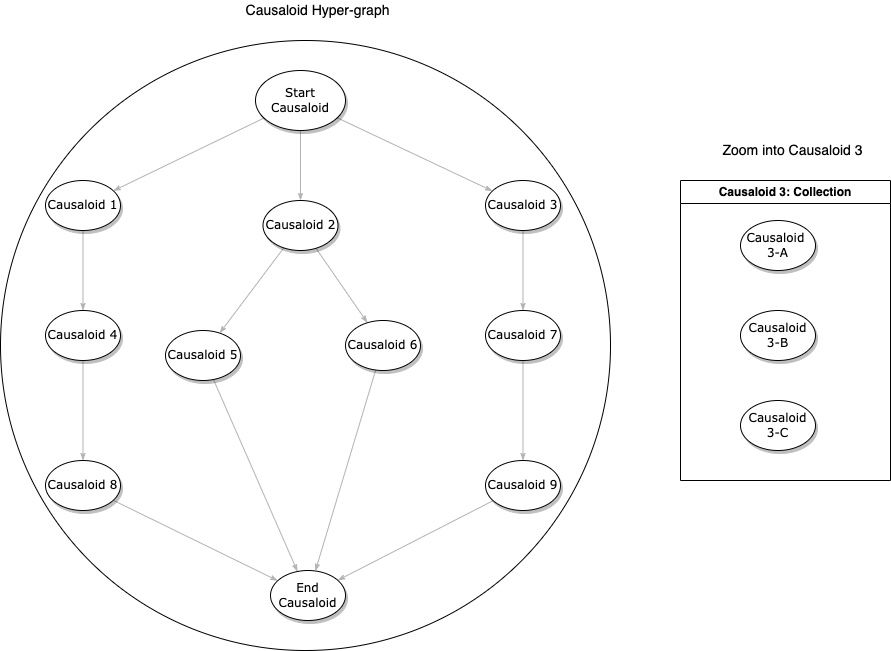
\includegraphics[width=0.8\textwidth]{img/causaloid.png} % Adjust width as needed
    \caption{The Causaloid Diagram illustrating the recursive isomorphic structure of a CausaloidGraph. Nodes within the graph can be elementary Causaloids, collections of Causaloids, or even encapsulate entire sub-\texttt{CausaloidGraphs}, enabling hierarchical and modular causal model construction. }
    \label{fig:causaloid_diagram}
\end{figure}

This recursive definition, as illustrated in Figure~\ref{fig:causaloid_diagram}, allows for a highly modular and hierarchical approach to building complex causal models. Macro-level causal phenomena can be represented by high-level nodes in a graph, and these nodes can then be decomposed into more detailed sub-graphs representing the interacting micro-level causal mechanisms that constitute the higher-level effect. This "transparent composability" \footnote{https://deepcausality.com/docs/concepts} means that a complex system can be broken down into understandable, manageable, and potentially reusable causal modules.

\newpage

Reasoning over a CausaloidGraph involves evaluating its constituent causal elements and propagating their activation states according to the (hyper)edges ($E_G$) that define their logical interdependencies ($\text{logic}_e$). DeepCausality supports various reasoning modes over the graph, such as reasoning over the entire graph, a specific Causaloid node, a defined sub-graph between start and stop nodes, or along the shortest path between two Causaloids. The activation state of a Causaloid (once active, it typically remains so until negatively re-evaluated based on new inputs) allows the graph to maintain a memory of which causal conditions have been met, facilitating reasoning over evolving states based on changing input data and context.

Contextualized causal reasoning is implemented by passing an immutable reference implicitly into the causal function. This mechanism also allows us to contextualize certain Causaloids while leaving others context-free if this is a desirable option. The diagram below, Figure~\ref{fig:contextual_causal_model}, shows this scenario in which specific Causaloids use data from a Context while other Causaloids remain context-free.

\begin{figure}[H] % Or [htbp] for more standard float behavior
    \centering
    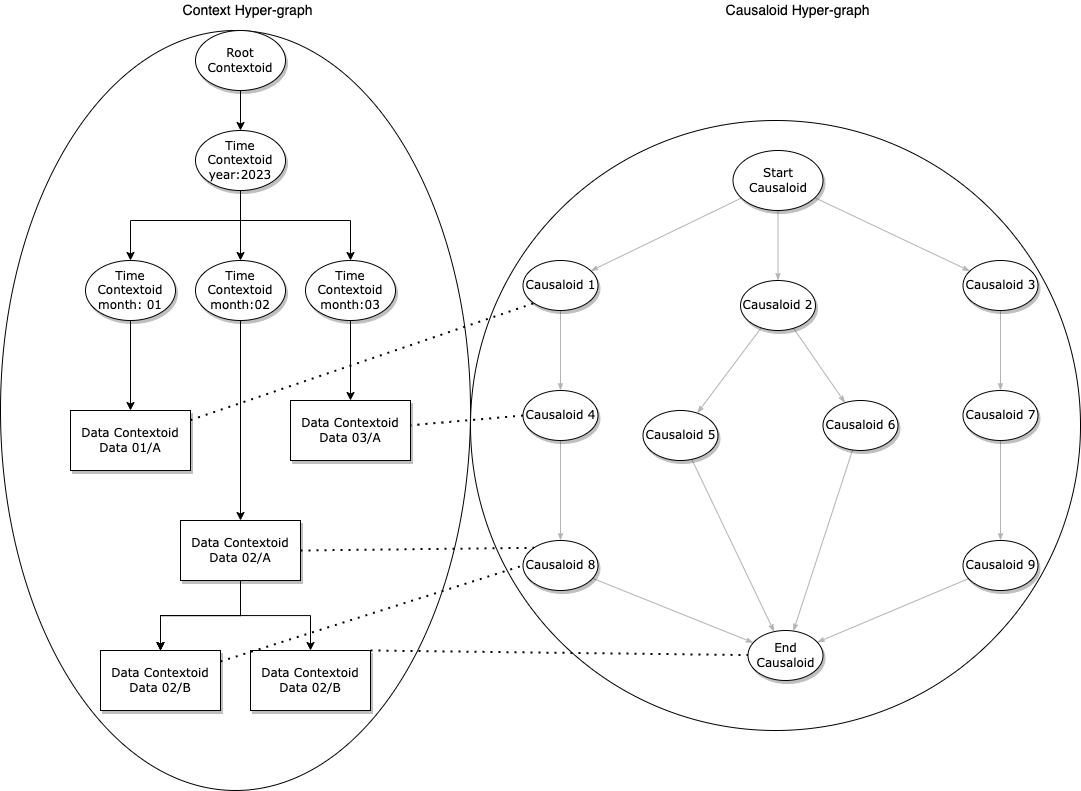
\includegraphics[width=0.9\textwidth]{img/contextual-model.png} % Adjust width as needed
    \caption{Illustration of a Contextual Causal Model in DeepCausality. Specific \texttt{Causaloids} are shown interacting with an external \texttt{Context}  drawing contextual data to inform their evaluation. Other \texttt{Causaloids} operate without direct contextual input, demonstrating the flexibility of selective contextualization.}
    \label{fig:contextual_causal_model}
\end{figure}

This structural approach, combining operational Causaloids with deeply contextualized reasoning and recursively composable CausaloidGraphs, provides DeepCausality with a robust and expressive engine for modeling and executing complex causal knowledge.

\newpage

\subsection{Causal State Machine}
\label{subsec:csm}

A crucial further step for many practical causality based applications is the translation of these causal insights into tangible actions or interventions. The \textbf{Causal State Machine (CSM)} is the component within DeepCausality specifically engineered to bridge this gap, enabling a direct and deterministic linkage from identified causal conditions to predefined operational responses. This facilitates the creation of dynamic control, supervision, and autonomous decision-making systems grounded in explicit causal logic.

The conventional view of causal models often separates the modeling process from subsequent intervention, primarily for reasons of flexibility and analytical clarity. While this separation remains valid and useful for many analytical or exploratory use cases, it can be suboptimal for systems requiring tight, deterministic coupling between causal understanding and immediate action, such as in dynamic control systems or automated supervision. Traditional finite state machines (FSMs), often employed in control systems, typically require all possible system states to be known upfront. However, with the advent of cloud-native applications and other dynamically evolving systems, such as those involving programmatically managed software services or parametric causal models that are brought online and offline dynamically, the complete set of system states may not be known at design time. This limitation restricts the applicability of conventional FSMs.

DeepCausality's CSM offers a more flexible and powerful paradigm. It generalizes the concept of a state machine by defining states not merely as arbitrary system configurations, but specifically as \textit{identified causes} or \textit{combinations of causes} becoming active within one or more supervised CausaloidGraphs. When a particular causal state is recognized through the evaluation of the associated causal model(s) against current observations and context, the CSM is designed to trigger a specific, predefined action or intervention that leads to a desired effect or system adjustment\footnote{https://deepcausality.com/docs/csm}. The core architecture of a CSM in DeepCausality involves this explicit mapping:
\begin{itemize}
    \item \textbf{Causal States}: A state within the CSM corresponds to a specific pattern of activation across one or more Causaloids in the supervised CausaloidGraph(s). This could be a single Causaloid becoming active (e.g., ``Sensor\_Pressure\_Exceeds\_Threshold'') or a more complex logical combination of multiple Causaloid activations (e.g., ``(Smoke\_Detected AND Temperature\_Rising) OR Emergency\_Override\_Signal\_Active'').
    \item \textbf{Deterministic Actions}: Each defined causal state is linked to a deterministic action. These actions are typically implemented as regular Rust functions, which allows for arbitrary complexity. An action could range from simple logging or alerting, to modifying the system's operational parameters, adjusting context variables for downstream models, triggering external API calls, or initiating complex control sequences.
\end{itemize}
A key characteristic of the CSM is its potential for dynamic configuration\footnote{https://deepcausality.com/docs/intro}. Unlike traditional FSMs, a DeepCausality CSM does not necessarily require all possible causal states and their corresponding actions to be enumerated at the initial design phase. Instead, as new components, systems, or causal hypotheses (represented by new Causaloids or CausaloidGraphs) are introduced or come online, their relevant causal states and associated actions can be dynamically registered with the supervising CSM. For instance, if a system being monitored (e.g., an industrial plant) has new sensors added, the causal rules pertaining to these sensors and the actions to be taken upon their triggering specific conditions can be seamlessly integrated into the existing CSM structure. This allows the CSM to adapt and extend its supervisory capabilities as the system it monitors evolves. 

The CSM, therefore, acts as an orchestrator, as formalized in Section \ref{subsubsec:csm_formalism}. It can manage the flow of information by triggering data extraction from relevant Contextoids, ensuring these updates inform the supervised causal models, and then, based on the collective inference drawn (the active causal states), it initiates precise actions. This operational loop facilitates the development of systems that are not only reactive to their environment but can also be proactive if the causal models have predictive capabilities regarding future states. The explicit link between a well-understood causal condition and a defined action enhances the overall system's explainability and trustworthiness; one can clearly trace why a particular action was taken by examining the active causal state that triggered it and the underlying causal logic and contextual data that led to that state's activation. This contrasts significantly with control systems based on opaque machine learning models where the rationale for an action might be obscure.

In summary, the Causal State Machine is a critical component that elevates DeepCausality from a purely analytical framework to one capable of driving direct, reasoned intervention. It provides the necessary mechanisms for building dynamic control and supervision systems that operate on a foundation of explicit, context-aware causal understanding, enabling more robust, adaptable, and explainable automation.

\newpage

\subsection{Formal Specification of DeepCausality} % Changed from \subsection{Formal Specification} for consistency
\label{subsec:formal_specification}

To provide a rigorous underpinning for the conceptual framework described, this section introduces a formal mathematical specification for the core components of DeepCausality, including foundational elements for empirical grounding and assumption management, followed by Context, then Causality types, and the Causal State Machine.

\subsubsection{Foundational Elements: Observation, Assumption, and Inference}
\label{subsubsec:foundational_elements_formalism}

At the base of empirical causal reasoning within DeepCausality are Observations, the Assumptions under which they are interpreted, and the Inference process that links them to causal claims.

An \textbf{Observation Instance}, denoted $o_{data}$, represents a single empirical data point or a collection of related measurements. It is defined primarily by its content:
\[ o_{data} = (id_{obs}, \text{val}_{obs}, \text{eff}_{obs}) \]
where:
\begin{itemize}
    \item $id_{obs} \in \mathbb{I}$ is a unique identifier for the observation, where $\mathbb{I}$ is a suitable set of identifiers.
    \item $\text{val}_{obs} \in \text{NumericalValue}$ (or a more general data type $\mathcal{V}_{obs}$) is the primary measured value associated with a potential causal factor.
    \item $\text{eff}_{obs} \in \text{NumericalValue}$ (or a Boolean/categorical type $\mathcal{V}_{eff}$) is the observed outcome or effect associated with this observation.
\end{itemize}
A dataset typically consists of a set of such observations $D_{obs} = \{o_{data,1}, \dots, o_{data,N}\}$. The Observable trait ensures access to these components.
\newline % Kept your newline for spacing between definitions

An \textbf{Assumption Instance}, denoted $A_{smp}$, articulates a condition believed to hold for a given analysis or context, under which causal interpretations are made. It is defined as:
\[ A_{smp} = (id_{asmp}, \text{desc}_{asmp}, f_{asmp}, \text{status}_{asmp}) \] % Changed state_asmp to status_asmp for consistency with Inference
where:
\begin{itemize}
    \item $id_{asmp} \in \mathbb{I}$ is a unique identifier for the assumption.
    \item $\text{desc}_{asmp}$ is a textual description (e.g., String).
    \item $f_{asmp}$ is the \textbf{assumption evaluation function} (EvalFn):
    \[ f_{asmp}: \mathcal{P}(D_{obs}) \times \text{ContextAccessor}(\mathcal{C}_{\text{relevant}}) \to \{\text{true}, \text{false}\} \]
    This function takes relevant observational data (e.g., a subset of $D_{obs}$, denoted $\mathcal{P}(D_{obs})$ as the power set or a specific subset type) and potentially contextual information from relevant contexts $\mathcal{C}_{\text{relevant}} \subseteq \mathcal{C}_{sys}$, and returns whether the assumption is considered to hold.
    \item $\text{status}_{asmp} = (\text{is\_tested}, \text{is\_valid})$ are Boolean flags indicating the verification status of the assumption.
\end{itemize}
The Assumable trait mandates methods to access these components and to verify the assumption (which executes $f_{asmp}$ and updates $\text{status}_{asmp}$).

\newpage

An \textbf{Inference Instance}, denoted $I_{inf}$, represents a tested hypothesis about a potential causal link, derived from observations under specified assumptions. It is defined as:
\[ I_{inf} = (id_{inf}, \text{question}_{inf}, \text{strength}_{obs}, \text{threshold}_{inf}, \text{effect\_val}_{inf}, \text{target\_val}_{inf}, \text{status}_{inf}) \] % Added subscript inf for clarity
where:
\begin{itemize}
    \item $id_{inf} \in \mathbb{I}$ is a unique identifier.
    \item $\text{question}_{inf}$ is a textual description of the inferential question being posed.
    \item $\text{strength}_{obs} \in [0,1]$ is a numerical value representing the observed strength or probability of the hypothesized relationship, computed from $D_{obs}$ (e.g., derived from $P(E|A)$ and $P(\neg E|\neg A)$ after applying ObservableReasoning).
    \item $\text{threshold}_{inf} \in [0,1]$ is a predefined threshold against which $\text{strength}_{obs}$ is compared.
    \item $\text{effect\_val}_{inf}$ and $\text{target\_val}_{inf}$ are values (of type NumericalValue or similar) used to define the conditions for a positive inference.
    \item $\text{status}_{inf} = (\text{is\_inferable}, \text{is\_inverse\_inferable})$ are Boolean flags. The Conjoint Delta, $\Delta_{CJ}(I_{inf}) = |1 - \text{strength}_{obs}|$, is implicitly defined.
\end{itemize}
The Inferable trait provides methods to access these components and determine $\text{status}_{inf}$. These Inference objects, when validated against Assumptions, form the basis for encoding Causaloids.

\subsubsection{Context Formalism}
\label{subsubsec:context_formalism_main} % Renamed from subsubsec:context_formalism to avoid conflict

A \textbf{System Context Capability} is defined as a finite set of potentially distinct Context Hypergraphs:
\[ \mathcal{C}_{sys} = \{C_1, C_2, \dots, C_k\} \]
where each $ C_i $ is an individual \textbf{Context Hypergraph}.

An individual \textbf{Context Hypergraph} $ C $ is defined as a tuple:
\[ C = (V_C, E_C, ID_C, \text{Name}_C) \]
where:
\begin{itemize}
    \item $ ID_C \in \mathbb{N} $ is a unique identifier for this context within $ \mathcal{C}_{sys} $.
    \item $ \text{Name}_C $ is a descriptive name (e.g., String).
    \item $ V_C $ is a finite set of \textbf{Contextoid} nodes.
    \item $ E_C $ is a finite set of \textbf{Hyperedges}.
\end{itemize}

A \textbf{Contextoid} $ v \in V_C $ is defined as a tuple:
\[ v = (id_v, \text{payload}_v, \text{adj}_v) \]
where:
\begin{itemize}
    \item $ id_v \in \mathbb{I} $ is a unique identifier for the contextoid within $ C $.
    \item $ \text{payload}_v $ is a tagged union:
    \[ \text{payload}_v \in \{ \text{Data}(d) \mid d \in \mathcal{D}_T \} \cup \{ \text{Time}(t) \mid t \in \mathcal{T} \} \cup \{ \text{Space}(s) \mid s \in \mathcal{S} \} \cup \{ \text{SpaceTime}(st) \mid st \in \mathcal{ST} \} \]
    where $\mathcal{D}_T, \mathcal{T}, \mathcal{S}, \mathcal{ST}$ are sets of possible data, temporal, spatial, and spacetime values respectively. Temporal values $t$ are typically $(\text{scale}, \text{unit})$ with $\text{scale} \in \mathcal{T}_{\text{scale}}$ and $\text{unit} \in \mathcal{T}_{\text{unit}}$. Spatial values $s$ are $(x,y,z)$ with coordinates in $T_{coord}$. The interpretation (Euclidean or Non-Euclidean) depends on $T_{coord}$ and the functions defined via the Spatial<V> trait.
    \item $ \text{adj}_v = (\text{update}_v, \text{adjust}_v) $ are optional functions implementing the Adjustable protocol, where $ \text{update}_v: \mathcal{V}_{\text{payload}} \to \text{void} $ and $ \text{adjust}_v: \mathcal{V}_{\text{adj\_factor}} \to \text{void} $.
\end{itemize}

\newpage

A \textbf{Hyperedge} $ e \in E_C $ is a tuple: $ e = (V_e, \text{kind}_e, \text{label}_e) $
where $ V_e \subseteq V_C $ ($|V_e| \ge 1$), $\text{kind}_e \in \mathcal{K}_{\text{relation}}$, and $\text{label}_e$ is optional.

\subsubsection{Causaloid and CausaloidGraph Formalism}
\label{subsubsec:causaloid_graph_formalism}

A \textbf{Causaloid} $ \chi $ is a tuple: $ \chi = (id_\chi, f_\chi, \mathcal{C}_{refs}, \text{desc}_\chi, \mathcal{A}_{linked}, I_{linked}) $
where:
\begin{itemize}
    \item $ id_\chi \in \mathbb{I} $.
    \item $ f_\chi: \mathcal{O}_{\text{type}} \times \text{ContextAccessor}(\mathcal{C}_{refs}) \to \{\text{true}, \text{false}\} $ is the causal function. $\mathcal{O}_{\text{type}}$ is the observation type.
    \item $ \mathcal{C}_{refs} \subseteq \mathcal{C}_{sys} $ are referenced contexts.
    \item $ \text{desc}_\chi $ is a description.
    \item $ \mathcal{A}_{linked} $ (optional) is a set of $id_{asmp}$ for linked Assumptions.
    \item $ I_{linked} $ (optional) is an $id_{inf}$ for the founding Inference.
\end{itemize}

A \textbf{CausaloidGraph} $ G $ is a hypergraph: $ G = (V_G, E_G, ID_G, \text{Name}_G) $
where:
\begin{itemize}
    \item $ V_G $ is a set of causal nodes $v_g = (id_g, \text{payload}_g)$. The payload $\text{payload}_g$ can be a Causaloid $\chi$, a collection $\{\chi_i\}$, or another CausaloidGraph $G'$, reflecting recursive isomorphism.
    \item $ E_G $ is a set of causal hyperedges $e_g = (V_{\text{source}}, V_{\text{target}}, \text{logic}_e)$, where $\text{logic}_e$ defines the functional relationship.
\end{itemize}
The \textbf{state} of $ G $ is $ S_G: V_G \to \{\text{active}, \text{inactive}\} $.

\subsubsection{Causal State Machine (CSM) Formalism}
\label{subsubsec:csm_formalism} 

A \textbf{Causal State Machine} $ M $ is a tuple: $ M = (\mathcal{G}_{M}, \mathcal{C}_{M}, Q, \mathcal{P}_{state}, A, \delta) $
where:
\begin{itemize}
    \item $ \mathcal{G}_{M} = \{G_1, \dots, G_m\} $ are supervised CausaloidGraphs.
    \item $ \mathcal{C}_{M} \subseteq \mathcal{C}_{sys} $ are relevant Context Hypergraphs.
    \item $ Q $ is a finite set of causal states.
    \item $ \mathcal{P}_{state} $ is a set of state activation predicates $ P_q: \prod_{i=1}^{m} \text{StateSpace}(G_i) \to \{\text{true}, \text{false}\} $ for each $q \in Q$.
    \item $ A $ is a finite set of deterministic actions $a: \mathcal{W}_{\text{state}} \to \mathcal{W}_{\text{state}}'$.
    \item $ \delta: Q_{\text{active}} \to A $ is the action triggering function, where $ Q_{\text{active}} = \{ q \in Q \mid P_q(\dots) = \text{true} \} $.
\end{itemize}

A \textbf{Causal State Machine} $ M $ orchestrates actions based on the state of one or more causal models within their contexts. It is defined as a tuple:
$[ M = (\mathcal{G}{M}, \mathcal{C}{M}, Q, P, A, \delta) ]$
where:
\begin{itemize}
\item $ \mathcal{G}{M} = {G_1, G_2, \dots, G_m} $ is the set of CausaloidGraphs supervised by this CSM.
\item $ \mathcal{C}{M} \subseteq \mathcal{C}{sys} $ is the set of Context Hypergraphs relevant to the supervised models and potentially the CSM's state logic.
\item $ Q $ is a finite set of \textbf{causal states}. Each state represents a meaningful condition derived from the activation states of the supervised CausaloidGraphs.
\item $ P $ is a set of \textbf{state activation predicates}. For each state $ q \in Q $, there is a predicate $ P_q $ that 
maps the combined activation states of the supervised graphs to a Boolean value:
$[ P_q: \text{StateSpace}(G_1) \times \dots \times \text{StateSpace}(G_m) \to {\text{true}, \text{false}} ]$
where $ \text{StateSpace}(G_i) $ represents the set of all possible activation mappings $ S{G_i} $. A state $ q $ is active if $ P_q $ evaluates to true. 
\item $ A $ is a finite set of deterministic \textbf{actions}. Each action $ a \in A $ is a function representing an intervention or operation, potentially modifying the environment, the context, or the system state: $ a: \text{WorldState} \to \text{WorldState}' $.
\item $ \delta $ is the \textbf{action triggering function}. It maps active causal states to specific actions:
$ [ \delta: Q_{\text{active}} \to A ]where  Q_{\text{active}} = { q \in Q \mid P_q(\dots) = \text{true} } $. 
Note that multiple states might be active simultaneously, potentially triggering multiple actions based on the CSM's execution semantics (e.g., parallel execution, prioritized execution).
\end{itemize}

\newpage

\subsection{Implementation in Rust}
\label{subsec:rust_implementation}

The conceptual and formal architecture of DeepCausality is concretely realized through a reference implementation in the Rust programming language. This choice was driven by the need for a high-performance, memory-safe, and expressive environment capable of managing the complexities inherent in advanced causal modeling. The Rust implementation translates the abstract concepts of \texttt{Contextoids}, \texttt{Causaloids}, \texttt{CausaloidGraphs}, and Causal State Machines into robust and efficient software components, with a particular emphasis on leveraging Rust's powerful trait system and generics to achieve modularity, extensibility, and type safety. We will highlight key aspects of this implementation, focusing on the \texttt{Causaloid} as the elemental unit of causation and the \texttt{CausaloidGraph} as the structure for composing complex causal models.

\subsubsection{The Causaloid Implementation: Encapsulating Causal Logic}
\label{subsubsec:causaloid_implementation}

The \texttt{Causaloid}, representing an individual causal link or hypothesis, is a central struct in the Rust implementation\footnote{\url{https://github.com/deepcausality-rs/deep_causality/blob/main/deep_causality/src/types/reasoning_types/causaloid/mod.rs}}. It encapsulates an identifier, a description, its current activation state (managed with thread-safe primitives like \texttt{Arc<RwLock<bool>>} for potential concurrent access), and crucially, the causal logic itself.

A key design feature is the \texttt{Causaloid}'s internal \texttt{CausalType} enum\footnote{\url{https://github.com/deepcausality-rs/deep_causality/blob/main/deep_causality/src/types/reasoning_types/causaloid/causal_type.rs}}, which allows a single \texttt{Causaloid} struct to represent one of three distinct structural forms:
\begin{enumerate}
    \item A \texttt{CausalType::Singleton}: This represents an elementary cause, directly holding an optional causal function. This function can be context-free (type \texttt{CausalFn}) or context-aware (type \texttt{ContextualCausalDataFn}), with the latter taking an immutable reference to a \texttt{Context} object.
    \item A \texttt{CausalType::Collection}: This allows a \texttt{Causaloid} to encapsulate an entire collection (e.g., a \texttt{Vec}) of other \texttt{Causaloids}. The evaluation of such a "collection" \texttt{Causaloid} typically involves applying reasoning logic over its constituent members, facilitated by the \texttt{CausableReasoning} trait.
    \item A \texttt{CausalType::Graph}: This enables a \texttt{Causaloid} to encapsulate an entire \texttt{CausaloidGraph} struct, thereby directly realizing the recursive isomorphic nature of the causal modeling engine.
\end{enumerate}
This enum-based design, combined with generic type parameters for context-related data types ($D, S, T, ST, V$), makes the \texttt{Causaloid} struct remarkably versatile. Various constructors are provided to create \texttt{Causaloids} of each \texttt{CausalType}, optionally associating them with specific \texttt{Context} instances if their causal logic is context-dependent.

The behavior of a \texttt{Causaloid} is governed by its implementation\footnote{\url{https://github.com/deepcausality-rs/deep_causality/blob/main/deep_causality/src/types/reasoning_types/causaloid/causable.rs}}  of the \texttt{Causable}\footnote{\url{https://github.com/deepcausality-rs/deep_causality/blob/main/deep_causality/src/protocols/causable/mod.rs}} trait. This trait mandates methods like \texttt{explain()}, \texttt{is\_active()}, \texttt{is\_singleton()}, \texttt{verify\_single\_cause()}, and \texttt{verify\_all\_causes()}. The implementation of these methods for the \texttt{Causaloid} struct intelligently dispatches behavior based on its internal \texttt{CausalType}:
\begin{itemize}
    \item For a \texttt{Singleton}, \texttt{verify\_single\_cause()} executes its stored causal function (either context-free or context-aware).
    \item For a \texttt{Collection}, \texttt{verify\_all\_causes()} delegates to the \texttt{reason\_all\_causes()} method of the encapsulated collection (which benefits from the \texttt{CausableReasoning} extension trait). \texttt{is\_active()} might check if any member of the collection is active.
    \item For a \texttt{Graph}, \texttt{verify\_all\_causes()} delegates to the \texttt{reason\_all\_causes()} method of the encapsulated \texttt{CausaloidGraph} (which benefits from the \texttt{CausableGraphReasoning} trait).
\end{itemize}
This elegant delegation ensures that a \texttt{Causaloid}, regardless of its internal complexity (simple function, collection, or entire graph), presents a uniform interface to the rest of the system, particularly when it is itself a node within a higher-level \texttt{CausaloidGraph}.

\newpage

\subsubsection{The CausaloidGraph Implementation: Composing and Reasoning Over Causal Networks}
\label{subsubsec:causaloidgraph_implementation}

The \texttt{CausaloidGraph} is the primary structure for composing multiple \texttt{Causaloids} into complex causal networks. In the Rust implementation, this is realized as a generic struct, \texttt{CausaloidGraph<T> where T: Causable + PartialEq}, which internally uses a graph data structure (specifically, an \texttt{UltraGraph<T>}\footnote{\url{https://github.com/deepcausality-rs/deep_causality/tree/main/ultragraph}}) to store \texttt{Causable} nodes and their relationships. The power and ergonomics of the \texttt{CausaloidGraph} implementation are significantly enhanced by a layered trait design:
\begin{enumerate}
    \item \textbf{Base Graph Operations via \texttt{CausableGraph<T>}}\footnote{\url{https://github.com/deepcausality-rs/deep_causality/blob/main/deep_causality/src/protocols/causable_graph/graph.rs}}: This trait provides the fundamental Application Programming Interface (API) for graph manipulation, such as adding or removing \texttt{Causaloid} nodes and edges, checking for their existence, managing a root node, and retrieving graph metrics like size and number of active nodes. A crucial method in this trait is \texttt{get\_graph(\&self) -> \&CausalGraph<T>}, which returns a reference to the underlying graph data structure (the \texttt{UltraGraph} instance). This accessor is key to enabling default implementations in higher-level traits. The \texttt{impl CausableGraph<T> for CausaloidGraph<T>} block provides the concrete logic for these operations, typically by delegating to the methods of the underlying \texttt{UltraGraph}.

    \item \textbf{Defaulted Reasoning Logic via \texttt{CausableGraphReasoning<T>}}\footnote{\url{https://github.com/deepcausality-rs/deep_causality/blob/main/deep_causality/src/protocols/causable_graph/graph_reasoning.rs}}: This trait extends \texttt{CausableGraph<T>} by providing a suite of sophisticated reasoning methods, such as \texttt{reason\_all\_causes()}, \texttt{reason\_subgraph\_from\_cause()}, \texttt{reason\_shortest\_path\_between\_causes()}, and \texttt{reason\_single\_cause()}. Critically, these methods are provided with \textit{default implementations} directly within the trait definition (or are implemented in a blanket way for any type that implements \texttt{CausableGraph<T>}). These defaults leverage the \texttt{get\_graph()} accessor to operate on the graph structure and call the \texttt{Causable} trait methods (like \texttt{verify\_single\_cause}) on the individual \texttt{Causaloid} nodes. For instance, \texttt{reason\_from\_to\_cause()} implements a depth-first-search-like traversal, verifying each \texttt{Causaloid} along the path using observation data. Users of \texttt{CausaloidGraph} automatically receive this rich reasoning functionality simply because \texttt{CausaloidGraph<T>} implements trait \texttt{CausableGraph<T>}.

    \item \textbf{Defaulted Explaining Logic via \texttt{CausableGraphExplaining<T>}}\footnote{\url{https://github.com/deepcausality-rs/deep_causality/blob/main/deep_causality/src/protocols/causable_graph/graph_explaining.rs}}: Similar to reasoning, this trait extends \texttt{CausableGraph<T>} and provides default implementations for methods like \texttt{explain\_all\_causes()} and \texttt{explain\_shortest\_path\_between\_causes()}. These methods traverse the graph (again, using \texttt{get\_graph()}) and aggregate the string explanations obtained by calling the \texttt{explain()} method on each constituent \texttt{Causaloid}.
\end{enumerate}
This strategic use of traits with default implementations, relying on a minimal set of required methods in a base trait (\texttt{CausableGraph<T>} requiring \texttt{get\_graph()}), dramatically reduces code duplication and complexity. It means that the sophisticated logic for graph traversal, data mapping, and aggregation for both reasoning and explaining only needs to be written once, within the default trait methods. Any specific graph structure that correctly implements the basic \texttt{Causaloid} storage and access via \texttt{CausableGraph<T>} can instantly inherit this full suite of advanced capabilities. This is a powerful demonstration of Rust's ability to build highly abstract yet efficient and maintainable systems, significantly lowering the implementation burden for complex functionalities. The clear separation of concerns—basic graph structure, reasoning logic, and explaining logic, each in its own trait—further enhances modularity and testability.

The concrete realization of these causal graph structures within DeepCausality utilizes \texttt{UltraGraph}\footnote{\url{https://github.com/deepcausality-rs/deep_causality/tree/main/ultragraph}}, a custom-developed Rust graph library designed to provide an ergonomic API layer over robust underlying graph representations. \texttt{UltraGraph} leverages the hypergraph capabilities of the \texttt{petgraph} crate, specifically employing an adjacency matrix-based graph structure from \texttt{petgraph} to represent the network of \texttt{Causaloids} and their potentially N-ary relationships (hyperedges). To facilitate efficient node management and direct access, \texttt{UltraGraph} typically combines this with a \texttt{HashMap} for storing the \texttt{Causaloid} nodes themselves, keyed by their identifiers. This approach allows DeepCausality to benefit from \texttt{petgraph}'s foundational graph algorithms and data structures while offering a simplified and more specific interface for causal modeling tasks, including methods for direct node retrieval, neighbor access, and shortest path calculations. The \texttt{impl CausableGraph<T> for CausaloidGraph<T>} block then implements DeepCausality's specific graph operations by interfacing with these \texttt{UltraGraph} capabilities.

\newpage

\subsubsection{The Context Implementation: Traits, Generics, and Hypergraphs}
\label{subsubsec:context_engine_implementation}

The Context architecture relies on the language's powerful trait system and generics to manage diverse contextual data types and their interactions within a hypergraph structure, while ensuring type safety and enabling extensibility. This design facilitates a clean and idiomatic separation between immutable and mutable contextual elements, a key factor in ensuring both data integrity and adaptability.

At the foundation are several elemental traits, primarily defined in the conceptual module for context nodes\footnote{\url{contextuable.txt}}, which establish the contracts for different kinds of contextual information. The Datable trait marks identifiable data-holding entities. More specialized traits include Temporable<V>, for objects possessing a time scale and unit (with TimeScale being a dedicated enum\footnote{\url{time_scale.txt}}); Spatial<V>, for those with up to three spatial coordinates (X, Y, Z) of a generic numeric type V; and SpaceTemporal<V>, which combines both spatial and temporal properties, also providing access to a temporal coordinate t. The generic parameter V for these traits is constrained with standard Rust operational traits (e.g., Default, Copy, Clone, Hash, Eq, arithmetic operations) ensuring that dimensional values are workable and can represent a wide range of numeric types suitable for diverse geometric interpretations, including both Euclidean and non-Euclidean spaces.

Concrete instantiations of these concepts are provided as distinct Rust structs. For example, an immutable temporal node is represented by Time<T>\footnote{\url{time.txt}}, a spatial node by Space<T>\footnote{\url{space.txt}}, a combined spatio-temporal node by SpaceTime<T>\footnote{\url{sapce_time.txt}}, and a general data-holding node by Data<T>\footnote{\url{data.txt}}. Each of these structs implements its corresponding elemental trait (e.g., impl Temporable<T> for Time<T>). These structs often utilize procedural macros like deep\_causality\_macros::Constructor and Getters for ergonomic instance creation and field access.

To handle evolving environments where contextual information must change, DeepCausality provides distinct Adjustable counterparts for these node types, such as AdjustableTime<T>\footnote{\url{adjutable_time.txt}} and AdjustableSpaceTime<T>\footnote{\url{adjustable_space_time.txt}}. These structs implement the Adjustable<T> trait\footnote{\url{adjustable.txt}}, which defines optional update and adjust methods. These methods take an ArrayGrid as an argument, providing a structured way to pass new values or transformation parameters. For instance, the impl Adjustable<T> for AdjustableTime<T> demonstrates how an incoming 1D ArrayGrid value is used to either replace (update) or modify (adjust) the internal time\_unit, along with necessary validation checks (e.g., ensuring time does not become negative). Similarly, the implementation for AdjustableSpaceTime<T> uses a 4D PointIndex to extract new x, y, z, and time values from the ArrayGrid for updates or adjustments. This explicit separation between immutable and adjustable types ensures that mutability is an opt-in feature, enhancing the predictability and safety of context management.

The Contextoid<D,S,T,ST,V> struct\footnote{\url{contextoid.txt}} serves as a generic wrapper, encapsulating a unique identifier and a ContextoidType<D,S,T,ST,V> enum\footnote{\url{contextoid_type.txt}}. This enum acts as a tagged union, holding one of the concrete dimensional struct instances (e.g., Datoid(Data<MyPayloadType>), Tempoid(AdjustableTime<MyTimeUnit>), Spaceoid(Space<MyCustomNonEuclideanCoord>)). The Contextoid itself then implements the overarching Contextuable<D,S,T,ST,V> trait\footnote{The impl Contextuable for Contextoid is defined in \url{contextuable.txt} which appears to be part of the Contextoid module structure.}, providing a uniform interface (e.g., via the vertex\_type() method) regardless of the specific dimensional data it holds. This design allows a ContextHypergraph to store heterogeneous Contextoid types while still enabling type-safe access and efficient static dispatch through pattern matching on the ContextoidType enum.

The overall organization of Contextoids and their interrelationships is managed by the main Context<D,S,T,ST,V> struct\footnote{\url{context_graph.txt}}. This struct acts as the primary container, holding a base\_context (typically an UltraGraph<Contextoid<...>> instance for the default context) and, optionally, an extra\_contexts field (e.g., a HashMap<u64, UltraGraph<Contextoid<...>>>) to manage multiple, uniquely identifiable context hypergraphs.

The base\_context and each of the extra\_contexts within the main Context struct are implemented as instances of a hypergraph data structure. This is also built upon the UltraGraph library, which, by utilizing the underlying hypergraph support of the petgraph crate (specifically its adjacency matrix graph implementation), provides the necessary foundation for representing Contextoids as nodes and their N-ary contextual relationships as hyperedges. This choice ensures efficient storage and access mechanisms for Contextoids and their complex interdependencies. The methods defined in the ContextuableGraph and ExtendableContextuableGraph traits are then implemented by the Context struct, leveraging these UltraGraph functionalities to manipulate the respective context hypergraphs.

The Context struct then implements the ContextuableGraph<D,S,T,ST,V> trait for operations on the base context, and the ExtendableContextuableGraph<D,S,T,ST,V> trait (both defined in the contextuable\_graph trait file\footnote{\url{contextuable_graph.txt}} but likely with concrete implementations for the Context struct in files like \url{contextuable_graph.txt} and \url{extendable_contextuable_graph.txt} located within the Context struct's module) for managing and interacting with these additional contexts. These traits define a clean API for adding, removing, and querying nodes (Contextoids) and edges (which are typed with a RelationKind enum\footnote{\url{relation_kind.txt}}) within the selected context hypergraph. The extensive use of generics ($D, S, T, ST, V$) throughout these definitions allows users to integrate their own specific data types for observations, time units, and spatial coordinates, facilitating the framework's adaptability to diverse domains and geometric representations, including sophisticated non-Euclidean models. This meticulous, trait-driven, and generically-typed implementation in Rust culminates in a uniquely expressive, performant, and robust system for deeply contextualized causal reasoning.

\subsubsection{The Causal State Machine Implementation: Linking Causes to Actions}
\label{subsubsec:csm_implementation}

The Causal State Machine (CSM) is a critical component in DeepCausality that operationalizes causal inferences by translating identified causal conditions into deterministic actions. Its Rust implementation focuses on providing a flexible yet robust mechanism for defining states based on Causaloid activations and linking these states to user-defined functions representing interventions or responses.

At the core of the CSM are two primary structs: \texttt{CausalAction} and \texttt{CausalState}. A \texttt{CausalAction}\footnote{\url{csm_action.txt}} is a straightforward struct encapsulating a function pointer (\texttt{action: fn() -> Result<(), ActionError>}), a textual description, and a version. The \texttt{fire()} method simply invokes this function pointer, allowing any Rust function adhering to the specified signature to serve as an action. This provides maximal flexibility for defining complex interventions.

% Suggested Code Listing: CausalAction Definition
\begin{lstlisting}[label={list:csm_action_def}, caption={Conceptual Definition of \texttt{CausalAction} in Rust.}]
// (simplified for illustration)
pub struct CausalAction {
    action: fn() -> Result<(), ActionError>,
     descr: &'static str,
     // ... other fields
}

impl CausalAction {
     pub fn fire(&self) -> Result<(), ActionError> {
         (self.action)()
     }
}

// Example Action Function:
fn log_critical_pressure_action() -> Result<(), ActionError> {
    println!("CRITICAL ACTION: Pressure threshold exceeded!");
    Ok(())
}
// let critical_pressure_action = CausalAction::new(log_critical_pressure_action, "Logs critical pressure", 1);
\end{lstlisting}

A CausalState\footnote{\url{csm_state.txt}} represents a specific condition that the CSM monitors. It is generically typed over the same context-related types as Causaloid ($D, S, T, ST, V$) because it directly holds a reference to a Causaloid (\texttt{causaloid: \&'l Causaloid<\&'l, ...>}). 
Additionally, it stores an \texttt{id}, a \texttt{version}, and specific \texttt{data: NumericalValue} against which its associated Causaloid will be evaluated. The CausalState provides evaluation methods: \texttt{eval()} (which uses its stored data) and \texttt{eval\_with\_data(\&self, data: \&NumericalValue)} (which uses externally provided data). 
Both methods ultimately call \texttt{self.causaloid.verify\_single\_cause(...)}, thus linking the CSM's state evaluation directly to the core causal reasoning logic of a Causaloid. 
A state is considered active if its Causaloid evaluates to true for the given data.

% Suggested Code Listing: CausalState Definition
\begin{lstlisting}[label={list:csm_state_def}, caption={Conceptual Definition of \texttt{CausalState} in Rust.}]
// From csm_state.txt (simplified for illustration)
// pub struct CausalState<'l, D, S, T, ST, V>
// where D: Datable + Clone, /* ... other bounds ... */ {
//     id: usize,
//     data: NumericalValue, // Data used for this specific state's Causaloid evaluation
//     causaloid: &'l Causaloid<'l, D, S, T, ST, V>,
//     // ... other fields
// }

// impl<'l, D, S, T, ST, V> CausalState<'l, D, S, T, ST, V>
// where D: Datable + Clone, /* ... other bounds ... */ {
//     pub fn eval(&self) -> Result<bool, CausalityError> {
//         self.causaloid.verify_single_cause(&self.data)
//     }
// }

// Assuming q_pressure_high is a Causaloid that checks for high pressure
// let pressure_state_data: NumericalValue = 150.0; // Specific data for this state
// let state_high_pressure = CausalState::new(
//     state_id_1, 
//     1, // version
//     pressure_state_data, 
//     &q_pressure_high 
// );
\end{lstlisting}

The \texttt{CSM}\footnote{\url{https://github.com/deepcausality-rs/deep_causality/blob/main/deep_causality/src/types/csm_types/mod.rs}} struct itself orchestrates these components. It internally stores a collection of state-action pairs, typically within a \texttt{RefCell<HashMap<usize, (\&'l CausalState<...>, \&'l CausalAction)>>}. The \texttt{RefCell} provides interior mutability, allowing the CSM to add, remove, or update states even when the \texttt{CSM} instance itself is immutably borrowed (a common pattern for shared access in more complex systems). The \texttt{HashMap} allows for efficient lookup of state-action pairs by the state's ID.

The constructor \texttt{CSM::new(state\_actions: \&'l CSMStateActions<...>)} takes an array slice of state-action tuples and populates the internal map. Methods like \texttt{add\_single\_state}, \texttt{remove\_single\_state}, and \texttt{update\_single\_state} allow for the dynamic configuration of the CSM at runtime, as emphasized in Section~\ref{subsec:csm}.

Evaluation is performed via methods like \texttt{eval\_single\_state(id, data)} and \texttt{eval\_all\_states()}. The \texttt{eval\_single\_state} method retrieves the specified \texttt{CausalState} and its associated \texttt{CausalAction}. It then calls the \texttt{eval\_with\_data()} method of the \texttt{CausalState}. If this evaluation returns true (indicating the causal condition for that state is met), the \texttt{fire()} method of the linked \texttt{CausalAction} is invoked. The \texttt{eval\_all\_states()} method iterates through all registered state-action pairs, evaluates each state using its internally stored data, and fires actions accordingly. This design ensures a deterministic link: if a specific causal state (defined by a \texttt{Causaloid} and its input data) is active, its designated action is triggered. The generics ($D, S, T, ST, V$) propagate through these structures, ensuring type consistency from context data through Causaloid evaluation to CausalState definition.
%% Section 5: Advanced Modeling with DeepCausality 
\section{Advanced Modeling with DeepCausality}
\label{sec:advanced_modeling}

The foundational components of DeepCausality—its expressive Context Engine, composable Causal Modeling Engine, and action-oriented Causal State Machines—collectively enable a range of sophisticated modeling paradigms. These paradigms allow for the representation and analysis of systems with intricate contextual dependencies, evolving causal structures, and complex temporal dynamics. This section explores these advanced modeling capabilities, demonstrating how DeepCausality moves beyond static, simplistic causal representations towards a more nuanced and adaptive understanding of cause and effect in real-world systems. We will delve into advanced context modeling techniques, the construction of dynamic and hybrid causal models, and culminate in a discussion of emergent causality, where the causal rules themselves can adapt in response to their operational environment.

\subsection{Advanced Context Modeling}
\label{sucsec:context_modeling}

DeepCausality's context distinguishes between Static Contexts and Dynamic Contexts. This distinction is pivotal, carrying substantial implications for model architecture, system efficiency, and the class of causal problems the system can effectively address.
In a Static Context, the entire topology of the Context Hypergraph—encompassing the defined types of Contextoids, their specific interconnections via hyperedges, and the overall relational schema of the contextual landscape—is established a priori and remains invariant throughout the system's operational phase. While this structural immutability is a defining feature, it is crucial to understand that the values encapsulated within individual Contextoids are generally expected to change. For instance, a Data Contextoid representing a "current-position" in a drone model will be continually updated with new values representing the position, yet its predefined role and its connections to other temporal or instrument-specific Contextoids within the static graph structure will persist. The documentation \footnote{https://deepcausality.com/docs/concepts/} explicitly states, "The context structure is defined beforehand for a static context..." and that for such fixed structures, "...only values stored in it get updated". This paradigm is particularly advantageous in scenarios where the contextual variables impacting a causal system and their interdependencies are well-understood and exhibit long-term stability. The primary benefits are enhanced computational efficiency and predictability. Static structures permit optimized query paths and memory layouts, as noted by the assertion that this approach is more memory efficient. Such contexts are ideal for domains like established industrial process control, where sensor networks are fixed. Even within such structurally static environments, the Adjustable protocol\footnote{https://deepcausality.com/docs/concepts/} remains applicable to individual Contextoids, allowing their internal data to be modified through update() or adjust() operations without necessitating any alteration to the overarching graph topology.

Conversely, Dynamic Contexts offer a paradigm of structural plasticity, wherein the very architecture of the Context Hypergraph can be algorithmically generated, augmented, or pruned during runtime. This implies the capacity to introduce novel Contextoid types, forge new relational hyperedges, or modify existing structural components as the system interacts with and learns from its operational environment. The documentation\footnote{https://deepcausality.com/docs/concepts/} confirms this by stating, "...whereas for a dynamic context, the structure is generated dynamically at runtime," thereby enabling "more dynamic and self-adaptable designs". This capability is indispensable for systems deployed in open-world, non-stationary environments where not all contextual factors can be anticipated at design time. Consider applications such as autonomous robotic exploration of uncharted territories; as the robot encounters new environmental features or objects, it can dynamically instantiate new Contextoids (e.g., representing a newly mapped spatial region or a previously unidentified object type) and integrate them into its evolving contextual model. Similarly, modeling influence in evolving social networks, where participants and relationships frequently change, necessitates a dynamic contextual framework. The implicit potential for dynamic sensor integration in an IoT network, such as incorporating data from a temporary drone inspection service into an existing industrial monitoring system.

The provision for both static and dynamic contextual paradigms recognizes that different problem domains and operational requirements call for different trade-offs between structural stability (and its attendant efficiencies) and structural adaptability (and its capacity to handle novelty and environmental drift). A hybrid approach, where stable, well-understood contextual facets are modeled statically while more volatile or exploratory aspects leverage dynamic sub-contexts, is also implicitly supported by the framework's modular design. The underlying hypergraph representation serves as a versatile structural primitive capable of accommodating both modes of operation, allowing engineers to tailor the contextual grounding of their causal models precisely to the demands of the application at hand.

\subsubsection{Static Context}
\label{subsubsec:adv_static_context}
% Summary: Discuss benefits for well-defined systems, performance advantages.
% How the Adjustable Protocol still allows value dynamism.
% Examples where this is optimal.

\subsubsection{Dynamic Context}
\label{subsubsec:adv_dynamic_context}
% Summary: Discuss benefits for open-world, non-stationary environments.
% How structural plasticity is achieved. Challenges (pruning, query complexity).
% Examples: robotic exploration, evolving social networks.

\subsubsection{Hybrid Static/Dynamic Context Architectures}
\label{subsubsec:adv_hybrid_static_dynamic_context}
% Summary: Explain the concept of partitioning a system's context into stable (static)
% and volatile (dynamic) sub-contexts. How DeepCausality's multi-context or
% modular graph features can support this. Benefits for complex systems where
% some aspects are known and others are exploratory. Example.

\subsubsection{Heterogeneous Euclidean and Non-Euclidean Context Integration}
\label{subsubsec:adv_hybrid_geo_context}
% Summary: Discuss the power of combining different geometric representations within
% a single causal analysis. How Causaloids can query and integrate information
% from both physical (Euclidean) and abstract relational (non-Euclidean) contexts.
% Example: urban planning with physical layout and social network data.
% Link to how this enables modeling richer, more realistic causal influences.

\subsubsection{Multiple, Heterogeneous Hybrid Contexts}
\label{subsubsec:adv_multiple_hybrid_contexts}
% Summary: Intro: Building upon the ability to define contexts that are internally
% hybrid (static/dynamic or Euclidean/non-Euclidean), DeepCausality's support
% for multiple, distinct Context Hypergraphs allows for an even greater level of
% modeling sophistication. This subsection explores how systems can be architected
% to simultaneously leverage several specialized contexts, each potentially
% exhibiting its own hybrid characteristics, to inform a unified causal model.

% A) Orchestrating Diverse Information Sources:
%    - Discuss how a primary CausaloidGraph can be designed to query multiple,
%      concurrently active Context instances.
%    - Example: A global risk assessment model that queries:
%        - Context_GeoPolitical: Non-Euclidean graph of international relations (dynamic structure).
%        - Context_Economic: Time-series data of market indicators (Euclidean, dynamic values).
%        - Context_Climate: Spatial grid of climate model outputs (Euclidean, dynamic values).
%        - Context_PolicyDB: Static database of existing regulations (structured data).
%    - How a single Causaloid's function can synthesize these varied inputs.

% B) Modular Context Management and Domain Expertise:
%    - Reiterate how the multi-context feature allows different domain experts or system
%      modules to manage and update their specific contextual realms independently.
%    - Example: In a smart city application, the transportation department manages a
%      dynamic, Euclidean context of traffic flow, while the social services department
%      manages a non-Euclidean context of community engagement networks. A central
%      urban planning CausaloidGraph queries both.

% C) Enabling Complex Inter-Contextual Causal Links:
%    - Discuss the potential for Causaloids to not only read from multiple contexts
%      but also for the state of one context to influence another (potentially via CSM actions
%      that update Contextoids in a different context graph).
%    - This allows modeling feedback loops or cascading effects that span across
%      different types of contextual information (e.g., how a change in a non-Euclidean
%      social sentiment context might causally impact behaviors observed in a Euclidean
%      economic activity context).

% D) Advantages for Robustness and Nuance:
%    - How this multi-hybrid approach allows for an exceptionally nuanced representation
%      of complex real-world systems, where different facets of reality have different
%      stabilities (static/dynamic) and different relational structures (Euclidean/non-Euclidean).
%    - This leads to causal models that are more robust because they can draw upon and
%      appropriately weight information from a wider, more diverse, and more faithfully
%      represented set of environmental factors.

\newpage

\subsection{Advanced Causality Modeling}
\label{sucsec:causality_modeling}

While the Context Engine (Section~\ref{sucsec:context_modeling}) provides the rich, evolving environmental grounding, the essence of DeepCausality lies in its capacity to construct and reason with explicit causal models that operate upon this context. The Causal Modeling Engine, built around operational Causaloids and recursively composable CausaloidGraphs (as detailed in Section~\ref{sec:deep_causality}), offers significant flexibility in how these causal structures are defined and how they adapt to or interact with temporal dynamics and diverse contextual geometries. This subsection delves into advanced paradigms for causality modeling within DeepCausality, moving beyond simple, static representations. We explore the construction of static causal models for well-defined mechanisms, the principles behind dynamic causal models where the causal structure itself can adapt in response to context, the nuances of dynamic temporal causal reasoning with multi-scale context, and the power of leveraging hybrid (Euclidean/non-Euclidean) contexts and hybrid static/dynamic architectures to create more faithful and adaptive representations of causal reality. These advanced capabilities aim to equip intelligent systems with a more profound and flexible understanding of the generative mechanisms at play in complex environments.

\subsubsection{Static Causal Models}
\label{subsubsec:adv_static_causal_model}
% Summary: Discuss when a fixed CausaloidGraph topology is appropriate.
% Focus on how dynamic context values activate different paths within this fixed structure.
% Example: a well-understood manufacturing process with known failure modes.

\subsubsection{Dynamic Causal Models}
\label{subsubsec:adv_dynamic_causal_model}
% Summary: Introduce the concept that the CausaloidGraph structure itself
% (nodes/Causaloids, edges/dependencies) can be subject to change.
% How context can trigger the generation, selection, or modification of Causaloids
% or parts of the CausaloidGraph. This is where the `dyncaus.txt` ideas start.
% This directly addresses AI's failure in novel environments by allowing the "rules" to change.

\subsubsection{Dynamic Causal Models via (Multiple), Heterogeneous Hybrid Contexts}
\label{subsubsec:adv_dynamic_causal_model_multiple_contexts}
\newpage

\subsubsection{Dynamic Temporal Causal Reasoning}
\label{subsec:temporal_graph_reasoning}

A significant challenge in applying causal reasoning to dynamic systems is the effective and efficient handling of temporal information. Traditional time series analysis often employs sliding window approaches or auto-regressive models where the computational cost or model complexity can scale with the length of the historical data considered. DeepCausality offers an alternative perspective, particularly when the primary causal structure (\textit{i.e.}, the set of causal mechanisms and their interdependencies represented by the CausaloidGraph) is assumed to be stable over time, even if the contextual data it operates upon is highly dynamic.

The core insight involves the interaction between a structurally stable CausaloidGraph and a dynamically updated Context Hypergraph. This Context Hypergraph is not merely a linear sequence of events; it explicitly represents temporal information at multiple, user-defined scales via Time and SpaceTime Contextoids, each associated with a specific TimeScale enum (e.g., Year, Month, Day, Hour, Minute, Second, Nanosecond)\footnote{\url{time_scale.txt}}. At each discrete data sampling interval, new observations update the relevant Contextoids at the appropriate scales within the Context Engine.

When the CausaloidGraph is subsequently evaluated, its constituent Causaloids can query the Context Engine for the \textit{current} state of these Contextoids at any of the modeled time scales. A single causal function $f_\chi$ might simultaneously access ``last\_price\_tick\_at\_nanosecond\_resolution'', ``average\_price\_last\_minute'', and ``volatility\_last\_hour'' by querying distinct Contextoids, each representing a different temporal granularity or aggregation. The causal functions then operate on this rich, multi-scale, time-synchronous contextual data.

The crucial point is that if the topology of the CausaloidGraph itself---the set of Causaloids ($V_G$) and their relational (hyper)edges ($E_G$)---does not change from one time step to the next, then the computational complexity of traversing this graph to perform a reasoning task remains constant, denoted as $O(k)$ where $k$ is a function of $|V_G|$ and $|E_G|$. Access to different time scales within the Context Engine is typically managed via efficient lookups (e.g., using the TimeIndexExt with HashMaps as described in the implementation of CustomContext\footnote{\url{time_index.txt}} and Context\footnote{\url{indexable.txt}}), allowing for near-instantaneous retrieval of contextual data at the required granularity. This direct, indexed access to variable time scales without re-computation or complex windowing logic across the entire history for each query is a distinctive feature.

This architecture offers constant-time graph traversal characteristics for the causal reasoning logic \textit{per evaluation cycle}, irrespective of the raw history length, because the history and its multi-scale aggregations are encapsulated and managed within the Context Engine. The CausaloidGraph operates on the "present moment" as defined by the current state of its accessible, multi-scale contexts. This approach facilitates a non-linear conceptualization of time's influence:
\begin{enumerate}
    \item Time as Explicit, Multi-Scale Context: Time itself is not just a sequence but a structured entity within the Context Hypergraph, modeled via Time or SpaceTime Contextoids that are explicitly aware of their TimeScale. Causal functions can directly query Contextoids representing phenomena at, for example, the second, hour, and day scale simultaneously.
    \item History Encapsulated in Contextual State at Relevant Scales: The influence of the past is summarized or reflected in the current state of other Data Contextoids, potentially maintained at various aggregations. The causal model reasons based on these relevant historical summaries, not by directly traversing an infinitely long chain of past raw events within its own structure. The Adjustable protocol allows these summary Contextoids to be updated efficiently.
    \item Non-Linear Causal Functions: The causal functions within Causaloids ($f_\chi$) can be arbitrarily complex non-linear functions, modeling how the \textit{same} causal mechanism responds differently to varying contextual inputs, including information from different temporal scales provided by the Context Engine.
\end{enumerate}
This architecture allows for a nuanced understanding of time's influence. Instead of a purely linear, chain-like dependence on all past states, time's influence is mediated through a structured, multi-scale Context Engine. The CausaloidGraph remains structurally lean and performant for reasoning, while the Context Engine manages the complexity of temporal data, its historical aggregation, and its presentation at variable scales. The separation of concerns—stable causal logic in the CausaloidGraph and dynamic, multi-scale environmental state in the Context Hypergraph—is key to this efficiency and flexibility.

\subsubsection{Hybrid Contexts for Causal Models}
\label{subsubsec:adv_hybrid_context_for_causality}
% Summary: Specifically discuss how Causaloids operating with both Euclidean and
% non-Euclidean contextual inputs can model more complex causal conditions.
% Example: a Causaloid whose activation depends on both a physical sensor reading (Euclidean)
% and the state of an abstract conceptual category (non-Euclidean).

\subsubsection{Hybrid Static/Dynamic Causal Models}
\label{subsubsec:adv_hybrid_static_dynamic_causal_model}
% Summary: Discuss models where a core, stable set of causal mechanisms (static part of
% CausaloidGraph) interacts with dynamically generated/adapted causal sub-modules.
% Example: A base diagnostic system with pluggable, context-specific diagnostic Causaloids.

\newpage

\subsection{Emergent Causality Modeling}
\label{subsec:emergent_causality}

% Intro: Basics - Define "emergent causality" in the context of DeepCausality:
% the phenomenon where new causal relationships or entire causal structures
% arise or are significantly modified based on the evolving state of the system
% and its context, often in ways not explicitly pre-programmed for every specific
% contingency. This is about the system adapting its *causal understanding*.
% Link this directly to addressing the AI limitation of failing in novel environments
% where the underlying generative process shifts.

The preceding discussions on advanced context and causality modeling with DeepCausality have primarily focused on systems where either the contextual data evolves, or where predefined causal models operate upon this dynamic context. However, the architectural principles of the framework—particularly the operational nature of Causaloids, the composability of CausaloidGraphs, the dynamic Context Engine, and the orchestrating power of Causal State Machines—collectively enable a more profound paradigm: \textit{emergent causality}. This refers to scenarios where not only the states and parameters of a causal model adapt, but where the very structure of the causal model itself can be generated, modified, or selected dynamically in response to the evolving operational context.

This capability moves beyond simulating systems with predefined, albeit complex, causal relationships, towards simulating systems that can adapt their understanding of causality or where new causal mechanisms can effectively "emerge" as the environment changes. It directly addresses a fundamental limitation of many AI systems: their inability to cope with truly novel situations or shifts in the underlying generative process where the old "rules of the game" no
longer apply. In DeepCausality, the "rules of the game" (the active CausaloidGraph) can change based on the "state of the game" (the Context). This allows for systems that can exhibit structural adaptation, simulate forms of innovation or novelty, and even manage the lifecycle of their own causal components.

This section explores how DeepCausality's architecture provides the foundation for modeling such emergent causal phenomena. We will examine the pivotal role of rich, hybrid (Euclidean and non-Euclidean) contexts in triggering these structural adaptations, the function of Causal State Machines in orchestrating the selection or generation of new causal logic, and the conceptual mechanisms by which new causal structures (Causaloids or CausaloidGraphs) can be instantiated "on-demand" based on contextual cues. While the design of specific "causaloid generator functions" remains an application-specific engineering task, the underlying framework is architected to support this dynamic interplay between context and the causal model's structure, opening avenues for modeling highly adaptive and evolving systems.

\subsubsection{Causal State Machines as Orchestrators of Emergence}
\label{subsubsec:emergent_csm}
% Summary: Detail how CSMs can be designed not just to trigger actions based on existing
% causal models, but to trigger *meta-actions* that modify or generate the causal models
% themselves. The CSM monitors the context for emergence-triggering conditions.
% Example: If Context indicates a novel situation not covered by existing Causaloids,
% the CSM activates a "Causaloid Generator Function."

\subsubsection{The Role of Hybrid Contexts in Emergent Causality}
\label{subsubsec:emergent_hybrid_context}
% Summary: Elaborate on how significant shifts or specific configurations in
% complex hybrid (Euclidean/non-Euclidean, static/dynamic) contexts can act as
% the conditions or triggers for the generation or adaptation of CausaloidGraphs.
% Example: A sudden change in a non-Euclidean network topology context (e.g., supply chain
% disruption) triggers the instantiation of a new "crisis response" CausaloidGraph.

\subsubsection{Generating Emergent Causal Structures from Context}
\label{subsubsec:emergent_generating_from_context}
% Summary: This is the core of `dyncaus.txt`. Discuss the concept of "Causaloid Generator
% Functions" – user-defined Rust functions (which could themselves be complex, even
% employing other Causaloids or ML models) that take the current state of one or more
% Contexts as input and output a new or modified Causaloid or CausaloidGraph.
% This is where the "rules of the game change based on the state of the game."
% Discuss how this allows the system to "learn" or "construct" new causal understandings.
% Acknowledge the challenge of designing these generator functions.

\subsubsection{Co-evolution of Emergent Causal Structures and Dynamic Contexts}
\label{subsubsec:emergent_coevolution_context_causality}
% Summary: Intro: This subsection elevates the concept of emergent causality by
% exploring the bidirectional relationship between adaptive causal structures and the
% dynamic contexts from which they arise and upon which they act. It moves beyond
% context simply triggering changes in causal models, to a paradigm where the newly
% emerged or adapted causal structures can, in turn, actively modify or create
% new elements within the contextual landscape. This co-evolutionary dynamic is
% fundamental for modeling systems that not only learn from their environment but
% also actively shape it based on their evolving causal understanding.

% A) Causal Model Actions Modifying Context:
%    - Previously, we discussed CSMs triggering external actions. Here, focus on CSMs
%      triggering actions that specifically *update or restructure Context Hypergraphs*.
%    - Example: An autonomous robotic agent, after adapting its navigation CausaloidGraph
%      (emergent causality) due to encountering a new type of terrain (Context_A),
%      might then execute a CSM action to update a shared `Context_B_MapOfKnownTerrainTypes`
%      by adding this new terrain type and its properties. This modified context then
%      becomes available for future causal reasoning by itself or other agents/models.
%    - Example: In a simulated social system, the emergence of a new cooperative strategy
%      (a new CausaloidGraph) might lead to actions (via CSM) that create new
%      "trust" or "alliance" links (non-Euclidean hyperedges) in the `Context_SocialNetwork`.

% B) Self-Referential Context Generation and Refinement:
%    - Discuss how parts of the CausaloidGraph, once generated or adapted, can
%      themselves become sources of new, refined contextual information.
%    - Example: An advanced diagnostic CausaloidGraph, after successfully identifying a
%      complex fault pattern, could output a summary of this pattern (its key causal
%      indicators and their relationships) as a new, high-level `DataContextoid`
%      representing a "KnownFaultSignature." This signature then enriches the context
%      for future, faster diagnoses.
%    - This is a form of the system learning about its own learned causal structures
%      and abstracting that knowledge back into its operational context.

% C) Feedback Loops Between Evolving Rules and Evolving Environments:
%    - Emphasize the iterative nature: Context shapes causal rules $\rightarrow$
%      actions based on new rules shape the context $\rightarrow$
%      the changed context shapes further evolution of causal rules.
%    - This is critical for modeling open-ended evolution, learning, and adaptation
%      where the agent and environment co-construct their reality.
%    - Example (Ecological Modeling): An animal population (whose foraging strategy
%      is a CausaloidGraph) adapts its strategy based on resource availability (Context).
%      This new strategy changes resource distribution (modifies the Context), which
%      in turn may lead to further adaptations in foraging strategy.

% D) Implications for "Self-Awareness" and "World Modeling" in AI:
%    - If a system's causal model (rules of the game) can change its context, and
%      that context includes representations of the system itself or its understanding
%      of the world, then this co-evolutionary process is a step towards systems
%      that can actively build and refine their own "world models" and even models
%      of their own internal causal workings.
%    - This directly addresses the idea of an AI that doesn't just respond to a
%      static interpretation of its context, but actively participates in shaping
%      and understanding the context that it, in turn, learns from.

% E) DeepCausality's Architectural Support for Co-evolution:
%    - Reiterate how the separation but interaction of the Context Engine (with
%      Adjustable Contextoids and multiple contexts) and the Causal Modeling Engine
%      (with composable Causaloids and dynamic graph potential via generator functions
%      orchestrated by CSMs) provides the necessary primitives for such co-evolution.
%    - The CSM is the key mediator, reading causal model outputs (which are based on
%      current context) and then potentially triggering actions that modify either
%      external reality (which then updates context through observation) or directly
%      modify the context itself, or even trigger the re-generation of causal models.
%% Section 6: Limitations and Threats to validity 
\section{Limitations}
\label{sec:limitations}

While DeepCausality introduces a novel and comprehensive framework for context-aware causal reasoning, several areas represent current limitations or avenues for future development. These are acknowledged to provide a transparent understanding of the framework's present scope and capabilities.

\subsection{Counterfactual reasoning}

A primary conceptual distinction lies in its approach to counterfactual reasoning. Unlike Structural Causal Model (SCM) frameworks that employ a three-step abduction-action-prediction algorithm operating on explicit exogenous variables, DeepCausality, with its foundation in hypergeometric representations and operational Causaloids, does not currently offer a direct, equivalent implementation of full SCM-style counterfactuals. Similarly, while the ``First-Principle Methodology'' emphasizes assumption verification for model transportability, formal algorithms for causal transportability beyond these checks are an area for ongoing research in the broader field and are not yet codified within DeepCausality.

\subsection{Probabilistic reasoning}

The exploration of probabilistic reasoning within DeepCausality has been secondary to establishing the core hypergeometric context and causal structures. At present, probabilities can serve as inputs to Contextoids and Causaloids, and probabilistic calculations can be performed within a Causaloid's internal logic. However, these must ultimately resolve to a Boolean activation state. Direct output of continuous probability distributions from Causaloids is not a first-class feature, representing an implementation choice that may be revisited as methods for unifying deterministic and probabilistic outputs in a performant manner are explored.

\subsection{Causal sensitivity analysis}

Concerning causal sensitivity analysis, DeepCausality's architecture, with its explicit Context Engine and composable Causaloids, provides the conceptual hooks for such investigations. For instance, one could simulate the impact of hypothetical unobserved confounders via Contextoids or assess the effect of alternative Causaloid function specifications. However, dedicated, built-in algorithms for systematic sensitivity analysis, akin to statistical E-values or Rosenbaum bounds for unobserved confounding, are not yet implemented. The existing ``First-Principle Methodology'' for model transfer, with its emphasis on explicit assumption checking against new contexts, does offer a foundational form of sensitivity analysis regarding the transportability of causal claims, and further development of specialized sensitivity analysis tools is a recognized area for future work.

\subsection{Causal discovery}

DeepCausality in its current iteration does not support automated causal discovery. The learning of multi-layered causal relationships across hypergeometric structures, within potentially multiple, mixed-geometry (Euclidean and non-Euclidean) contexts, presents a formidable open research challenge. Consequently, all causal structures and Causaloid functions must presently be explicitly defined by the user based on domain knowledge or other discovery methods. Addressing this ``triple challenge'' of causal discovery for DeepCausality remains a significant subject for future research.

\subsection{Miscellaneous}


Regarding data input integration, DeepCausality is designed to be flexible. If input data from sources like streaming systems (e.g., Kafka) or relational database queries are directly usable within the Rust ecosystem, they can be integrated. However, highly unstructured data, such as that scraped from websites, will necessitate user-defined preprocessing, a common requirement for most analytical systems. A strength of the framework is its lack of imposition on specific data formats for contextual information; its support for non-Euclidean representations allows for the native incorporation of structured knowledge, such as standardized ontologies (e.g., ICD-10 in medicine), as an alternative or complement to vector embeddings.

From a scalability perspective, while no hard theoretical limits are imposed by the design (object IDs are 64-bit unsigned integers), practical constraints exist. Very large context graphs (e.g., exceeding 10,000 nodes with complex data types) can exhibit significant memory consumption (potentially 80-100GB), which may challenge consumer-grade hardware. On server-class infrastructure with ample memory, models with hundreds of thousands or even millions of nodes are conceivable, though performance might then become bottlenecked by CPU cache efficiency during random access patterns. Future optimizations of the underlying graph data structures may offer some mitigation, but for extremely large-scale problems, model redesign or distributed approaches might be necessary.

The initial learning curve for DeepCausality is acknowledged as steep. This arises from the confluence of Rust's own learning demands (particularly the borrow checker), the framework's novel hypergeometric representation for both context and causality, the concept of isomorphic recursive causal data structures, and its theoretical underpinnings which include non-linear time conceptualizations. This complexity is deemed a necessary corollary to the framework's design for tackling inherently complex systems requiring high reliability. It is anticipated that as adoption grows and more systems are built using DeepCausality, community contributions and the development of dedicated tooling—currently absent due to the framework's novelty—will gradually lower this barrier and improve ease of use. Integration with existing data science pipelines is facilitated by Rust's interoperability with common infrastructure like messaging systems and databases, as demonstrated by a 2024 proof-of-concept project integrating DeepCausality with a database via a messaging bus\footnote{\url{https://deepcausality.com/blog/real-time-streaming-analytics/}}.


\section{Threats to Validity}
\label{sec:threats_to_validity}

A critical assessment of DeepCausality also requires consideration of potential threats to the validity of the claims and conclusions presented in this work.

\subsection{Internal validity}

Regarding \textbf{internal validity}, the conceptual claims about features such as non-Euclidean context and recursive isomorphism are demonstrated through the provided formalism and the Rust implementation's design, which explicitly links concepts to code. The presented synthetic benchmarks offer initial evidence of performance characteristics; however, they do not fully generalize to all complex real-world scenarios. These benchmarks primarily serve as a proxy for relative performance against non-Rust frameworks, and more extensive testing with realistic, complex causal functions and graph topologies is needed for comprehensive real-world performance validation. Should an experience report be included, any selection of use cases would inherently carry some bias relative to the specific problems addressed by an organization. This is an acknowledged aspect of applied research, and transparency regarding the scope and limitations of such case studies is paramount.

\subsection{External validity}

Concerning \textbf{external validity}, the core concepts of DeepCausality are designed to be language-agnostic, though their full realization benefits from advanced type system features found in languages like Rust or Swift (the original proof-of-concept language). Replication in languages with less expressive type systems (e.g., Perl) would be substantially more challenging, if not impossible, to achieve with the same degree of safety and abstraction. The performance characteristics are significantly attributed to Rust's compiled nature and memory management; implementations in interpreted languages would be expected to be slower. The ``First-Principle Methodology'' inherently relies on the availability of significant domain expertise for hypothesis formulation and, critically, for defining the evaluation functions within Assumption objects. This reliance may limit its practical applicability in domains where such deep expertise is scarce or where causal mechanisms are poorly understood, a context in which purely data-driven causal discovery methods might be initially more appropriate. While DeepCausality supports the definition of dynamic causal structures, the practical ease with which users can define and manage the "generator functions" for these adaptive structures is an area requiring further exploration and potentially dedicated tooling. Examples of dynamic structures will be further developed and shared.


\subsection{Construct validity}

With respect to \textbf{construct validity}, the proposed "Conjoint Delta" is a custom metric for quantifying unexplained causal influence based on an operational definition of causality. While its derivation is stated, it is not a universally accepted standard metric from existing causal literature. Conventional metrics might not readily account for DeepCausality's hypergeometric and non-Euclidean representations. To address this, a more flexible approach is envisioned where causality metrics are defined via a dedicated trait, allowing users to experiment with multiple metrics, including established ones adapted for this framework, to determine which best suit specific problem domains within DeepCausality. The "explainability" provided by DeepCausality is achieved through recursive functional traversal of causal paths, yielding a trace of activated Causaloids and the data values influencing their decisions. While this offers a high degree of transparency into the model's internal logic, a detailed comparative analysis against the diverse spectrum of existing XAI methodologies, especially those not designed for hypergraphs or non-Euclidean spaces, is a subject for future elaboration.

\subsection{Conclusion validity}

Finally, regarding \textbf{conclusion validity and interpretive issues}, alternative interpretations of DeepCausality's conceptual advantages are possible. One might argue that the rapid progress of LLMs obviates the need for more complex, structured causal frameworks. However, this view arguably overlooks the complementary nature of these approaches; DeepCausality aims to provide a rigorous causal reasoning engine that could synergize with the perceptual and generative capabilities of LLMs, addressing their known limitations in mechanistic understanding and robust reasoning. Another perspective might be that the introduction of hypergraphs and non-Euclidean spaces adds unnecessary complexity. While this is true for simpler problem domains where DeepCausality would indeed be an over-engineered solution, for notoriously hard problems involving intricate, multi-way interactions or abstract relational structures, these advanced representations offer a novel and potentially more faithful way to model reality. The inherent complexity and steep learning curve of DeepCausality are acknowledged; its design is aimed at problems where simpler methods have proven insufficient. The comparisons to other causal paradigms in this work are intended to respectfully situate DeepCausality upon the foundations they have laid, highlighting its unique contributions rather than offering a critique of their strengths in their respective domains. The critical assessment of correlation-based methodologies stems from their documented theoretical limitations (e.g., IID assumption, universal approximation theorem constraints) when applied to causal inference.
%% Section 7: Discussion
\section{Discussion}
\label{sec:discussion}

DeepCausality represents a novel approach to computational causality, offering a comprehensive framework implemented in Rust for constructing and reasoning with explicit, context-aware causal models. Its core contributions—the hypergeometric conceptualization of context and causality, the operational nature of composable Causaloids, the integrated Causal State Machines, and the leveraging of Rust's capabilities—aim directly at addressing significant limitations inherent in contemporary correlation-based AI paradigms, particularly concerning explainability, dynamic adaptation, and mechanistic understanding. The significance of this framework lies in its potential to enable the development of more reliable, transparent, and trustworthy intelligent systems capable of operating effectively within complex, evolving environments. Applications requiring deep contextual grounding and verifiable reasoning, such as dynamic risk management in finance, autonomous control systems in IoT, or modeling intricate socio-technical phenomena, stand to benefit substantially from this approach.


One valid consideration pertains to the framework's complexity and associated learning curve. DeepCausality introduces several powerful abstractions—hypergraphs for both context and causality, specialized Contextoid types, recursive Causaloid structures, non-Euclidean reasoning primitives, and the Adjustable protocol; all of it in the Rust ecosystem, which itself demands a degree of programming proficiency. This confluence of novel concepts may present a steeper initial learning curve compared to utilizing established, simpler DAG-based tools or Python libraries with extensive community support. We argue, however, that this complexity is not arbitrary but rather a reflection of the inherent intricacy required to faithfully model the multi-faceted, context-dependent nature of real-world causal systems, which simpler formalisms might unduly oversimplify. Furthermore, the framework's design actively seeks to manage this complexity through modularity—complex CausaloidGraphs can be built from simpler, reusable Causaloid components—and the structural clarity afforded by explicit graph representations. Rust's strong typing also aids correctness during development. Nonetheless, the development of user-friendly tooling, including visualization aids and model construction interfaces, as noted in our limitations, is recognized as crucial future work to significantly lower the barrier to entry and enhance usability.

Another important consideration involves the scalability of the hypergeometric representations. While Rust provides a high-performance foundation, algorithms operating on general hypergraphs can theoretically exhibit challenging computational complexity and memory consumption characteristics compared to operations on simpler graph structures, particularly as the number of nodes (Contextoids, Causaloids) and hyperedges scales into the millions. DeepCausality’s initial design documentation noted promising conceptual performance, and the implementation strives for efficiency, for instance, through performant custom types like ArrayGrid\footnote{https://deepcausality.com/blog/the-grid-type/}. Preliminary synthetic benchmarks, executed on standard Apple M3 Max hardware without specialized GPU acceleration (see Appendix \ref{app:benchmarks}), provide encouraging early data on this front. These results indicate that reasoning over collections of Causaloids scales from approximately 100 nanoseconds for small collections (10 elements) to around 44-51 microseconds for large collections (10,000 elements). 
For CausaloidGraph operations on linear graph structures, reasoning over all causes in a small graph (10 nodes) takes approximately 2.7 microseconds, scaling to around 70 milliseconds for large graphs (10,000 nodes). Notably, reasoning over a single, directly accessed cause remains exceptionally fast, consistently in the ~10 nanosecond range regardless of overall graph size, highlighting the efficiency of direct causaloid evaluation. Even for small multi-layer graphs, reasoning times remain in the low microsecond or even sub-microsecond range for specific path or subgraph evaluations. While these initial figures demonstrate strong CPU-based performance for the tested scales and graph types, the behavior under truly massive scale deployments (e.g., millions of nodes) or with more complex, densely interconnected real-world hypergraph topologies warrants further rigorous investigation. Comprehensive benchmarking across diverse graph sizes, densities, query patterns, and context interaction complexities, alongside exploration of graph optimizations, advanced parallelization strategies  remain important avenues for future research.

Furthermore, while the per-core inference rate for the most complex graph operations benchmarked, such as the approximately 28 shortest-path inferences per second observed on a 10,000-node linear graph, might initially seem modest compared to GPU-centric metrics, this perspective overlooks a crucial strategic advantage inherent in DeepCausality's efficient CPU-bound design. Notably, performance for moderately complex tasks is significantly higher; the equivalent shortest-path reasoning on a 1,000-node graph achieves approximately 3,500 inferences per second on the same hardware. This demonstrates that substantial reasoning throughput is attainable even for non-trivial causal models on a single CPU core. The true power then lies in exploiting the high parallelizability of many causal reasoning workloads—including parallel evaluation of independent models, extensive backtesting, or agent-based simulations—through horizontal scaling. Consequently, achieving massive aggregate throughput becomes feasible by distributing DeepCausality instances across inexpensive, readily available commodity CPU clusters. A modest cluster could thus potentially execute hundreds of thousands of 1k-node causal reasoning operations per second.

\newpage

This cost effective scaling contrasts sharply with the significant capital and operational expenditure required to scale large deep learning models, which often necessitates costly and specialized GPU infrastructure. This capability to achieve massive parallelism and high overall inference rates through cost-effective horizontal scaling on standard hardware represents a significant, practical advantage, democratizing access to sophisticated causal reasoning and offering a compelling alternative for deploying complex AI systems without prohibitive hardware investments.

The current reliance on manual construction of causal models represents a significant practical limitation acknowledged by the project. DeepCausality presently excels as an engine for encoding, executing, and reasoning with explicitly provided causal knowledge or hypotheses. It does not, in its current form, incorporate algorithms for automated causal structure discovery from raw data. This focus positions it strongly for domains where encoding expert knowledge, regulatory rules, or first-principles scientific models is paramount, or where the primary goal is the rigorous testing of specific, predefined causal hypotheses within a rich context. In these scenarios, the ability to explicitly define the model is a strength, ensuring transparency and alignment with domain understanding. However, it clearly differentiates DeepCausality from tools primarily focused on data-driven causal discovery. We view DeepCausality as complementary to such tools; discovery algorithms could generate candidate causal structures that are then implemented, refined, and executed within DeepCausality's robust contextual reasoning framework. Integrating structural learning capabilities directly, potentially by adapting techniques from reinforcement learning or neuro-evolution to operate on its hypergraph structures, remains a key and exciting direction for future development.

The framework's current emphasis is primarily deterministic, focusing on causal functions yielding boolean outcomes and CSMs triggering definite actions. While this design choice strongly favors explainability, verifiability, and the construction of reliable control systems, it might appear to simplify the inherent stochasticity present in many real-world systems. It is important to clarify that the architecture is not fundamentally restricted to determinism. The flexibility of using arbitrary Rust code within a causal\_function allows for the encapsulation of probabilistic logic (e.g., returning true if an internal probabilistic calculation exceeds a threshold). Moreover, pathways for more explicit probabilistic extensions exist, such as modifying Causaloids to output probabilities or incorporating probabilistic Contextoids. While developing first-class support for sophisticated probabilistic reasoning paradigms (e.g., Bayesian inference directly integrated with the graph structures) is a potential future enhancement, the current deterministic core provides a solid, understandable foundation.

Regarding the scope of theoretical novelty, DeepCausality builds upon significant foundational ideas, particularly drawing inspiration from Hardy's operational perspective on causality. Its primary novelty lies not in proposing a fundamentally new abstract theory of causation itself, but rather in the specific, innovative synthesis, integration, and operationalization of these concepts into a coherent computational framework. The unique contributions reside in the concrete realization of the hypergeometric context engine (with its multi-dimensional, multi-context, adjustable, and non-Euclidean capabilities), the recursive and composable CausaloidGraph structure, the tight integration with the action-oriented Causal State Machines, and the embodiment of this entire system within the high-performance, memory-safe environment of Rust. The contribution is thus providing a powerful, practical, and performant engineering framework designed to make sophisticated, context-aware causal reasoning feasible for complex systems development.

Despite these considerations and limitations, DeepCausality offers substantial value in specific application areas where existing approaches may fall short. Its unparalleled capability for deep, multi-faceted contextualization allows models to capture environmental nuances—from multi-resolution temporal patterns in finance to interacting Euclidean and non-Euclidean spatial relationships in socio-technical systems—that are difficult to represent adequately in simpler frameworks. The direct, deterministic link between causal inference and action provided by Causal State Machines offers a unique advantage for building explainable and verifiable control systems, particularly crucial in safety-critical or regulated domains where opaque decision-making is unacceptable. The Rust implementation itself unlocks potential for high-performance, real-time causal analytics and deployment in resource-constrained or embedded environments. Lastly, its structured approach to reasoning and context management makes it an exceptionally strong candidate for serving as the rigorous causal engine within hybrid AI architectures, grounding the perceptual abilities of LLMs with mechanistic understanding.

DeepCausality presents a sophisticated framework for computational causality, consciously designed to address key weaknesses in contemporary AI. It offers a unique blend of structural expressiveness, deep contextual awareness, operational capability via CSMs, and implementational robustness through Rust. While acknowledging the current limitations regarding usability tooling, automated discovery, and extensive probabilistic support, the framework provides a solid and extensible foundation. DeepCausality, in its current form, is a powerful engine for executing explicit, context-dependent causal logic with high performance and explainability, and its most profound impact may lie in enabling a new generation of hybrid intelligent systems capable of combining broad pattern recognition with deep, verifiable, causal understanding.


%% Section 8: Future Work (including QEDC)
\section{Future Work and Vision: Towards Grounded Intelligent Agency}
\label{sec:future_work}

While DeepCausality in its current form provides a robust and novel framework for explicit, context-aware causal reasoning, its development roadmap is ambitious, aiming to address current limitations and to explore synergistic integrations with other advancing AI paradigms. The overarching vision is to contribute to the architecture of systems exhibiting \textit{Grounded Intelligent Agency}---AI that not only processes information but understands and interacts with the world based on inferred causal mechanisms.

\subsection{Architecting Grounded Intelligent Agency: Fusing DeepCausality with Large Language Models}

The path forward for building more holistic AI systems likely involves an intelligent fusion of reasoning Large Language Models (LLMs) and explicit causal engines like DeepCausality, as explored in contemporary discussions on the future of AI\footnote{\url{https://deepcausality.com/blog/architecting-grounded-inteligent-agency/}}. Each paradigm offers complementary strengths. LLMs excel at processing vast amounts of unstructured information, interpreting natural language, and acting as sophisticated perception layers. DeepCausality provides the rigorous analytical core for modeling explicit causal structures, reasoning about interventions, and ensuring explainability.

Future work will focus on developing architectures and protocols for this synergistic fusion:
\begin{itemize}
    \item \textbf{LLM as a Perception and Hypothesis Generation Layer:} Research will explore using LLMs to consume and interpret unstructured real-world information (e.g., news, reports, social discourse) to identify potential causal triggers, decipher nuanced sentiments, or even formulate initial qualitative causal hypotheses. These interpretations would then populate or dynamically update \texttt{Contextoids} (especially symbolic or non-Euclidean ones) within DeepCausality's Context Engine.
    \item \textbf{DeepCausality as the Analytical and Verification Core:} The Causal Modeling Engine would then integrate these LLM-derived insights, using its explicit causal graphs to simulate downstream consequences, evaluate intervention impacts, or run counterfactual analyses. This allows for the grounding of LLM's potentially correlational or speculative insights within a rigorous, mechanistic framework.
    \item \textbf{Bidirectional Learning Loops:} A critical area is enabling the Causal Engine to formulate precise queries back to the LLM when causal anomalies are detected (i.e., deviations between its model's predictions and real-world data). The LLM could then investigate unmodeled factors or search for corroborating information, with its responses informing adaptations or refinements within the DeepCausality model.
    \item \textbf{Explainable Hybrid Systems:} The goal is to create systems where the LLM provides broad contextual understanding and the Causal Engine provides traceable, mechanistic explanations for specific inferences and decisions, leading to a more holistic and trustworthy form of AI explainability.
\end{itemize}
This integration aims to combine rapid pattern recognition and associative knowledge retrieval with deep, structured reasoning about underlying causal mechanisms, allowing for systems that actively strive to understand the generative forces in complex, dynamic environments.

\subsection{Improving Usability and Developer Experience: Tooling and Onboarding}
\label{subsec:tooling_onboarding}

While DeepCausality offers a powerful and expressive environment for causal reasoning, we recognize that its novel concepts—including hypergeometric representations, recursive CausaloidGraphs, and the intricacies of the Rust ecosystem—can present a significant initial learning curve. To lower the barrier to entry, facilitate wider adoption, and enhance developer productivity, a dedicated focus on improving usability and the overall developer experience is a critical area for future work. This initiative will revolve around the development of comprehensive tooling and streamlined onboarding resources:

\begin{itemize}
    \item \textbf{Visual Model Construction and Exploration Tools:} The development of graphical user interfaces (GUIs) or integrated development environment (IDE) plugins would substantially simplify the creation, visualization, and debugging of complex `CausaloidGraphs` and `Context Hypergraphs`. Such tools could allow users to:
    \begin{itemize}
        \item Visually design and connect `Causaloids` and `Contextoids`.
        \item Inspect the state and activation paths of causal models during execution.
        \item Explore the structure of multi-layered and interconnected contexts.
    \end{itemize}

    \item \textbf{Context Definition and Management Utilities:} Tools to assist in defining and managing diverse `Contextoid` types, including adapters for common data sources and formats, would streamline the process of grounding causal models in rich environmental data. This could also involve utilities for managing the lifecycle of dynamic contexts, including context pruning.

    \item \textbf{Enhanced Debugging and Tracing Capabilities:} Beyond the current explainability offered through functional traversal, specialized debugging tools could provide deeper insights into the reasoning process. This might include features for setting causal breakpoints, examining intermediate data flows within `Causaloid` functions, and more detailed tracing of how contextual information influences specific causal evaluations.

    \item \textbf{Comprehensive Documentation and Interactive Tutorials:} Expanding the existing documentation with more illustrative end-to-end examples, best-practice guides for modeling various types of causal systems, and interactive tutorials (perhaps web-based) would significantly aid new users in mastering the framework's capabilities.

    \item \textbf{Standardized Libraries of Causaloids and Contextoids:} Encouraging and curating community contributions of pre-built, domain-specific `Causaloids` (e.g., for common statistical relationships, logical operators, or physical laws) and `Contextoid` adapters could accelerate development for common use cases.
\end{itemize}

By investing in these areas, we aim to make DeepCausality not only a powerful framework for experts in computational causality but also an accessible and productive tool for a broader range of developers and researchers seeking to build causally-grounded intelligent systems.

\subsection{Enhancing Core Framework Capabilities}

Parallel to the vision of hybrid intelligence, several core capabilities within DeepCausality itself are slated for further development, drawing directly from identified limitations (Section~\ref{sec:limitations}).

\subsubsection{Advanced Probabilistic Reasoning}
The current framework, while allowing probabilities as inputs and internal calculations within Causaloids, primarily resolves to deterministic Boolean outputs for causal activation. A significant direction for future work is the first-class integration of more sophisticated \textbf{probabilistic reasoning} paradigms. This includes:
\begin{itemize}
    \item Enabling Causaloids to output continuous probability distributions or belief functions, rather than just Boolean states.
    \item Developing mechanisms within the CausaloidGraph for propagating and combining these probabilities or belief functions (e.g., adapting algorithms from probabilistic graphical models like Bayesian Networks or belief propagation for hypergraph structures).
    \item Exploring how to formally represent and reason with probabilistic or uncertain causal links themselves.
\end{itemize}
This would allow DeepCausality to more natively model inherently stochastic systems and quantify uncertainty in its causal inferences more comprehensively.

\subsubsection{Systematic Causal Sensitivity Analysis}
To bolster the robustness of causal claims made with DeepCausality, the development of dedicated tools and algorithms for \textbf{causal sensitivity analysis} is a priority. While the existing ``First-Principle Methodology'' provides a foundation for assessing transportability through assumption checking, future work aims to:
\begin{itemize}
    \item Implement built-in algorithms to quantify how causal conclusions would change under plausible violations of key untestable assumptions, particularly concerning unobserved confounding (e.g., adapting concepts like E-values or Rosenbaum bounds for the DeepCausality framework).
    \item Provide tools for users to easily define and simulate ranges of sensitivity parameters related to unobserved confounders or measurement error, and observe their impact on derived Conjoint Deltas or CausaloidGraph outcomes.
\end{itemize}
This will empower users to more rigorously assess the confidence and stability of their causal findings.

\subsubsection{Automated Causal Discovery within Hypergeometric Structures}

Addressing the current limitation of manual model construction, a long-term and ambitious research direction is the exploration of \textbf{automated causal discovery} tailored to DeepCausality's unique hypergeometric and multi-context framework. This ``triple challenge'' involves:
\begin{itemize}
    \item Developing algorithms capable of learning multi-layered causal relationships represented as CausaloidGraphs.
    \item Ensuring these discovery methods can operate effectively over hypergeometric structures for both causal models and context.
    \item Enabling discovery within and across environments involving multiple, potentially mixed-geometry (Euclidean and non-Euclidean) contexts.
\end{itemize}
This may involve adapting existing causal discovery principles (e.g., constraint-based, score-based) or exploring novel approaches, potentially drawing inspiration from areas like relational learning, graph representation learning, or even neuro-evolutionary techniques to search the space of possible CausaloidGraph structures and Causaloid functions.

\subsection{Long-Term Vision: Quantum Enhanced DeepCausality (QEDC)}
\label{subsec:qedc}

Looking further ahead, and acknowledging the foundational inspirations from theories of quantum gravity, a speculative but compelling research avenue is the exploration of \textbf{Quantum Enhanced DeepCausality (QEDC)}. As quantum computing matures, its potential to tackle problems of immense combinatorial complexity or to directly simulate quantum phenomena could be leveraged:
\begin{itemize}
    \item A Quantum Stochastic Sampling Layer (QSSL) could use quantum algorithms (e.g., quantum annealing, Grover's search, quantum machine learning) to efficiently sample from vast causal hypothesis spaces or characterize complex probabilistic dependencies that are classically intractable.
    \item These quantum-derived probabilities would then feed into a probabilistically extended DeepCausality engine (PDCL), allowing for causal reasoning grounded in a deeper, potentially quantum-derived understanding of initial conditions or contextual factors.
\end{itemize}
This QEDC vision aims to bridge the gap between probabilistic quantum sampling and actionable, explainable causality, particularly for the ``grand challenge'' problems identified in fields like materials science, drug discovery, or fundamental physics.

By pursuing these diverse avenues, DeepCausality aims to evolve into an increasingly powerful, versatile, and trustworthy framework for understanding and interacting with the complex causal tapestry of the world.
%% Section 9: Conclusion
\section{Conclusion}
\label{sec:conclusion}

This paper has introduced DeepCausality, a comprehensive and novel framework for explicit, context-aware causal reasoning, implemented in the Rust programming language. Motivated by the fundamental limitations of contemporary AI systems, particularly their reliance on correlational understanding, lack of genuine explainability, and difficulties with dynamic real-world contexts, DeepCausality offers a paradigm shift towards building more robust, transparent, and trustworthy intelligent systems. By providing an open-source, rigorously engineered foundation, it aims to empower researchers and developers to model and reason about the explicit causal mechanisms that govern complex phenomena.

The core contributions of DeepCausality are manifold and designed to address these challenges directly. Its unique hypergeometric (hypergraph-based) conceptualization of both context and causality allows for an unprecedented level of expressiveness in modeling multi-dimensional, multi-faceted environments and intricate causal relationships. The \textit{Context Engine}, with its specialized `Contextoids` supporting Euclidean and non-Euclidean geometries, adjustable protocols, and multiple simultaneous contexts, enables causal models to be deeply and dynamically grounded in their operational environment. The introduction of operational `Causaloids` as encapsulated, testable causal functions, organized within recursively isomorphic `CausaloidGraphs`, facilitates the modular and hierarchical construction of complex, verifiable causal models. Furthermore, the integrated `Causal State Machine` (CSM) provides a crucial link from causal inference to deterministic action, enabling the development of dynamic control and supervision systems that operate on explicit causal logic. The choice of Rust as the implementation language underscores a commitment to performance, memory safety, and reliability—qualities paramount for deploying such systems in critical applications.

The significance of DeepCausality lies in its potential to move AI beyond statistical pattern matching towards a deeper, mechanistic understanding of the world. This can unlock new capabilities in domains requiring high levels of trust and verifiability, such as dynamic risk management in finance, autonomous control systems in IoT, explainable decision support in medicine, or modeling intricate socio-technical phenomena. The preliminary performance benchmarks are encouraging, demonstrating efficient CPU-bound operation and suggesting pathways for scalable deployment through horizontal distribution.

While DeepCausality presents a powerful engine for executing explicit causal knowledge, we acknowledge its current limitations, including the manual construction of causal models (as automated causal discovery within its rich, hypergeometric structures remains an open research challenge), the nascent stage of fully integrated probabilistic reasoning, and the inherent learning curve associated with a novel and comprehensive framework. These areas, alongside systematic causal sensitivity analysis and user-friendly tooling, form key directions for ongoing and future development.

The long-term vision for DeepCausality extends towards architecting Grounded Intelligent Agency, particularly through a synergistic fusion with Large Language Models. In such hybrid systems, LLMs could serve as advanced perception and hypothesis generation layers, while DeepCausality provides the rigorous analytical core for validating these hypotheses, reasoning about interventions, and ensuring that actions are grounded in an explicit and explainable causal understanding. Further explorations into quantum-enhanced methodologies (QEDC) represent a more speculative but potentially transformative avenue for tackling grand challenge problems.

In conclusion, DeepCausality, even in its current form, represents a significant step towards building AI systems capable of genuine causal reasoning. Its innovative architecture, robust implementation, and clear path for future development position it as a potentially foundational causal engine for the next generation of intelligent systems—systems that not only perform tasks but also understand the underlying causal fabric of the world in which they operate.
%% Appendix A
\appendix
\section{Appendix: Preliminary Performance Benchmarks}
\label{app:benchmarks}

The following tables summarize preliminary performance benchmarks for key DeepCausality operations, executed on an Apple MacBook Pro with an M3 Max processor. These benchmarks were run using the standard Rust `criterion` library (`cargo bench`). The benchmark code is available on Github\footnote{https://github.com/deepcausality-rs/deep\_causality/tree/main/deep\_causality/benches}. It is important to note that these are synthetic benchmarks, primarily utilizing linear or simple multi-layer graph structures, and do not involve complex context interactions or GPU acceleration. They provide an initial indication of the framework's CPU-based performance characteristics at different scales.

The scales are defined as follows:
\begin{itemize}
    \item Small: 10 Causaloids (for collections/maps/graphs)
    \item Medium: 1,000 Causaloids
    \item Large: 10,000 Causaloids
\end{itemize}

Table~\ref{tab:bench_collections} presents results for reasoning over collections (Vector/Array) and Maps (HashMap/BTreeMap) containing Causaloids. Table~\ref{tab:bench_linear_graphs} details performance for various reasoning tasks on linear `CausaloidGraph` structures. Table~\ref{tab:bench_multilayer_graphs} shows results for reasoning on small multi-layer graphs (benchmarks for medium/large multi-layer graphs were not included in the provided results). All times reported are the typical execution times (median/mean) derived from multiple samples.

% Table for Collection and Map Reasoning
\begin{table}[htbp]
    \centering
    \caption{Benchmark Results: Reasoning over Causaloid Collections and Maps.}
    \label{tab:bench_collections}
    \begin{tabular}{llr}
        \toprule
        Operation Description                 & Scale (Size) & Typical Time \\
        \midrule
        Collection (`Vec`/`Array`) Reasoning  & Small (10)   & \SI{101.01}{ns} \\
                                              & Medium (1k)  & \SI{3.9123}{\micro s} \\
                                              & Large (10k)  & \SI{43.979}{\micro s} \\
        \midrule
        Map (`HashMap`/`BTreeMap`) Reasoning & Small (10)   & \SI{50.365}{ns} \\
                                              & Medium (1k)  & \SI{4.6652}{\micro s} \\
                                              & Large (10k)  & \SI{50.797}{\micro s} \\
        \bottomrule
    \end{tabular}
\end{table}

% Table for Linear Graph Reasoning
\begin{table}[htbp]
    \centering
    \caption{Benchmark Results: Reasoning over Linear Causaloid Graphs.}
    \label{tab:bench_linear_graphs}
    \begin{tabular}{llr}
        \toprule
        Reasoning Task on Graph           & Scale (Nodes) & Typical Time \\
        \midrule
        Reason over All Causes            & Small (10)    & \SI{2.7601}{\micro s} \\
                                          & Medium (1k)   & \SI{509.94}{\micro s} \\
                                          & Large (10k)   & \SI{70.221}{ms} \\
        \midrule
        Reason over Subgraph from Cause   & Small (10)    & \SI{1.5070}{\micro s} \\
                                          & Medium (1k)   & \SI{245.25}{\micro s} \\
                                          & Large (10k)   & \SI{34.933}{ms} \\
        \midrule
        Reason Shortest Path Between Causes & Small (10)    & \SI{1.6900}{\micro s} \\
                                          & Medium (1k)   & \SI{286.08}{\micro s} \\
                                          & Large (10k)   & \SI{35.424}{ms} \\
        \midrule
        Reason over Single Cause          & Small (10)    & \SI{10.349}{ns} \\
                                          & Medium (1k)   & \SI{9.9537}{ns} \\
                                          & Large (10k)   & \SI{10.010}{ns} \\
        \bottomrule
    \end{tabular}
\end{table}

\newpage

% Table for Multi-Layer Graph Reasoning (Small Scale Only)
\begin{table}[htbp]
    \centering
    \caption{Benchmark Results: Reasoning over Small Multi-Layer Causaloid Graphs.}
    \label{tab:bench_multilayer_graphs}
    \begin{tabular}{llr}
        \toprule
        Reasoning Task on Graph           & Scale (Nodes) & Typical Time \\
        \midrule
        Reason over All Causes            & Small (10)    & \SI{1.2483}{\micro s} \\
        Reason over Subgraph from Cause   & Small (10)    & \SI{489.42}{ns} \\
        Reason Shortest Path Between Causes & Small (10)    & \SI{427.45}{ns} \\
        Reason over Single Cause          & Small (10)    & \SI{10.252}{ns} \\
        \bottomrule
    \end{tabular}
\end{table}

These preliminary results demonstrate efficient CPU-bound performance for reasoning tasks on the tested structures and scales, particularly highlighting the near-constant O(1) time for single cause lookups, irrespective of graph size. The scaling for full graph traversals appears roughly linear or slightly super-linear for the linear graphs tested up to 10,000 nodes. However, as noted in the Discussion, further benchmarking on more complex, densely connected hypergraphs and under various context interaction scenarios is necessary to fully characterize scalability limits. The raw benchmark output also indicated the presence of outliers in some measurements, suggesting potential sources of variability (e.g., cache effects, OS scheduling) that warrant deeper investigation in future performance analyses.


%Bibliography
\bibliographystyle{unsrt}  
\bibliography{bib/references}  

\end{document}
